%\documentclass[11pt]{ujreport}
\documentclass[11pt]{jreport}

\usepackage{amsmath,amssymb}
\usepackage{bm}
\usepackage{ascmac}
%\usepackage{graphicx}
\usepackage[dvipdfmx]{graphicx}
\renewcommand{\bibname}{参考文献}
\newcommand{\acknowledgmentname}{謝辞}
\usepackage{multirow}
\usepackage{ylab_thesis}
\usepackage{fancyhdr} %ヘッダー
\usepackage{here} %画像位置強制
\usepackage{url}
\usepackage{geometry}
\usepackage{lscape}	%図表等向き90度変更
\usepackage[subrefformat=parens]{subcaption} %図のサブタイトル

\geometry{left=30mm,right=30mm,top=30mm,bottom=30mm}

% 数式番号に章番号を追加
\makeatletter
\@addtoreset{equation}{chapter}
\def\theequation{\thechapter.\arabic{equation}}
\makeatother


\begin{document}

% 表紙
\begin{titlepage}

\vspace*{10pt} 

\begin{center}

\Large{ORIGAMI PROJECT} \\
\vspace*{210pt}
\huge{\bf OrigamiSat-1報告書} \\ 
\vspace*{130pt}

\end{center}

\vspace*{80pt}

\begin{center}

\Large{
	\begin{tabular}{cc}
		ver 1.0 : 2019年10月13日
	\end{tabular}
}

\vspace{20pt}


\end{center}

\end{titlepage}

% \jmaketitle% 表紙(日本語)、不要ならコメントアウト
% \emaketitle		% 表紙(英語)、不要ならコメントアウト

\newpage
\thispagestyle{empty}
 \\
\newpage

% % ■ アブストラクトの出力 ■
%	◆書式:
%		begin{jabstract}〜end{jabstract}	:日本語のアブストラクト
%		begin{eabstract}〜end{eabstract}	:英語のアブストラクト
%		※ 不要ならばコマンドごと消せば出力されない。



% 日本語のアブストラクト
\begin{jabstract}

テンプレートの説明を、テンプレート自身を使って説明する。これは卒業論文のための\LaTeX テンプレートで、本当は卒業論文のために作成したものだけどでもたぶんきっと修士論文にも使えると思う。

この部分には一般には論文のアブストラクトを書く。日本語のアブストラクトを書きたいなら、\verb|\begin{jabstract}| と \verb|\end{jabstract}| の間に文章を書けば、今のこのページのように体裁が勝手に整って出力される。英語のアブストラクトは \verb|\begin{eabstract}| と \verb|\end{eabstract}| の間に書けば、次ページのような体裁で出力される。

両方を書けば、日本語と英語の両方のアブストラクトが並んで出力される(この文書はサンブルなので両方書いてある)。ページ順序は、コマンドを書いた順序の通り。どちらか一方のみを出力したい場合は、不要な方をコマンド自体を含め削除する。

このあたりの詳細もあとで書く。基本的には、{\tt main.tex}を上から順にいじっていけばできるはず。

\end{jabstract}



% 英語のアブストラクト
\begin{eabstract}

Eigo ga dekinai node Roma-ji de soreppoi hunniki wo daseruto iina.

Murippoi desu ne.

Write down your abstract here. Write down your abstract here. Write down your abstract here. Write down your abstract here. Write down your abstract here. Write down your abstract here.

 Write down your abstract here. Write down your abstract here. Write down your abstract here. Write down your abstract here. Write down your abstract here. Write down your abstract here. Write down your abstract here. Write down your abstract here. Write down your abstract here. Write down your abstract here. Write down your abstract here. Write down your abstract here.
 
Write down your abstract here. Write down your abstract here.

\end{eabstract}	% アブストラクト。要独自コマンド、include先参照のこと
\pagestyle{empty}
\tableofcontents	% 目次
%\listoffigures		% 表目次
%\listoftables		% 図目次

%  \pagestyle{fancy}
%\lhead[偶数ページの引数]{奇数ページの引数}: ヘッダ左側
%\chead[偶数ページの引数]{奇数ページの引数}: ヘッダ中央
%\rhead[偶数ページの引数]{奇数ページの引数}: ヘッダ右側
%\lfoot[偶数ページの引数]{奇数ページの引数}: フッタ左側
%\cfoot[偶数ページの引数]{奇数ページの引数}: フッタ中央
%rfoot[偶数ページの引数]{奇数ページの引数}: フッタ右側

%\thepage: 書かれたページ
%\leftmark: \markbothの引数を受け取る
%\rightmark: \markrightの引数を受け取る


%\lhead{\rightmark}
%\rhead[\leftmark]
%\cfoot{\thepage}


\pagestyle{fancy}
\lhead{\rightmark}
%\rhead[\leftmark]
\cfoot{\thepage}
\setlength{\headheight}{16pt}
%\renewcommand{\chaptermark}[1]{\rightmark{第\ \normalfont\thechapter\ 章~#1}{}}
\renewcommand{\sectionmark}[1]{\markboth{\thesection #1}{第\ \normalfont\thechapter\ 章~}}

\pagenumbering{arabic}
% 1章
\chapter{背景および衛星の概要}
\label{chap:intro}

%********************************
%図の追加
%\begin{figure}[H]
%	\centering
%	\includegraphics[scale=1]{fig/1/1-1.jpg}
%	\caption{図の説明文}
%	\label{fig1-1}
%\end{figure}
%
%%表の追加
%\begin{table}[H]
%	\centering
%	\includegraphics[scale=1]{fig/1/t1-1.jpg}
%	\caption{表の説明}
%	\label{table1-1}
%\end{table}
%********************************

	% 1章 背景および衛星の概要
% 2章
\chapter{ミッション定義}
\label{chap:mission}

%********************************
%図の追加
%\begin{figure}[H]
%	\centering
%	\includegraphics[scale=1]{02/fig/2-2-1.jpg}
%	\caption{図の説明文}
%	\label{fig2-2-1}
%\end{figure}
%
%%表の追加
%\begin{table}[H]
%	\centering
%	\includegraphics[scale=1]{02/fig/t2-2-1.jpg}
%	\caption{表の説明}
%	\label{table2-2-1}
%\end{table}
%********************************

\section{開発の目的・ミッション定義}

\subsection{開発の目的}

1. 多機能展開膜構造の宇宙実証と数値解析モデル高精度化

2. 継続的な展開構造物 宇宙実証のための「実験プラットフォーム」構築

3. 大学・企業が連携し宇宙実証を行う「研究・開発拠点」形成

\subsection{ミッション定義}

上述3つの目的達成のためのパイロットプロジェクトとして,以下の3つのミッションを実施する.

多機能膜展開ミッション: 今後多様なアプリケーションへの発展を実現する目的で,開発者らが提案する多機能膜構造の展開・展張特性を軌道上で評価し,(i) 膜構造の設計・検証手法の発展に寄与するデータを取得するとともに,(ii) 多様なユーザーへアピールする.

宇宙実証プラットフォーム開発ミッション: 先進的展開構造の宇宙実証を容易にする目的で,主に大学・企業の研究者・技術者らに向けた宇宙実証プラットフォームを構築する.具体的には,(i) 市販衛星部品を利用した衛星開発を行いながら、(ii) 伸展マストを用いた軌道上撮影技術を獲得する.

アマチュア高速通信ミッション: 衛星通信技術の発展と普及を目的に、アマチュア無線5.8GHz帯を用いた高速通信を実現する。

より詳細な記述は以下である.

(M1)	多機能膜展開ミッション: 10cm × 10cm の筐体内から 1m × 1m サイズへと 2 次元方向に展開する多機能展開膜を軌道上で展開し、展開挙動・展張状態のデータを取得する。また、膜には薄膜デバイス(形状記憶合金アンテナ、太陽電池、球状太陽電池)を添付し、これらが機能することを検証する。

(M2)	宇宙実証プラットフォーム開発ミッション: 今後の実証実験を容易にするため、(A) 販売機器を利用した衛星開発を行い、かつ (B) 伸展マストを用いた軌道上撮影技術を開発して、多機能展開膜の展開挙動および展張形状を計測する。

(M3)	高速通信ミッション: アマチュア無線 5.84GHz 高速通信を用いた衛星通信を実現する。福岡工業大学が 2013 年に FITSAT-1 を用いて開発した衛星通信技術を実装・運用する。

OrigamiSat-1の概念図を図 1(a)に示す。上記ミッション(M1)に述べた多機能展開膜を図 1(b)と(c)にそれぞれ示す。図 1(b)は初期のエンジニアリングモデル(EM)、図 1(c)はフライトモデル(FM)である。EMのダミーデバイス薄膜は褐色である一方、FMにおいては透明に近いダミーデバイスを展開膜の全面に貼付している。FMにおいてはステレオ撮影のためのターゲットマーカも貼付されている。また上記ミッション(M2)-(B) に述べた、伸展マストを用いた展開構造の画像計測の概念図を図 2に示す。

\subsection{サクセスクライテリア}
図で示す.

\subsection{ミッションシークエンス}
図 8に軌道投入後のミッションシークエンスを示す。本衛星はロケットより放出後、VHFおよびUHF用のモノポールアンテナを展開し、初期チェックアウトを実施する。その後、伸展カメラ部のマストを1m伸展することにより膜展開部がカメラの画角に入るよう調整し、多機能膜の展開・計測を行う。膜展開後は、膜形状の経時変化を定期的にカメラで計測する他、膜上の薄膜デバイスの機能検証を実施する。軌道高度が400km付近まで低下した後は軌道寿命を延長するため、伸展マストおよび膜展開部を切り離し2UサイズCubeSatとして、主に5.8GHz帯を用いた高速通信実験および、撮影データのダウンリンクを行う。


\section{システム要求(ミッション系(坂本)/バス系/インターフェース/安全(中西))}

\subsection{バス系}
バス系のシステム要求としては以下を設定した.

\subsection{インターフェース}

\subsection{安全}

\section{システム設計}

\subsection{システム構成}
OrigamiSat-1 衛星(100mm ×100mm × 340.5mm、4.1kg)は主に3 つのサブシステムからなる。すなわち、(I) バス部、(II) 伸展カメラ部、(III) 膜展開部、である。また別途、(IV) 地上局、がある。OrigamiSat-1 の主な機器配置を図 3に示す。衛星FMの外観写真および組立図を図 4 に示す。さらに、OrigamiSat-1 のシステムダイアグラムを図 5に示す。ここに示したとおり、バス部の主要な機器は海外/国内のメーカーからの購入品を使用している。主にミッション(M1) を担う(III) 膜展開部、およびミッション(M2) を担う(II) 伸展カメラ部については新規開発品である。それぞれについて、以降の節で説明する。

図6に本衛星の通信回線を示す。本衛星はコマンドアップリンクにアマチュアVHF帯、テレメトリダウンリンクにアマチュアUHF帯を用いる。アンテナはいずれも展開式の半波長モノポールアンテナ(特注品のリン青銅製コンベックステープ)を使用する。地上局については既存の東工大局のハードウェアおよびソフトウェアを一部更新して用いた。
さらに、5.84GHz通信を実現するため、FITSAT-1で用いたものと同等の通信機(ロジカルプロダクト社LPTX5840-1、出力2W)を衛星に搭載する。衛星に搭載した5.84GHz円偏波パッチアンテナは購入品では性能が低かったため新規開発し搭載した。地上局については、FITSAT-1で用いたのと同等のLNB (Low Noise Block Converter)を購入し、東京工業大学が保有していたパラボラアンテナに設置した。これにより、アマチュア5.8GHz帯で最大115kbpsの通信を行う。パッチアンテナはバス部の端面(図 3左端)に取り付けられる。本アンテナは半値幅約60 degの指向性であり、これを地上へ向ける姿勢制御が必要である。本衛星では、FITSAT-1にて実績のある、永久磁石を用いた沿磁力線姿勢制御を行う。角速度のダンピングについては、PCパーマロイの板を用いたヒステリシスダンパにより行う。姿勢制御の概要を図 7に示す。

\subsection{システムダイアグラム}
図で示す.	% 2章 ミッション定義
% 3章
\chapter{サブシステム開発の経緯(設計・試験)}
\label{chap:subsystem}

%********************************
%図の追加
%\begin{figure}[H]
%	\centering
%	\includegraphics[scale=1]{03/fig/3-2-1.jpg}
%	\caption{図の説明文}
%	\label{fig3-2-1}
%\end{figure}
%
%%表の追加
%\begin{table}[H]
%	\centering
%	\includegraphics[scale=1]{03/fig/t3-2-1.jpg}
%	\caption{表の説明}
%	\label{table3-2-1}
%\end{table}
%********************************

\section{電源系 (概要/EPS/インヒビット設計(二重絶縁)/電源系統図/電池/SAP)(池谷・中塚)}

\subsection{概要}
本節では本衛星の電源系について述べる.本衛星の電源系の概要を図\ref{3_1_power_diagram}に示す.本衛星の電源系は主に以下のコンポーネントから構成されている.
\begin{itemize}
	\item 太陽電池パネル(Solar Array Panel, SAP)
	\item バッテリ
	\item インヒビット回路
	\item 放出検知スイッチ・フライトピン
	\item CIB内電源回路
	\item 電源基板 (Electrical Power System, EPS)
	\item 伸展カメラ部電源系
\end{itemize}


\begin{landscape}
	\begin{figure}[htbp]
		\centering
		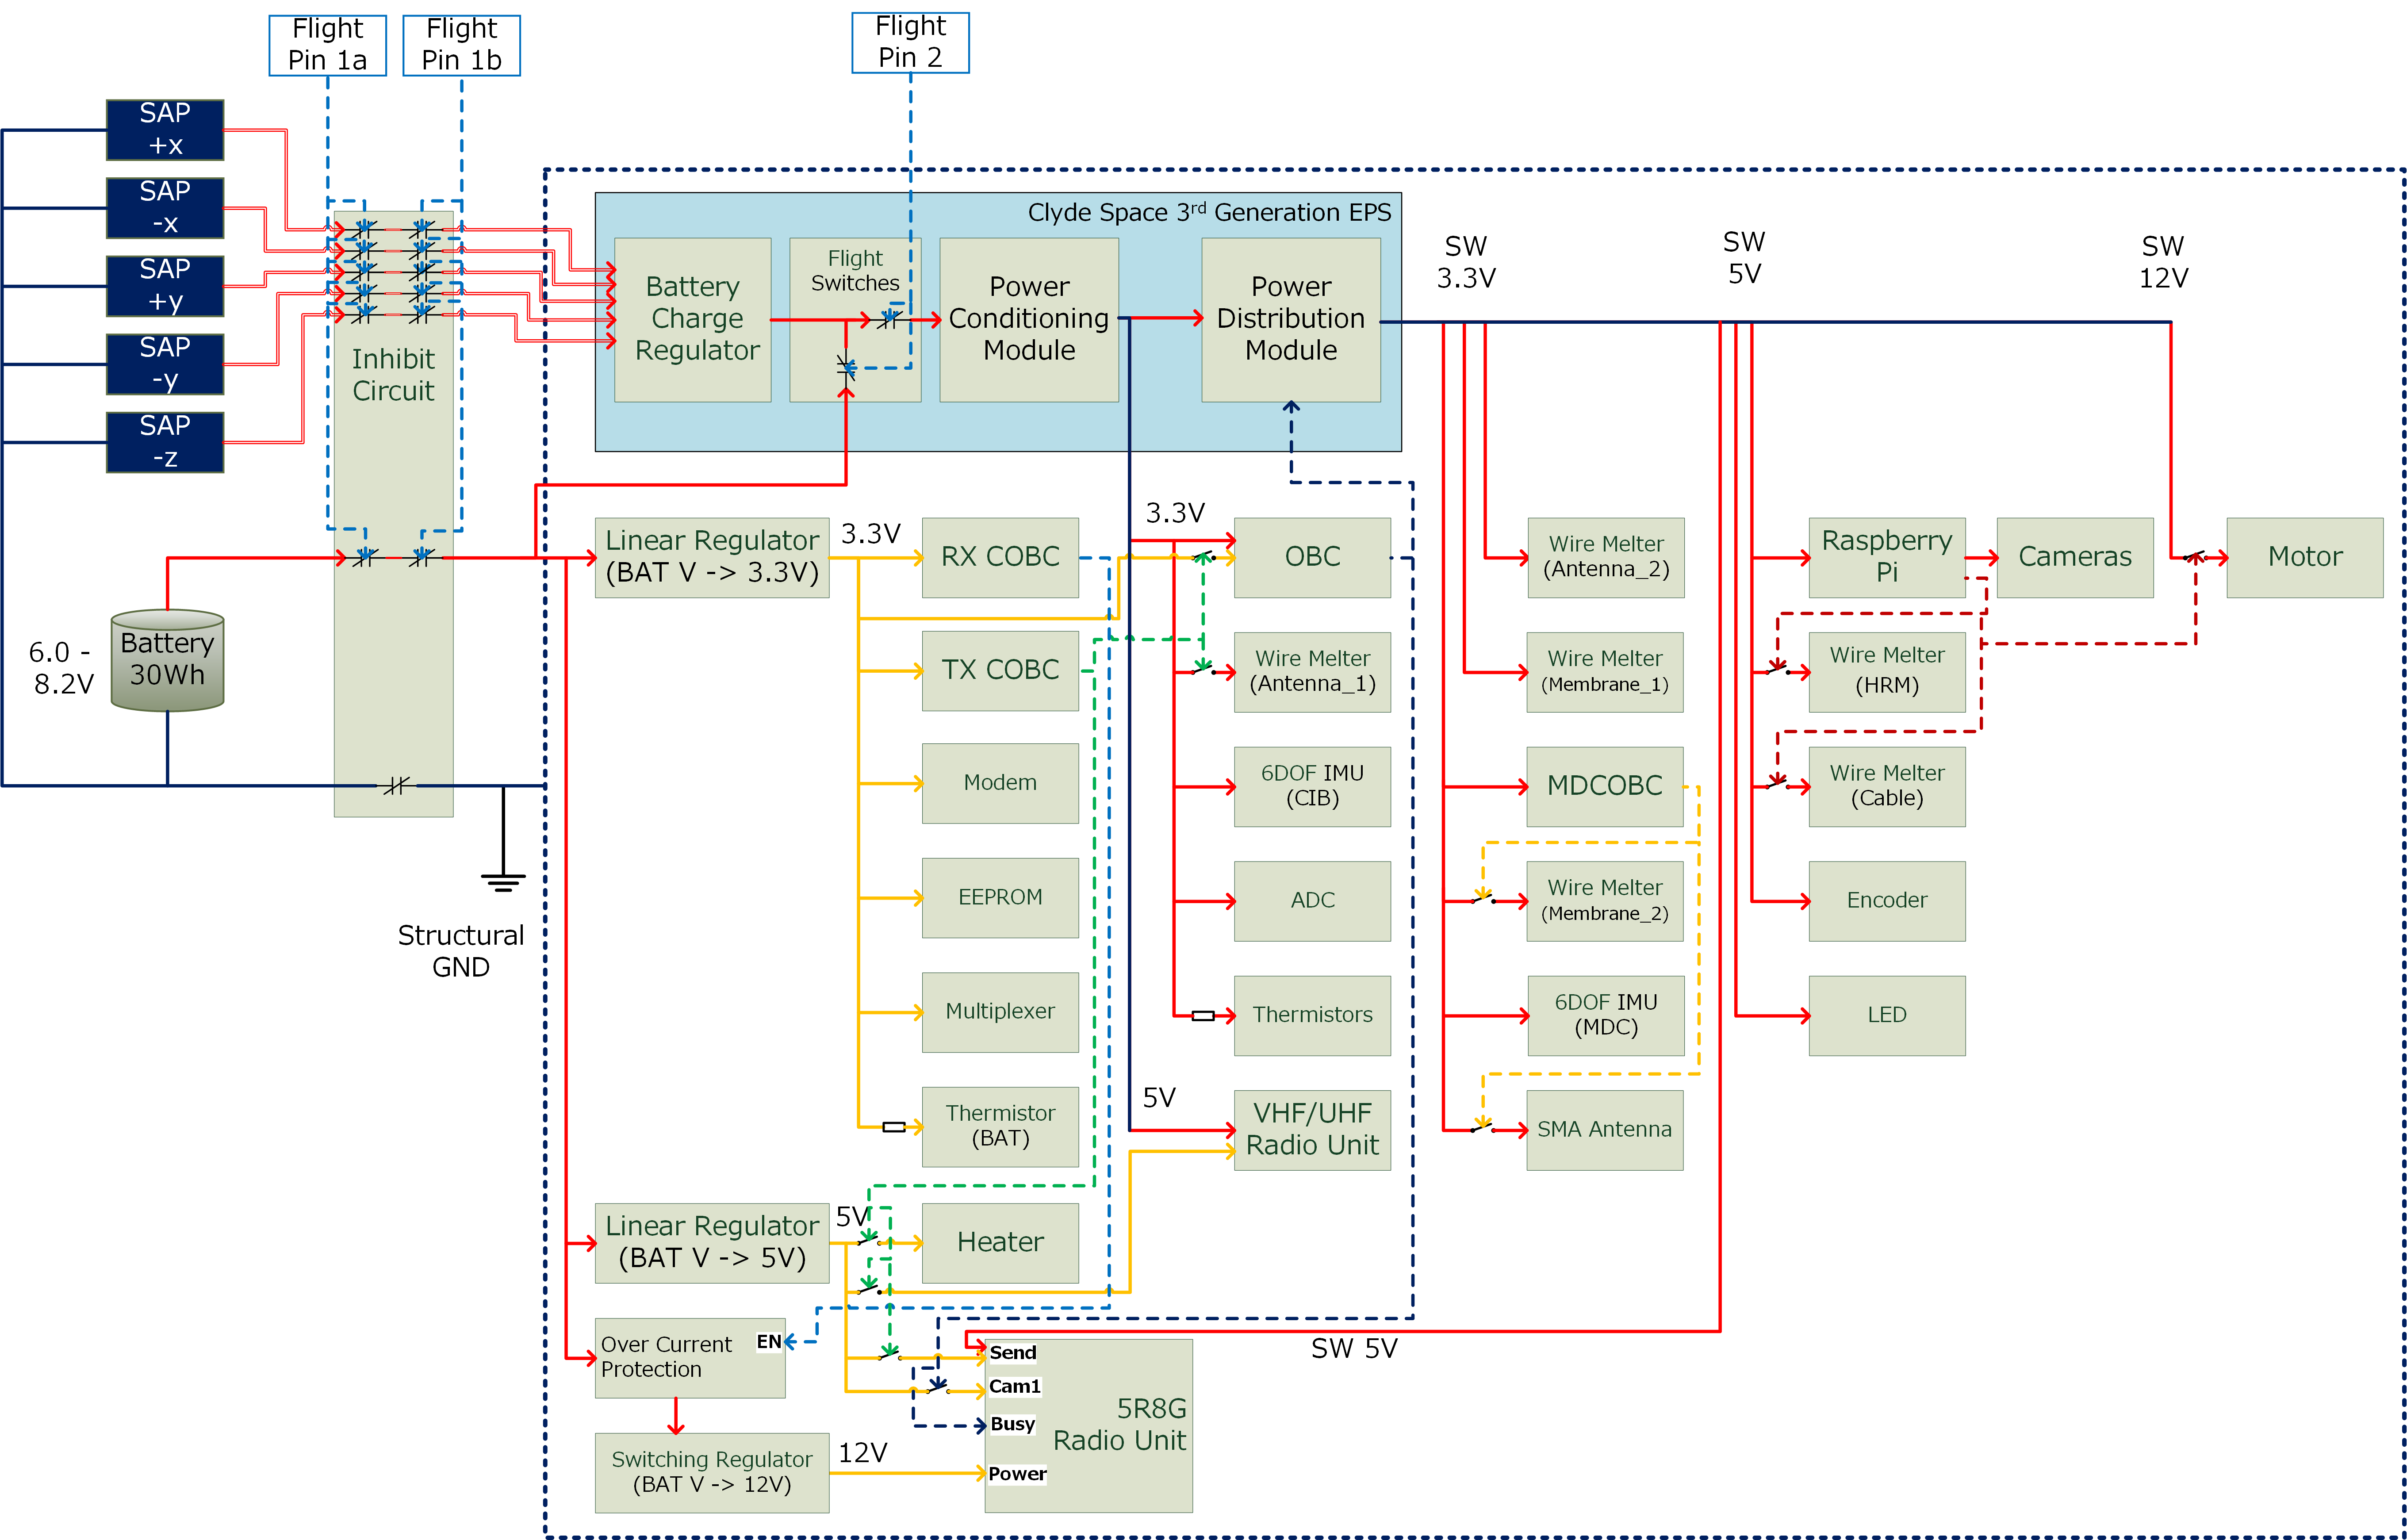
\includegraphics[width=0.8\linewidth]{./03/fig/Power_diagram.png}
		\caption{Example of a figure caption.}
		\label{3_1_power_diagram}
	\end{figure}
\end{landscape}    
\subsection{SAP}

\subsubsection{SAP試験}
\subsection{バッテリ}
バッテリは公称電圧7.6V,放電容量3900mAhのClyde Space社の30Wh Standalone CubeSat Batteryを購入した(図\ref{fig3_1_bat}).バッテリの電気・構造的特性を表\ref{table3_1_bat_spec}に,絶対最大定格を表\ref{table3_1_bat_max}に示す.このバッテリパックは2直3並列のリチウムポリマー電池であり,UN勧告適合品,NASA標準EP-Wi-032適合品である.

\begin{figure}[htbp]
	\begin{center}
		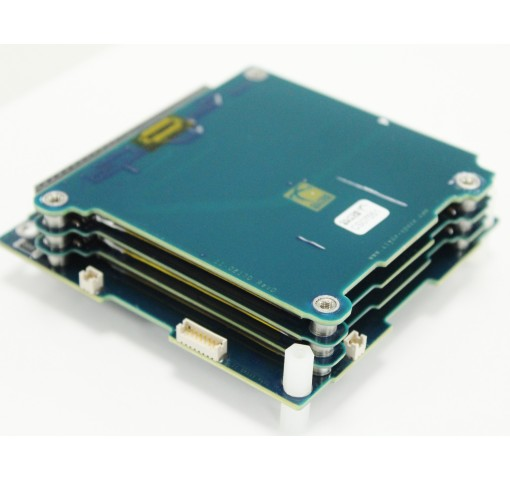
\includegraphics[width=0.5\linewidth]{./03/fig/battery.jpg}
		\caption{30Wh Standalone CubeSat Battery (c)Clyde Space}
		\label{fig3_1_bat}
	\end{center}
\end{figure}

\begin{table}[htbp]
	\begin{center}
		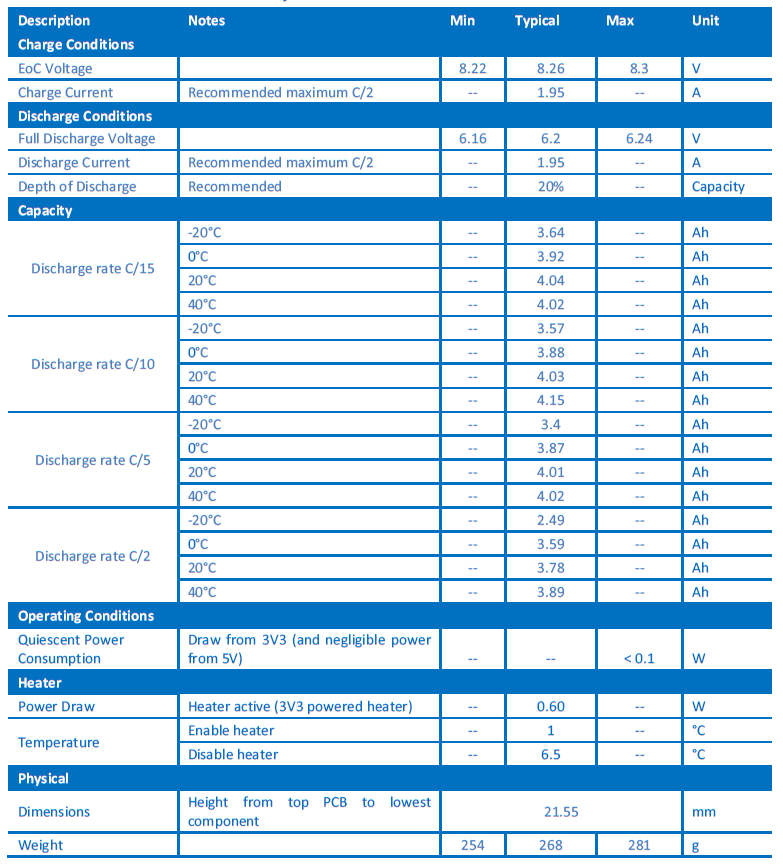
\includegraphics[width=0.9\linewidth]{./03/fig/battery_spec.png}
		\caption{Electrical and Physical Characteristics of Battery \cite{bat_um}}
		\label{table3_1_bat_spec}
	\end{center}
\end{table}


\begin{table}
	\caption{Maximum Ratings of Battery \cite{bat_um}}
	\label{table3_1_bat_max}
	\centering
	\begin{tabular}{ccccc}
		\hline \hline
		\multicolumn{5}{c}{Max Ratings Over Operating Temperature Range (Unless Otherwise Stated)}\\
		&&BCR  & Value  &  Unit  \\
		\hline
		\multirow{3}{*}{Charge Limits}&Voltage&max&8.4&V\\
		&Current&max&6&A\\
		&Current Rate& max &1.53C &Fraction of Capacity\\
		\hline
		\multirow{3}{*}{Discharge Limits}&Voltage&max&6.2&V\\
		&Current&max&6&A\\
		&Current Rate& max &1.53C &Fraction of Capacity\\
		\hline
		\multicolumn{2}{c}{Operating Temperature}&\multicolumn{2}{c}{ -10 to 50} & ${}^\circ$C\\
		\multicolumn{2}{c}{\multirow{3}{*}{Storage Temperature}}&\multicolumn{2}{c}{1 Year: -20 to +20}&\multirow{3}{*}{${}^\circ$C}\\
		&&\multicolumn{2}{c}{3 Months: -20 to +45}&\\
		&&\multicolumn{2}{c}{1 Month: -20 to +60}&\\
		\multicolumn{2}{c}{Vacuum}&\multicolumn{2}{c}{10-5}&torr\\
		\multicolumn{2}{c}{Vibration}&\multicolumn{2}{c}{To [RD-3]}\\
		\hline
	\end{tabular}
\end{table}
	
本バッテリにはセルレベルの過電流,過充電,過放電保護回路(図\ref{fig3-1bat_cpr}),および1並列ごとの過電流保護回路が組み込まれている(図\ref{fig3-1bat_pr}).これらの保護機能については,Clyde Space社から試験報告書を入手し,さらに本衛星開発チームで環境試験(振動,衝撃)前後での充放電特性を測定した(\ref{subsec:bat_test}参照).

また$0^\circ$C以下で自動で動作するヒータが組み込まれており,さらに温度関係なく制御可能な自作ヒータを貼り付けた(図\ref{fig3-1heater}).

FMおよびEMにおいてはバッテリの$\mathrm{I^{2}C}$ラインの故障が生じたために,組み込まれていたテレメトリ取得機能が使用不可能となった.バッテリの電圧,温度等の情報は別系統で取得可能にしていた.
\begin{figure}[htbp]
	\begin{minipage}{0.5\hsize}
		\begin{center}
			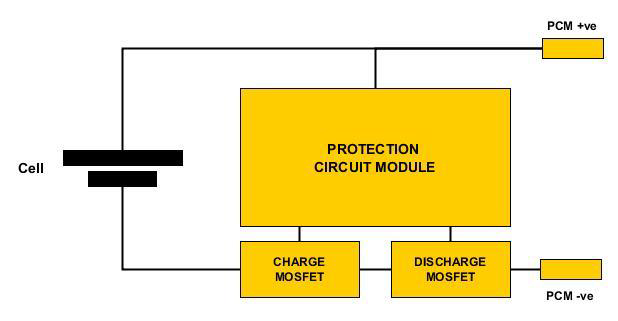
\includegraphics[height=0.5\linewidth]{./03/fig/cell_protection.png}
			\caption{Cell Level Protection Circuit Schematic \cite{bat_um}}
			\label{fig3-1bat_cpr}
		\end{center}
	\end{minipage}
	\begin{minipage}{0.5\hsize}
		\begin{center}
			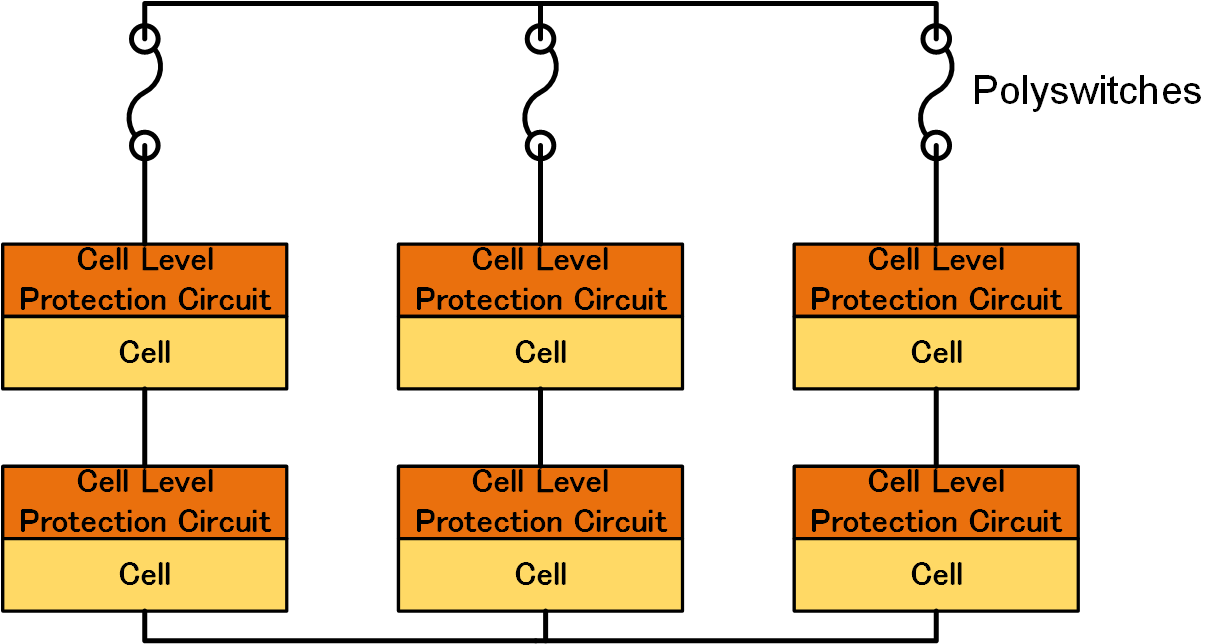
\includegraphics[height=0.5\linewidth]{./03/fig/bat_pr.png}
			\caption{Battery Protection Architecture}
			\label{fig3-1bat_pr}
		\end{center}
	\end{minipage}
\end{figure}

\begin{figure}[htbp]
	\begin{center}
		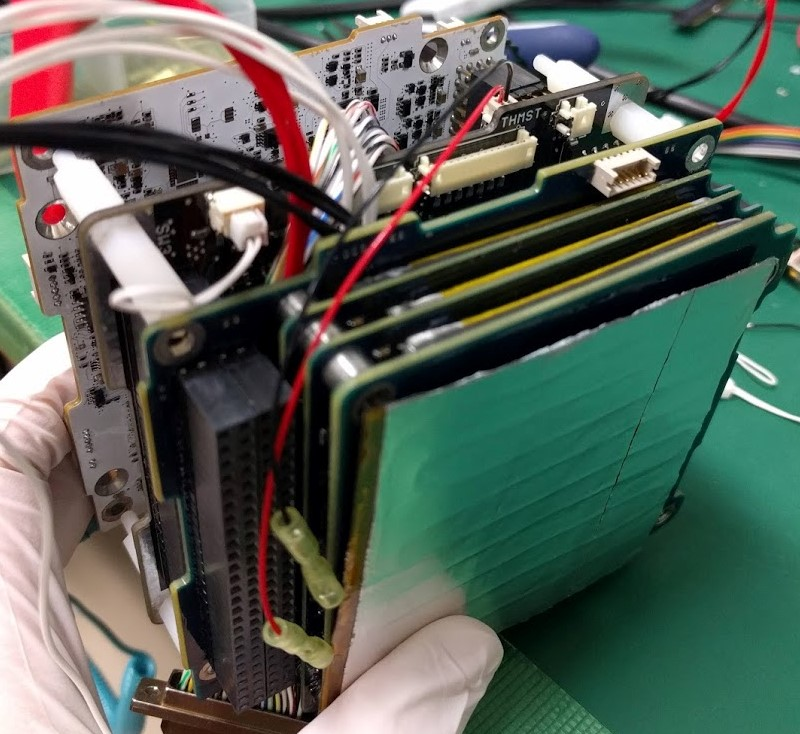
\includegraphics[width=0.5\linewidth]{./03/fig/heater.jpg}
		\caption{Image of Heater on Battery}
		\label{fig3-1heater}
	\end{center}
\end{figure}

\subsection{CIB電源系}

\begin{figure}[htbp]
	\begin{minipage}{0.5\hsize}
		\begin{center}
			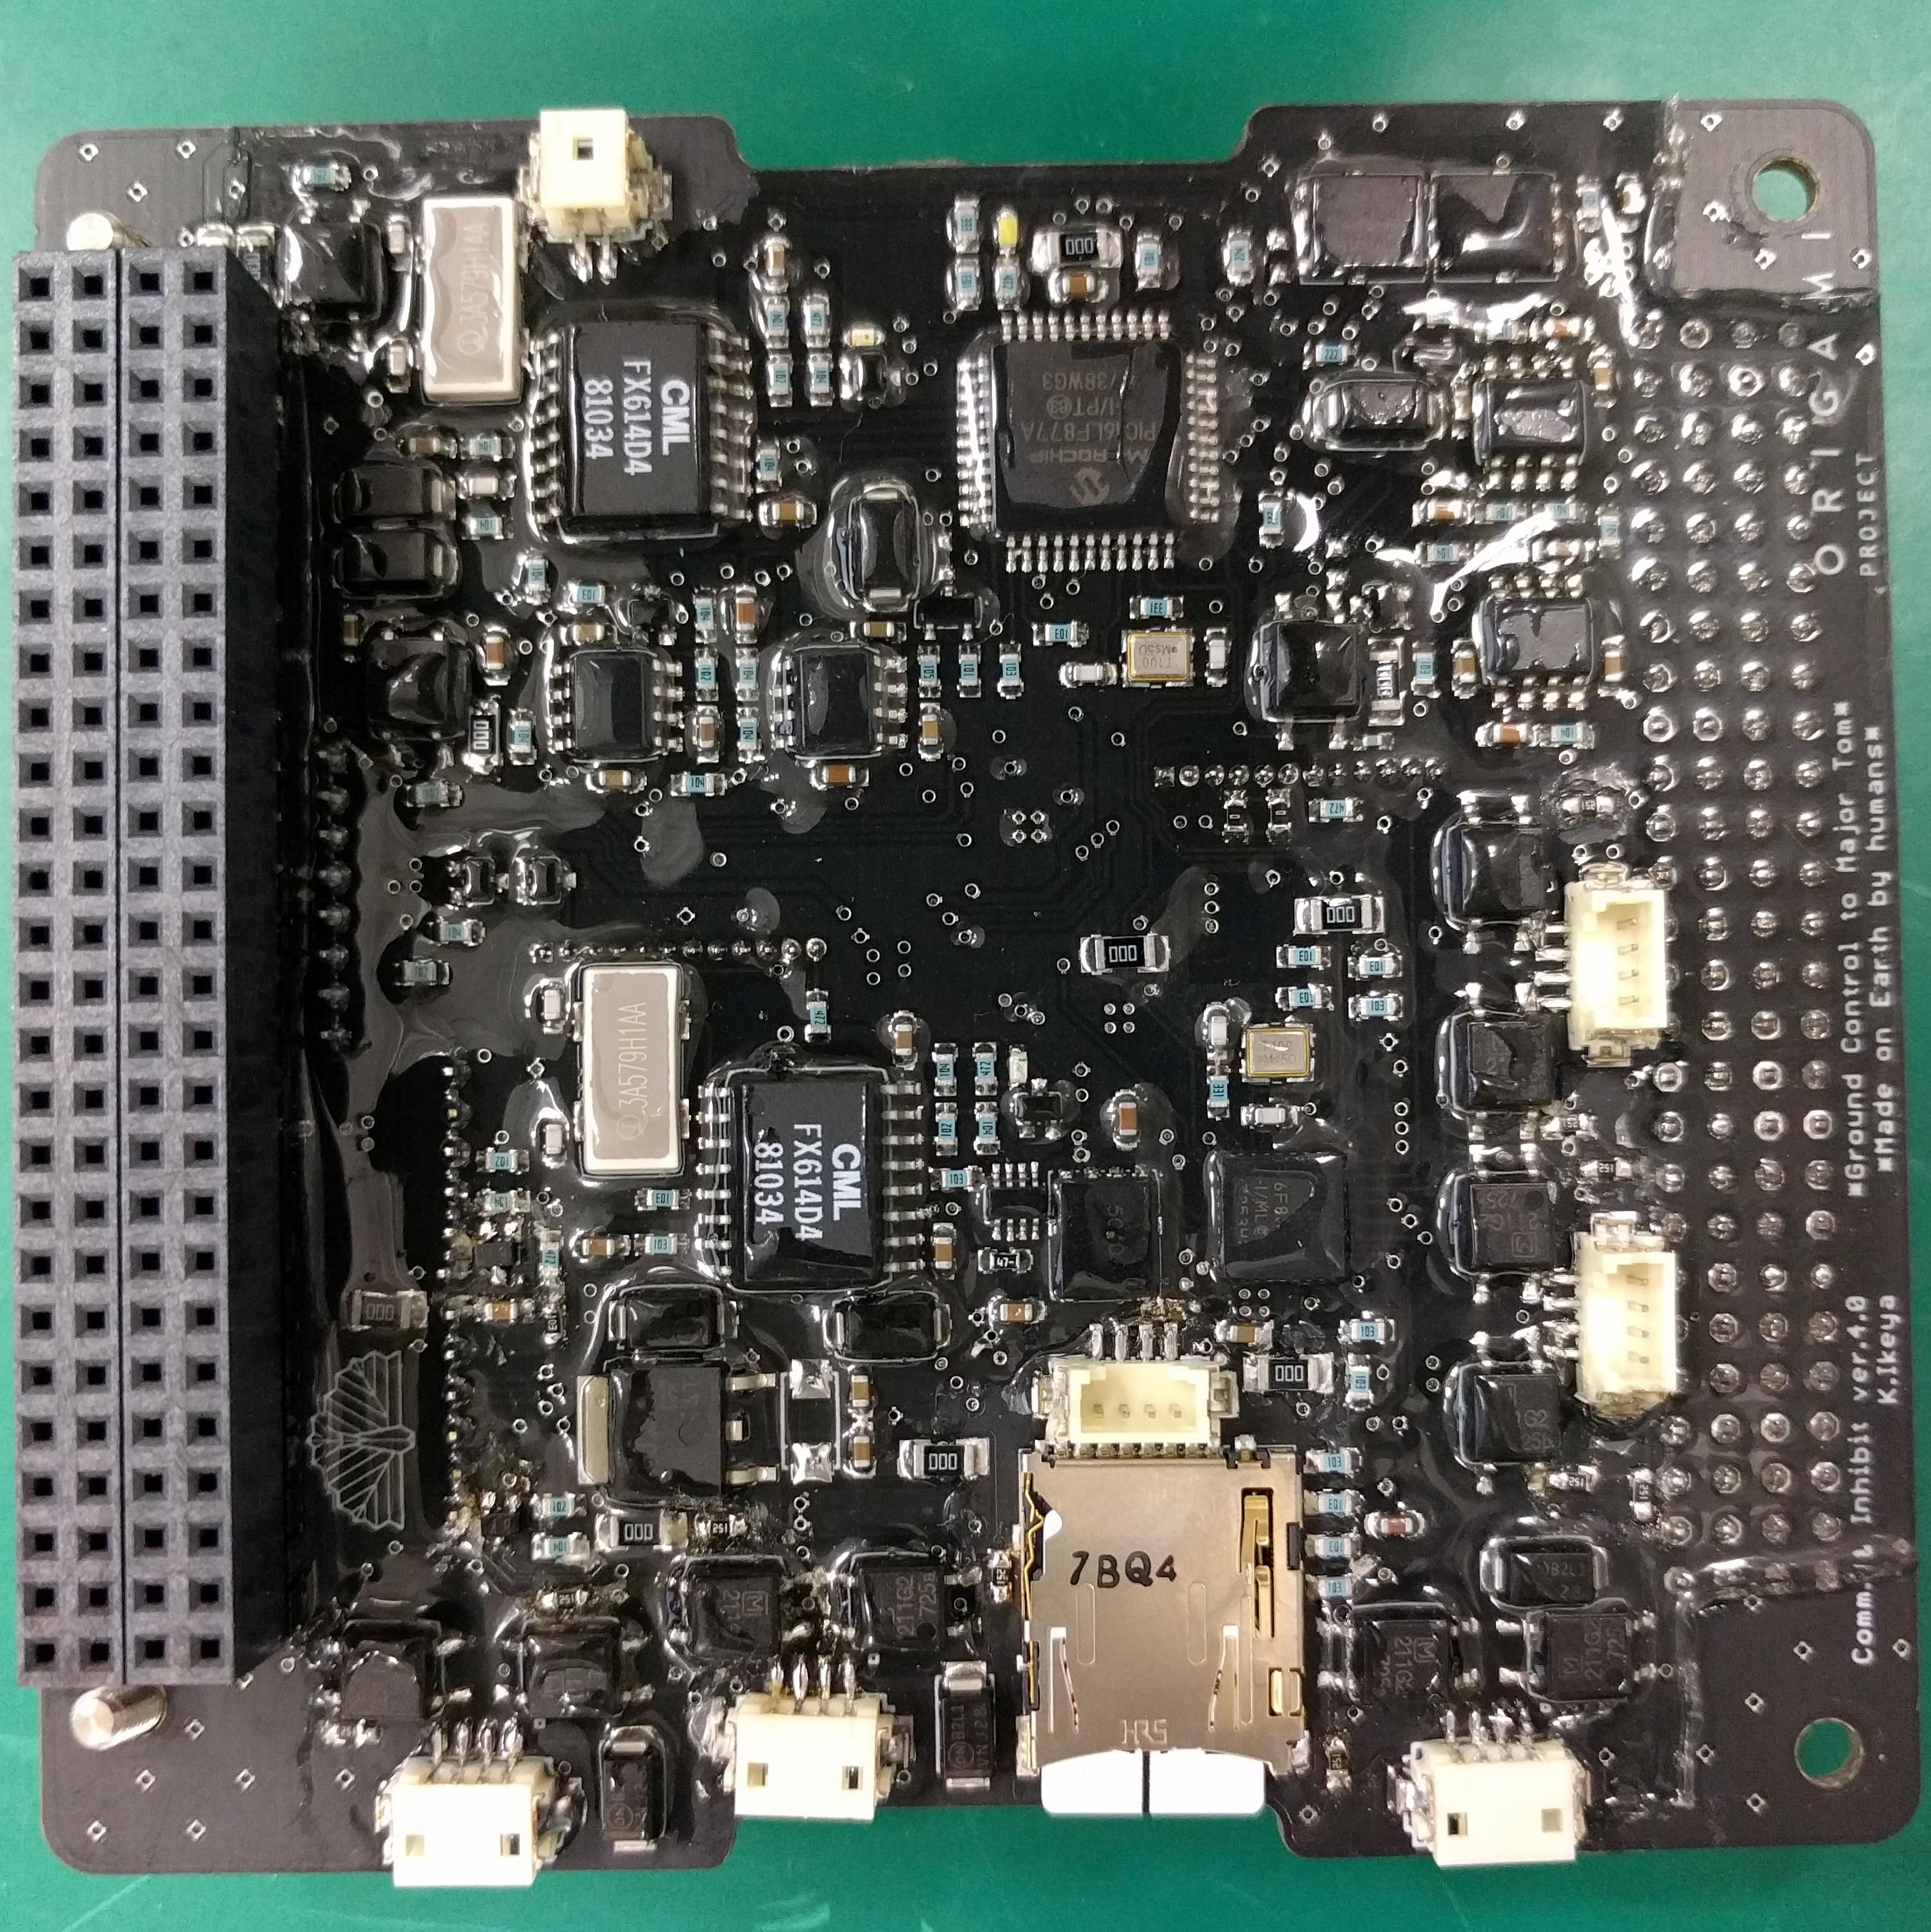
\includegraphics[width=0.7
			\linewidth]{./03/fig/CIB_1.jpg}
		\end{center}
	\end{minipage}
	\begin{minipage}{0.5\hsize}
		\begin{center}
			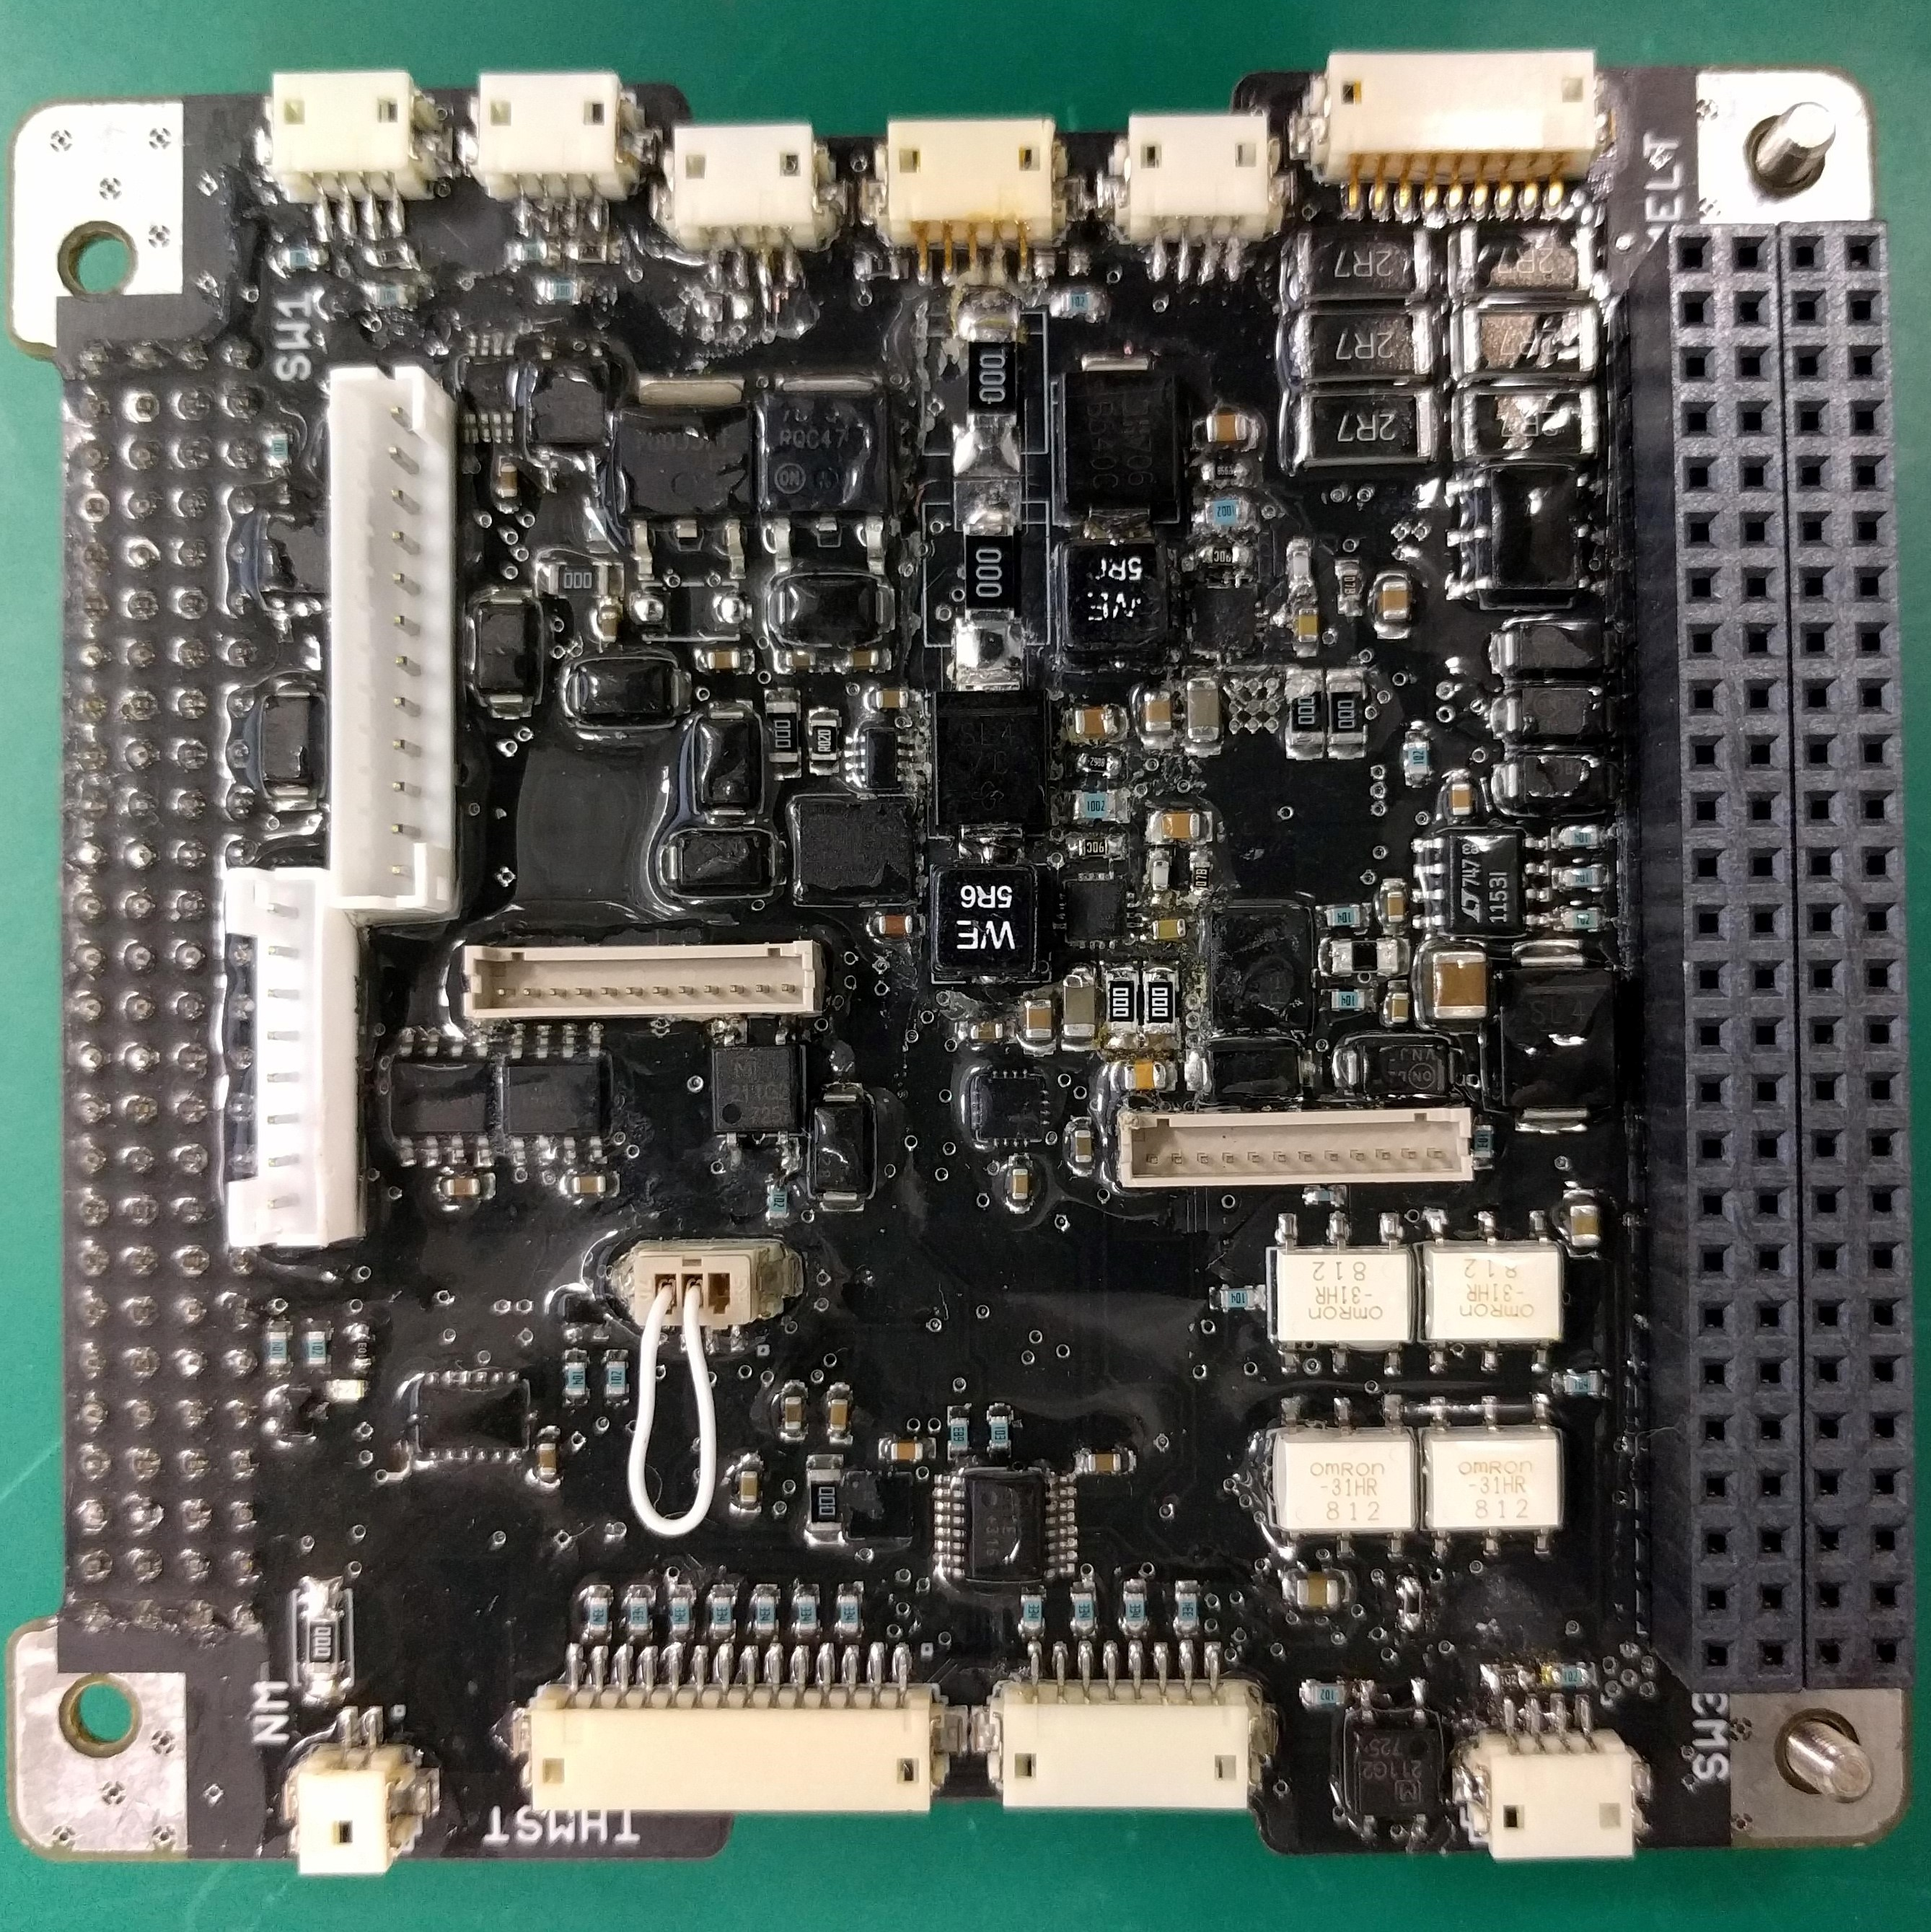
\includegraphics[width=0.7\linewidth]{./03/fig/CIB_2.jpg}
		\end{center}
	\end{minipage}\\		
	\begin{center}
		\caption{CIB}
	\end{center}
\label{CIB}
\end{figure}

\subsubsection{インヒビット回路}
イプシロンロケット
ACX-11007「小型副衛星の安全設計手引き制定初版」を参考に
要求により

以下のハザードを設けられた
これらのハザードに対応するために
3インヒビット回路を設けた.

購入品ではこれらの要求を満たせなかったため新たに

Battery-EPS間に新たに

ただし現在は3インヒビット要求を満たすバッテリがClyde Space社から新たに発売されている

\begin{figure}[htbp]
	\begin{center}
		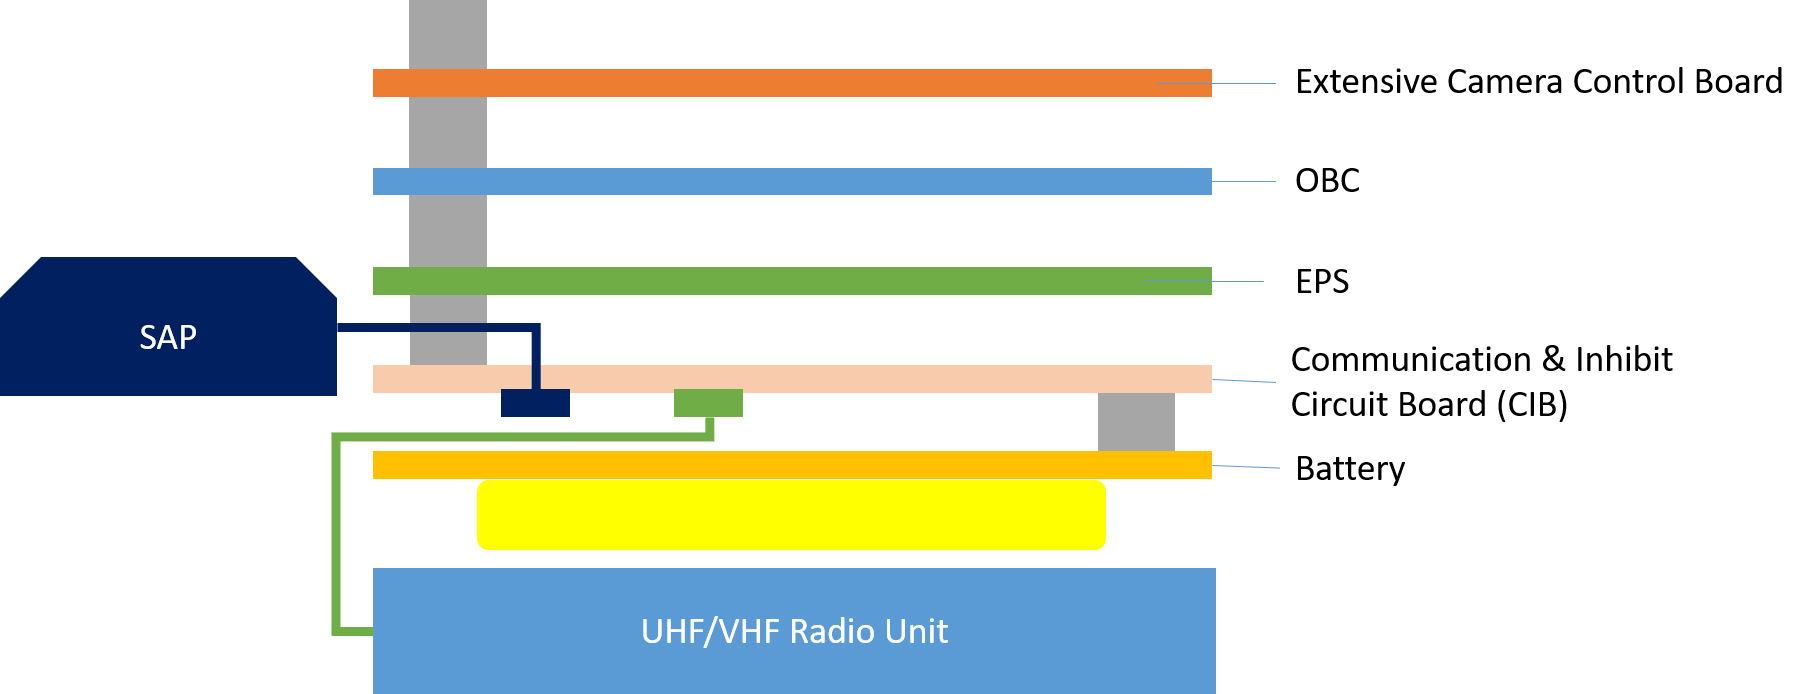
\includegraphics[width=0.7\linewidth]{./03/fig/cib_position.png}
		\caption{Cell level protection circuit schematic 転載}
		\label{fig3_1_cibposi}
	\end{center}
\end{figure}
インヒビット回路の回路図は

のようになっている

SAP-EPS間の遮断


リターン側のMOSFETをBack to Back
で双方向
実際には片方のみで問題ない
HOT側のPhotoMOSは
型番


これらのIC選定の基準として

またP-chanel MOS

回路の簡易化のために
ただしMOS
内部抵抗は概して小さい
これらのIC動作の不具合は致命的であるため
実際には並列に接続した

\begin{figure}[htbp]
	\begin{center}
		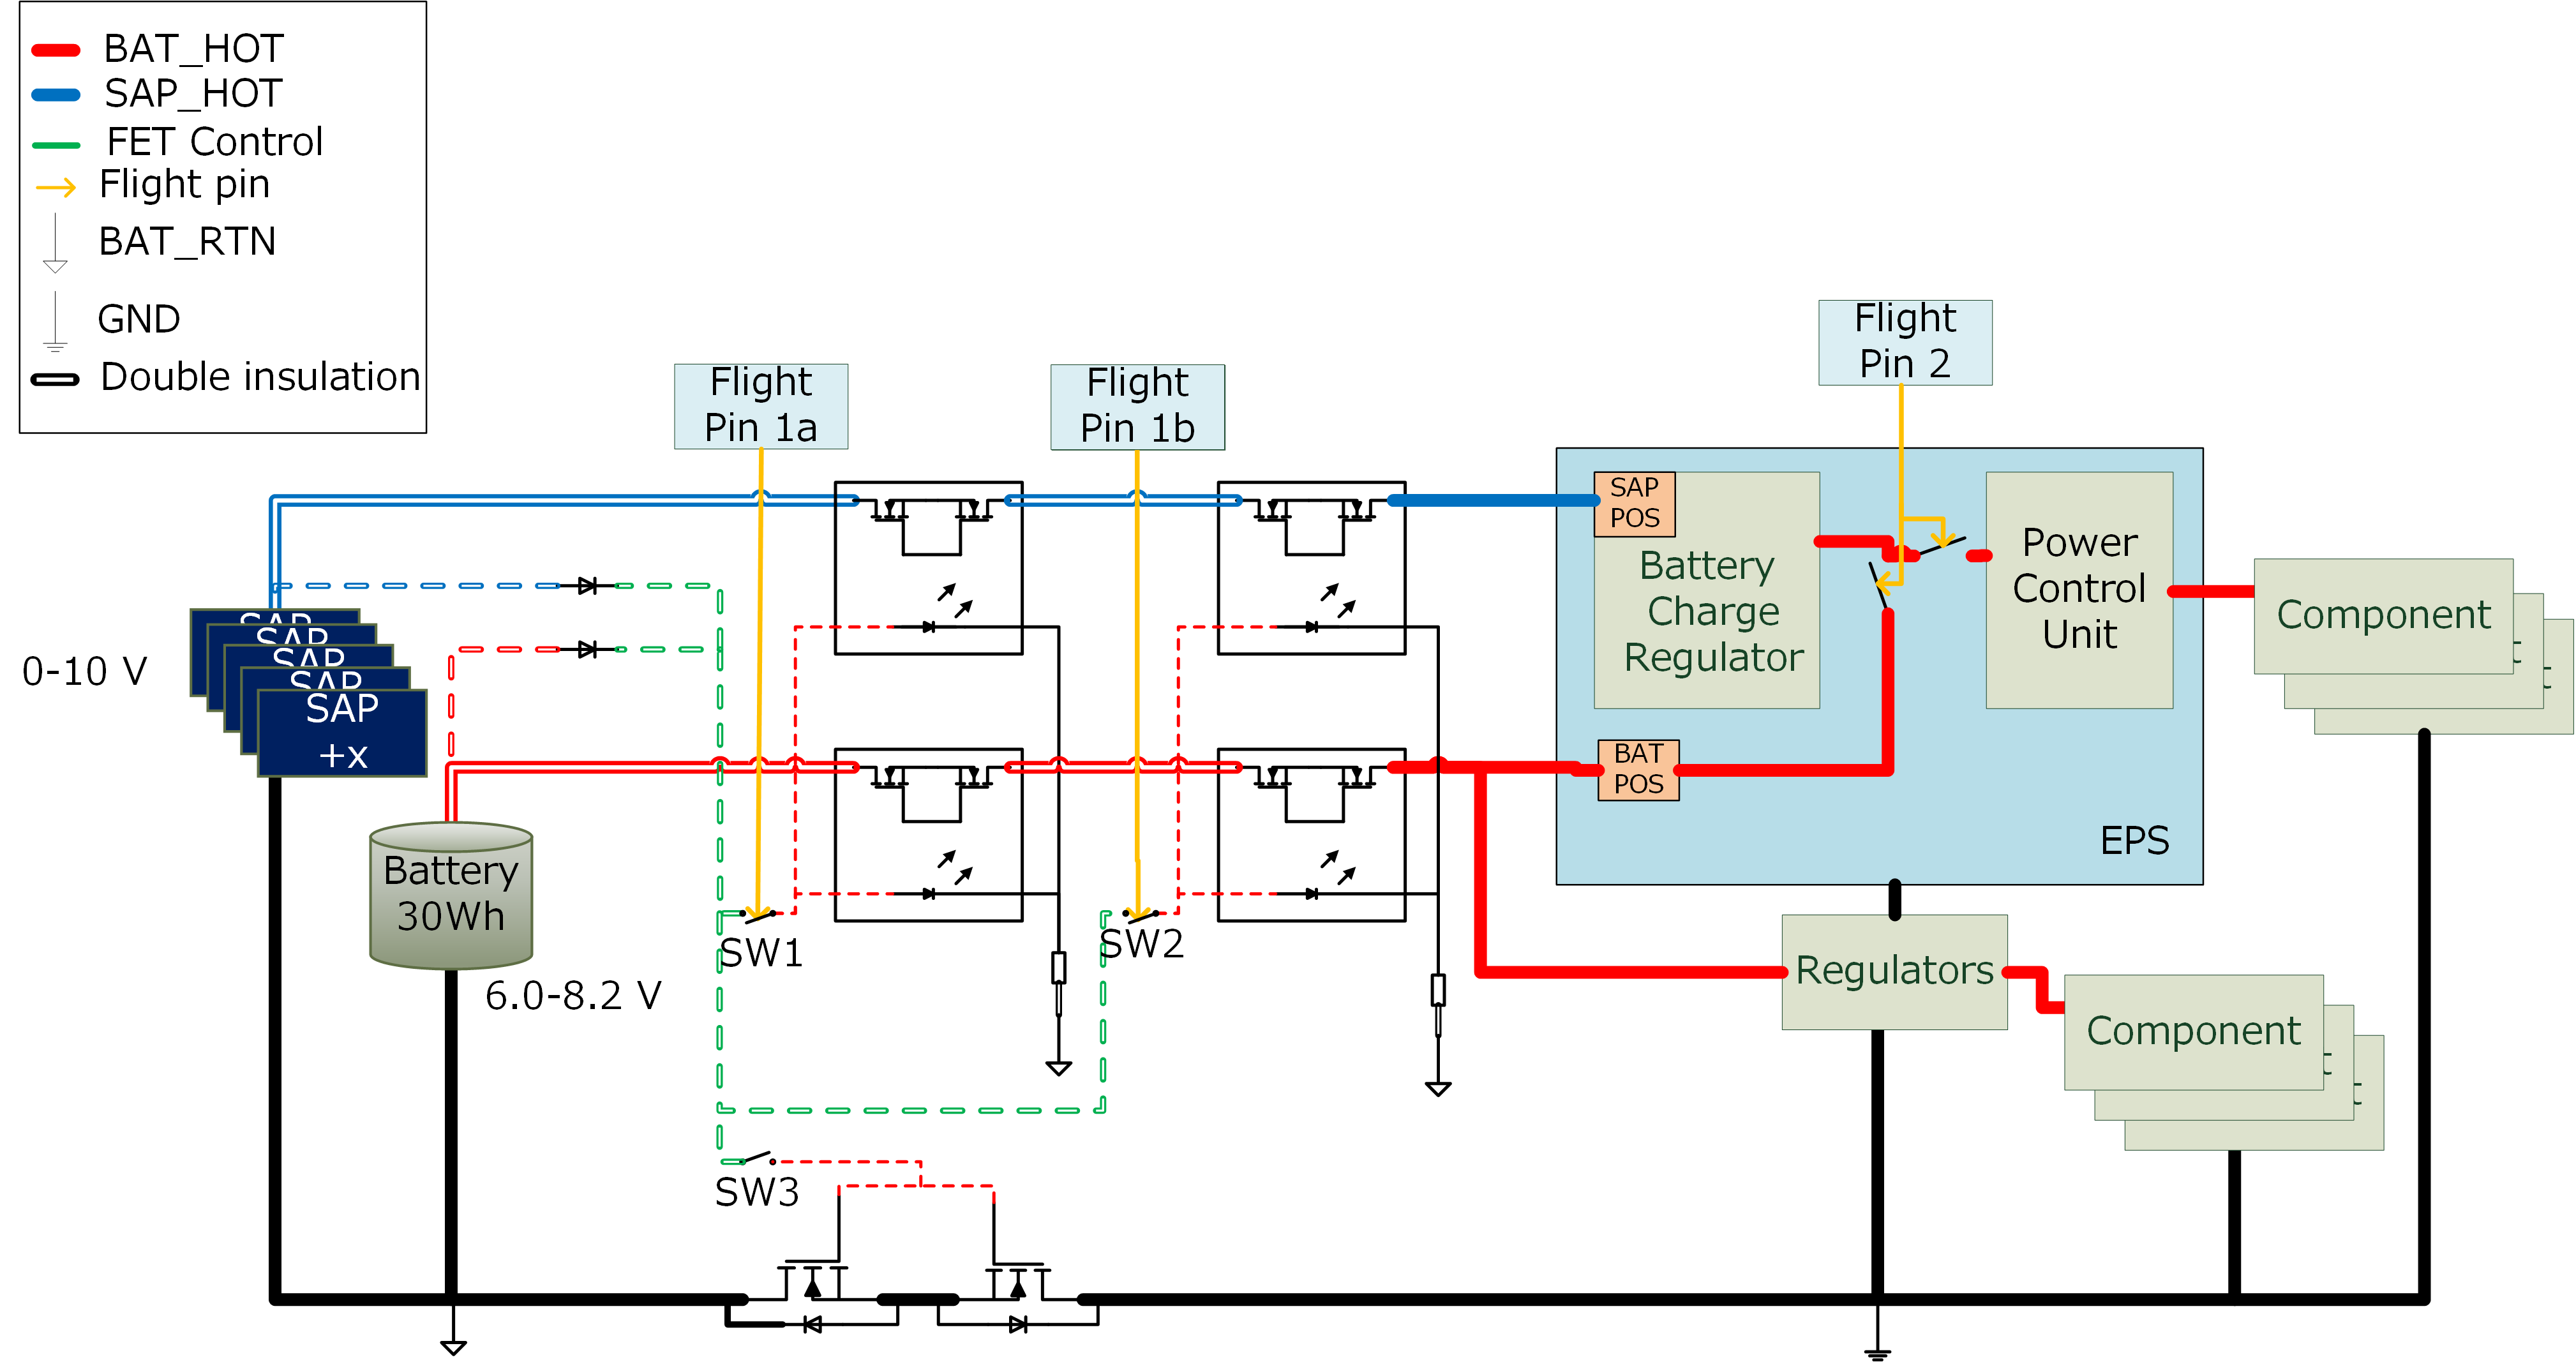
\includegraphics[width=0.9\linewidth]{./03/fig/inhibit_diagram_2.png}
		\caption{Integrated EPS and Battery Protection Architecture 転載}
		\label{fig3_1_inhibit_d}
	\end{center}
\end{figure}

\subsubsection{フライトピン}
衛星のハンドリング中




\subsubsection{CIB内電源回路}
通信用マイコンであるRXCOBC,TXCOBCはミッション開始から終了までほぼすべての期間で起動している必要がある.EPSから供給されるコンポーネントの一括on/offを可能にするためにこれらの電源系はEPS基板とは別に新たに設け,EPS電源が入っていない状態においても衛星として最低限の役割が機能するように設計した.




そこで新たな電源回路をCIB内に設けた.RXCOBC,TXCOBCの電源である3.3 V系は軌道上での故障が許されない
そこで一般的に効率の良いスイッチングレギュレータ,ではなく信頼性の高い三端子レギュレータを使用した.さらにレギュレータが1つ動作しなかった場合に備えて二つのレギュレータを並列で繋いだ.

参考文献


\begin{figure}[htbp]
	\begin{center}
		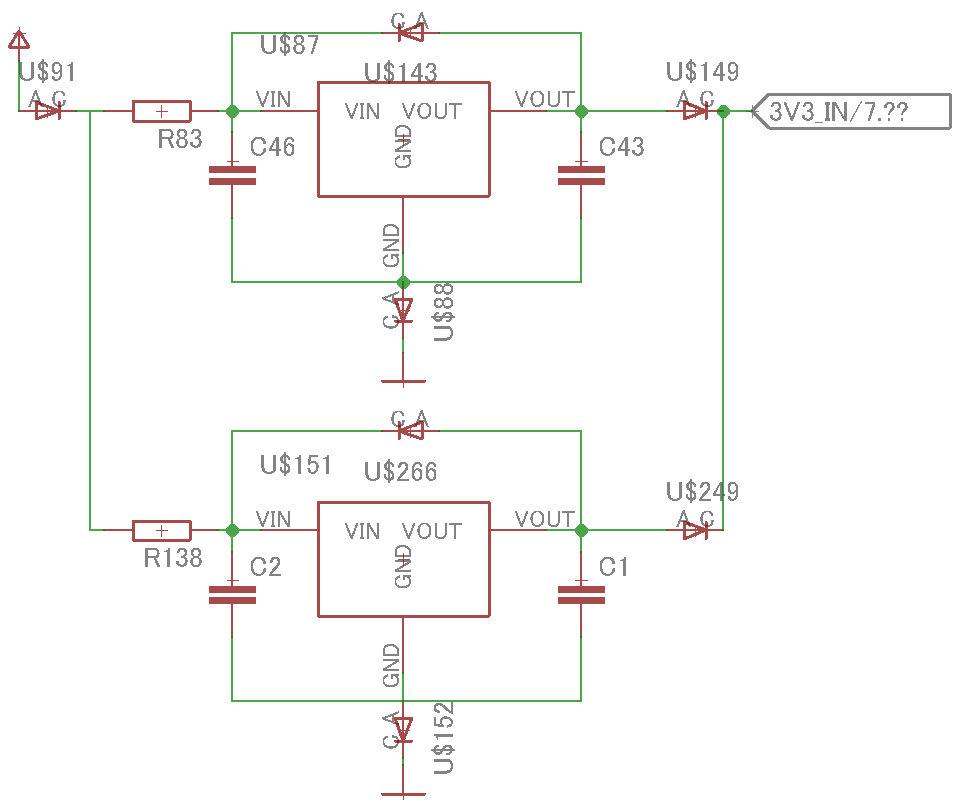
\includegraphics[width=0.6\linewidth]{./03/fig/3V3.png}
		\caption{Integrated EPS and Battery Protection Architecture 転載}
		\label{fig3_1_inhibit_d}
	\end{center}
\end{figure}

およびUHF/VHF無線機


また5.8GHz送信を行う際の突入電流が非常に大きくEPSの
保護機能が働いてしまうために12V系も新たにCIB上に設計した


12V系は
突入電流が
購入EPSの

そこで新たにDC-DCコンバータ

これらは二重に

さらに過電流対策

放射線試験によるICの放射線耐性を




\subsection{放出検知スイッチ・フライトピン}
図\ref{fig3_1_inhibit_d}中のSW1, SW2, SW3は放出検知スイッチであり,放出検知ピンにより開放・短絡が制御される(図\ref{fig3-1pin}).

\begin{figure}[htbp]
	\begin{minipage}{0.32\hsize}
		\centering
		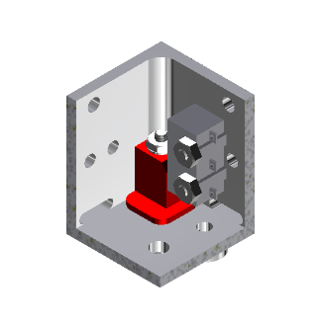
\includegraphics[height=0.7\linewidth]{./03/fig/pin_a.png}
		\subcaption{Oblique View}
	\end{minipage}
	\begin{minipage}{0.32\hsize}
		\centering
		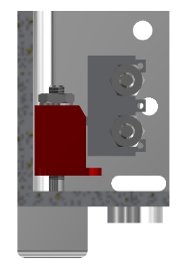
\includegraphics[height=0.7\linewidth]{./03/fig/pin_b.png}
		\subcaption{Pushed State}
	\end{minipage}
	\begin{minipage}{0.32\hsize}
		\centering
		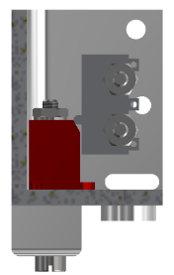
\includegraphics[height=0.7\linewidth]{./03/fig/pin_c.png}
		\subcaption{Released State}
	\end{minipage}
	\caption{Release Detection Pin}
	\label{fig3-1pin}
\end{figure}


放出ポッド搭載までの意図せぬ電源投入を防ぐためにフライトピンを設けた.本衛星には放出検知ピンを機械的にロックするフライトピン(1a,1b,図\ref{fig3-1fpin})と電気的にEPS以降の起動を阻止するフライトピン2がある.

\begin{figure}[htbp]
	\begin{minipage}{\hsize}
		\centering
		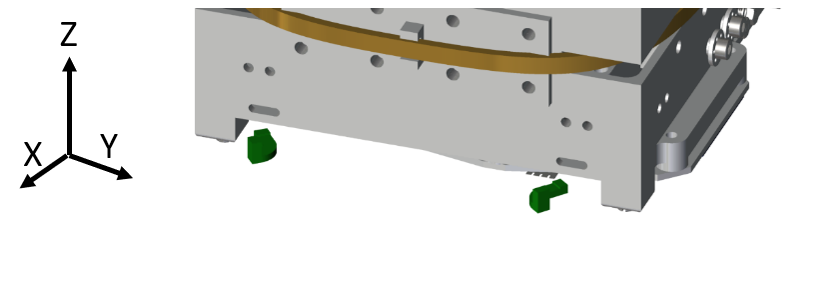
\includegraphics[width=0.5\linewidth]{./03/fig/fpin_a.png}
		\subcaption{Oblique View}
	\end{minipage}\\
	\begin{minipage}{0.5\hsize}
		\centering
		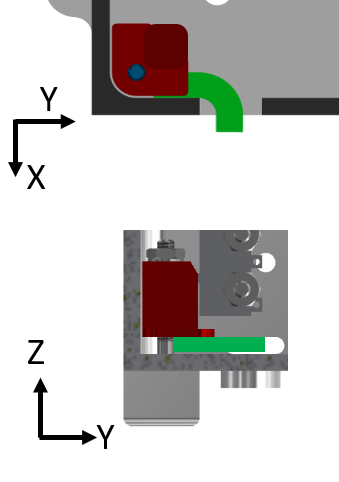
\includegraphics[height=0.7\linewidth]{./03/fig/fpin_b.png}
		\subcaption{Locked State}
	\end{minipage}
	\begin{minipage}{0.5\hsize}
		\centering
		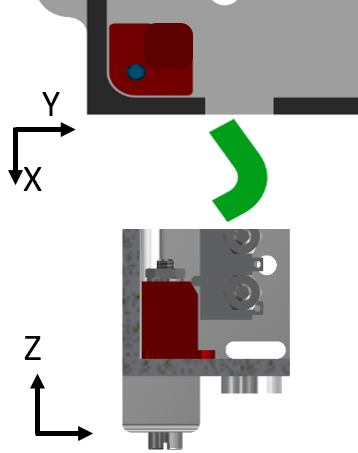
\includegraphics[height=0.7\linewidth]{./03/fig/fpin_c.png}
		\subcaption{Released State}
	\end{minipage}
	\caption{Flight Pin 1}
	\label{fig3-1fpin}
\end{figure}

フライトピン2はEPSの組み込み機能であるSeparation Switch端子とRBF(Remove Before Flight) Switch端子をGNDに導通させることでEPSの起動を防ぐ.


\subsection{CIB内電源回路}



通信用マイコンであるRXCOBC,TXCOBCはミッション開始から終了まで非常時を除きすべての期間で起動している必要がある.EPSから電源供給されるコンポーネントの一括ON/OFFを可能にするためにこれらの電源系はEPS基板とは別に新たに設け,EPS電源が入っていない状態においても衛星として最低限の役割が機能するように設計した.RXCOBC,TXCOBCの電源であるCIB内の3.3 V系には一般的に効率の良いスイッチングレギュレータではなく信頼性の高いリニアレギュレータを使用した.さらにレギュレータが1つ動作しなかった場合に備えて二つのレギュレータを並列で繋いだ(図\ref{fig3_1_3V3}).一般にリニアレギュレータの並列はORダイオードを用いて行われる\cite{reg_um}.

\begin{figure}[htbp]
	\begin{center}
		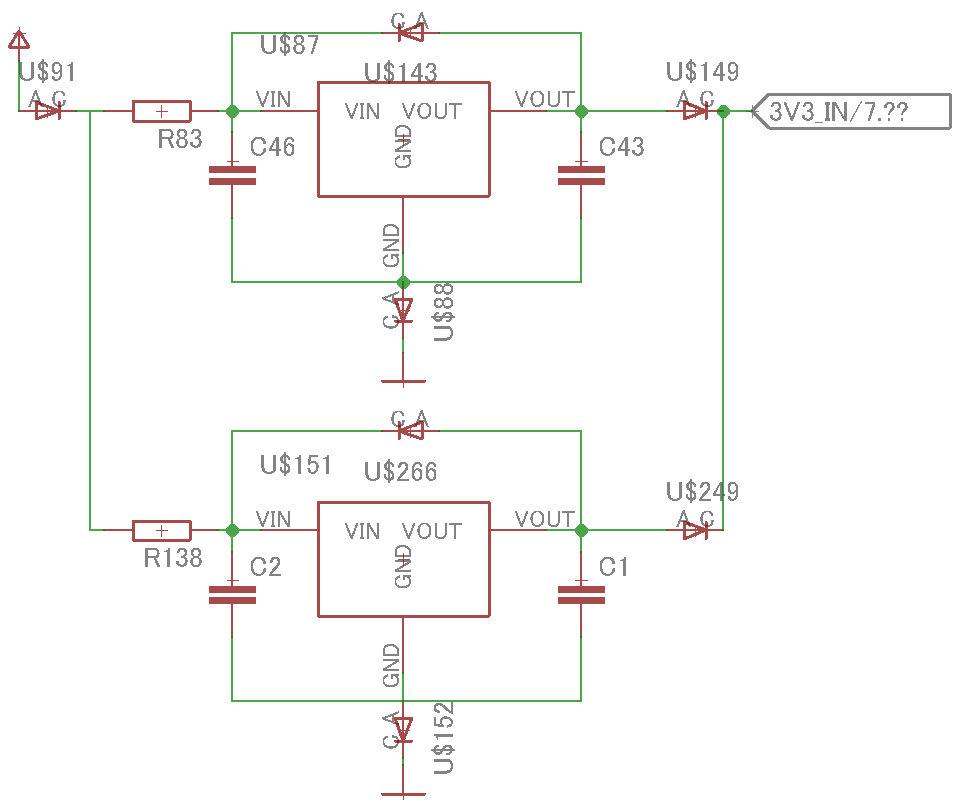
\includegraphics[width=0.6\linewidth]{./03/fig/3V3.png}
		\caption{Paralleling Linear Regulators Schematic}
		\label{fig3_1_3V3}
	\end{center}
\end{figure}

UHF/VHF無線機はEPSからの供給をメインとし,EPS非起動時にも通信が行えるように5VをCIB内でリニアレギュレータを用いて生成できるようにした.

さらに5.8GHz送信を行う際の突入電流によりEPSの過電流保護機能が働き,他の機器への影響がでてしまうため昇圧スイッチング・レギュレータを用いて12V系も新たにCIB上に設計した.さらにレギュレータの故障による過電流防止のために,
ICを設けた.また放射線試験によるICの放射線耐性を入念に確認した.


\subsection{EPS}
EPSはClyde Space社の3rd Generation 3U EPSを購入した.
EPSの電気・構造的特性を表\ref{table3_1_eps_spec}に,絶対最大定格を表\ref{table3_1_eps_max}に示す.
\begin{figure}[htbp]
	\begin{center}
		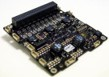
\includegraphics[width=0.5\linewidth]{./03/fig/eps.jpg}
		\caption{EPS}
		\label{eps}
	\end{center}
\end{figure}


\begin{table}[htbp]
	\centering
	\caption{Electrical and Physical Characteristics of EPS \cite{eps_um}}
	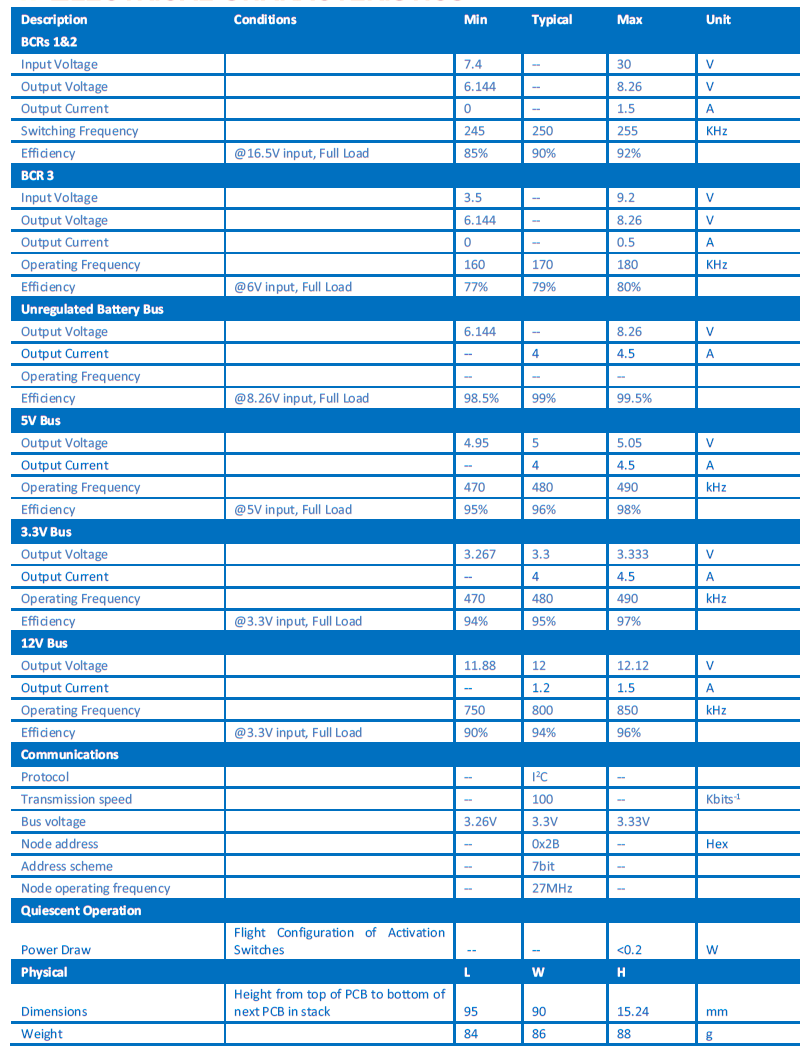
\includegraphics[width=0.9\linewidth]{./03/fig/eps_spec.png}
	\label{table3_1_eps_spec}
\end{table}

\begin{table}[htbp]
	\centering
	\caption{Maximum Ratings of EPS \cite{eps_um}}
	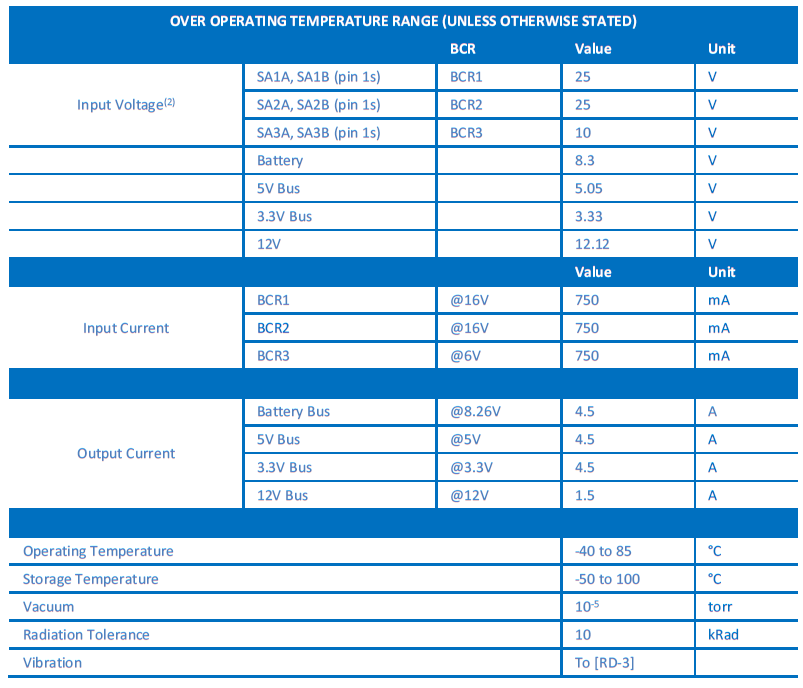
\includegraphics[width=0.9\linewidth]{./03/fig/eps_max.png}
	\label{table3_1_eps_max}
\end{table}


EPSユーザーマニュアル記載のEPSおよびSAP,Batteryを含めた機能図を図\ref{fig3-1_eps_bd}に示す.なお本衛星ではBattery-EPS間,SAP-EPS間にインヒビット回路が組み込まれているため実際のコンフィグレーションとは異なる.EPSの各スイッチのON/OFFはOBCからの$\mathrm{I^{2}C}$によって制御された.

\begin{landscape}
\begin{figure}[H]
	\centering
	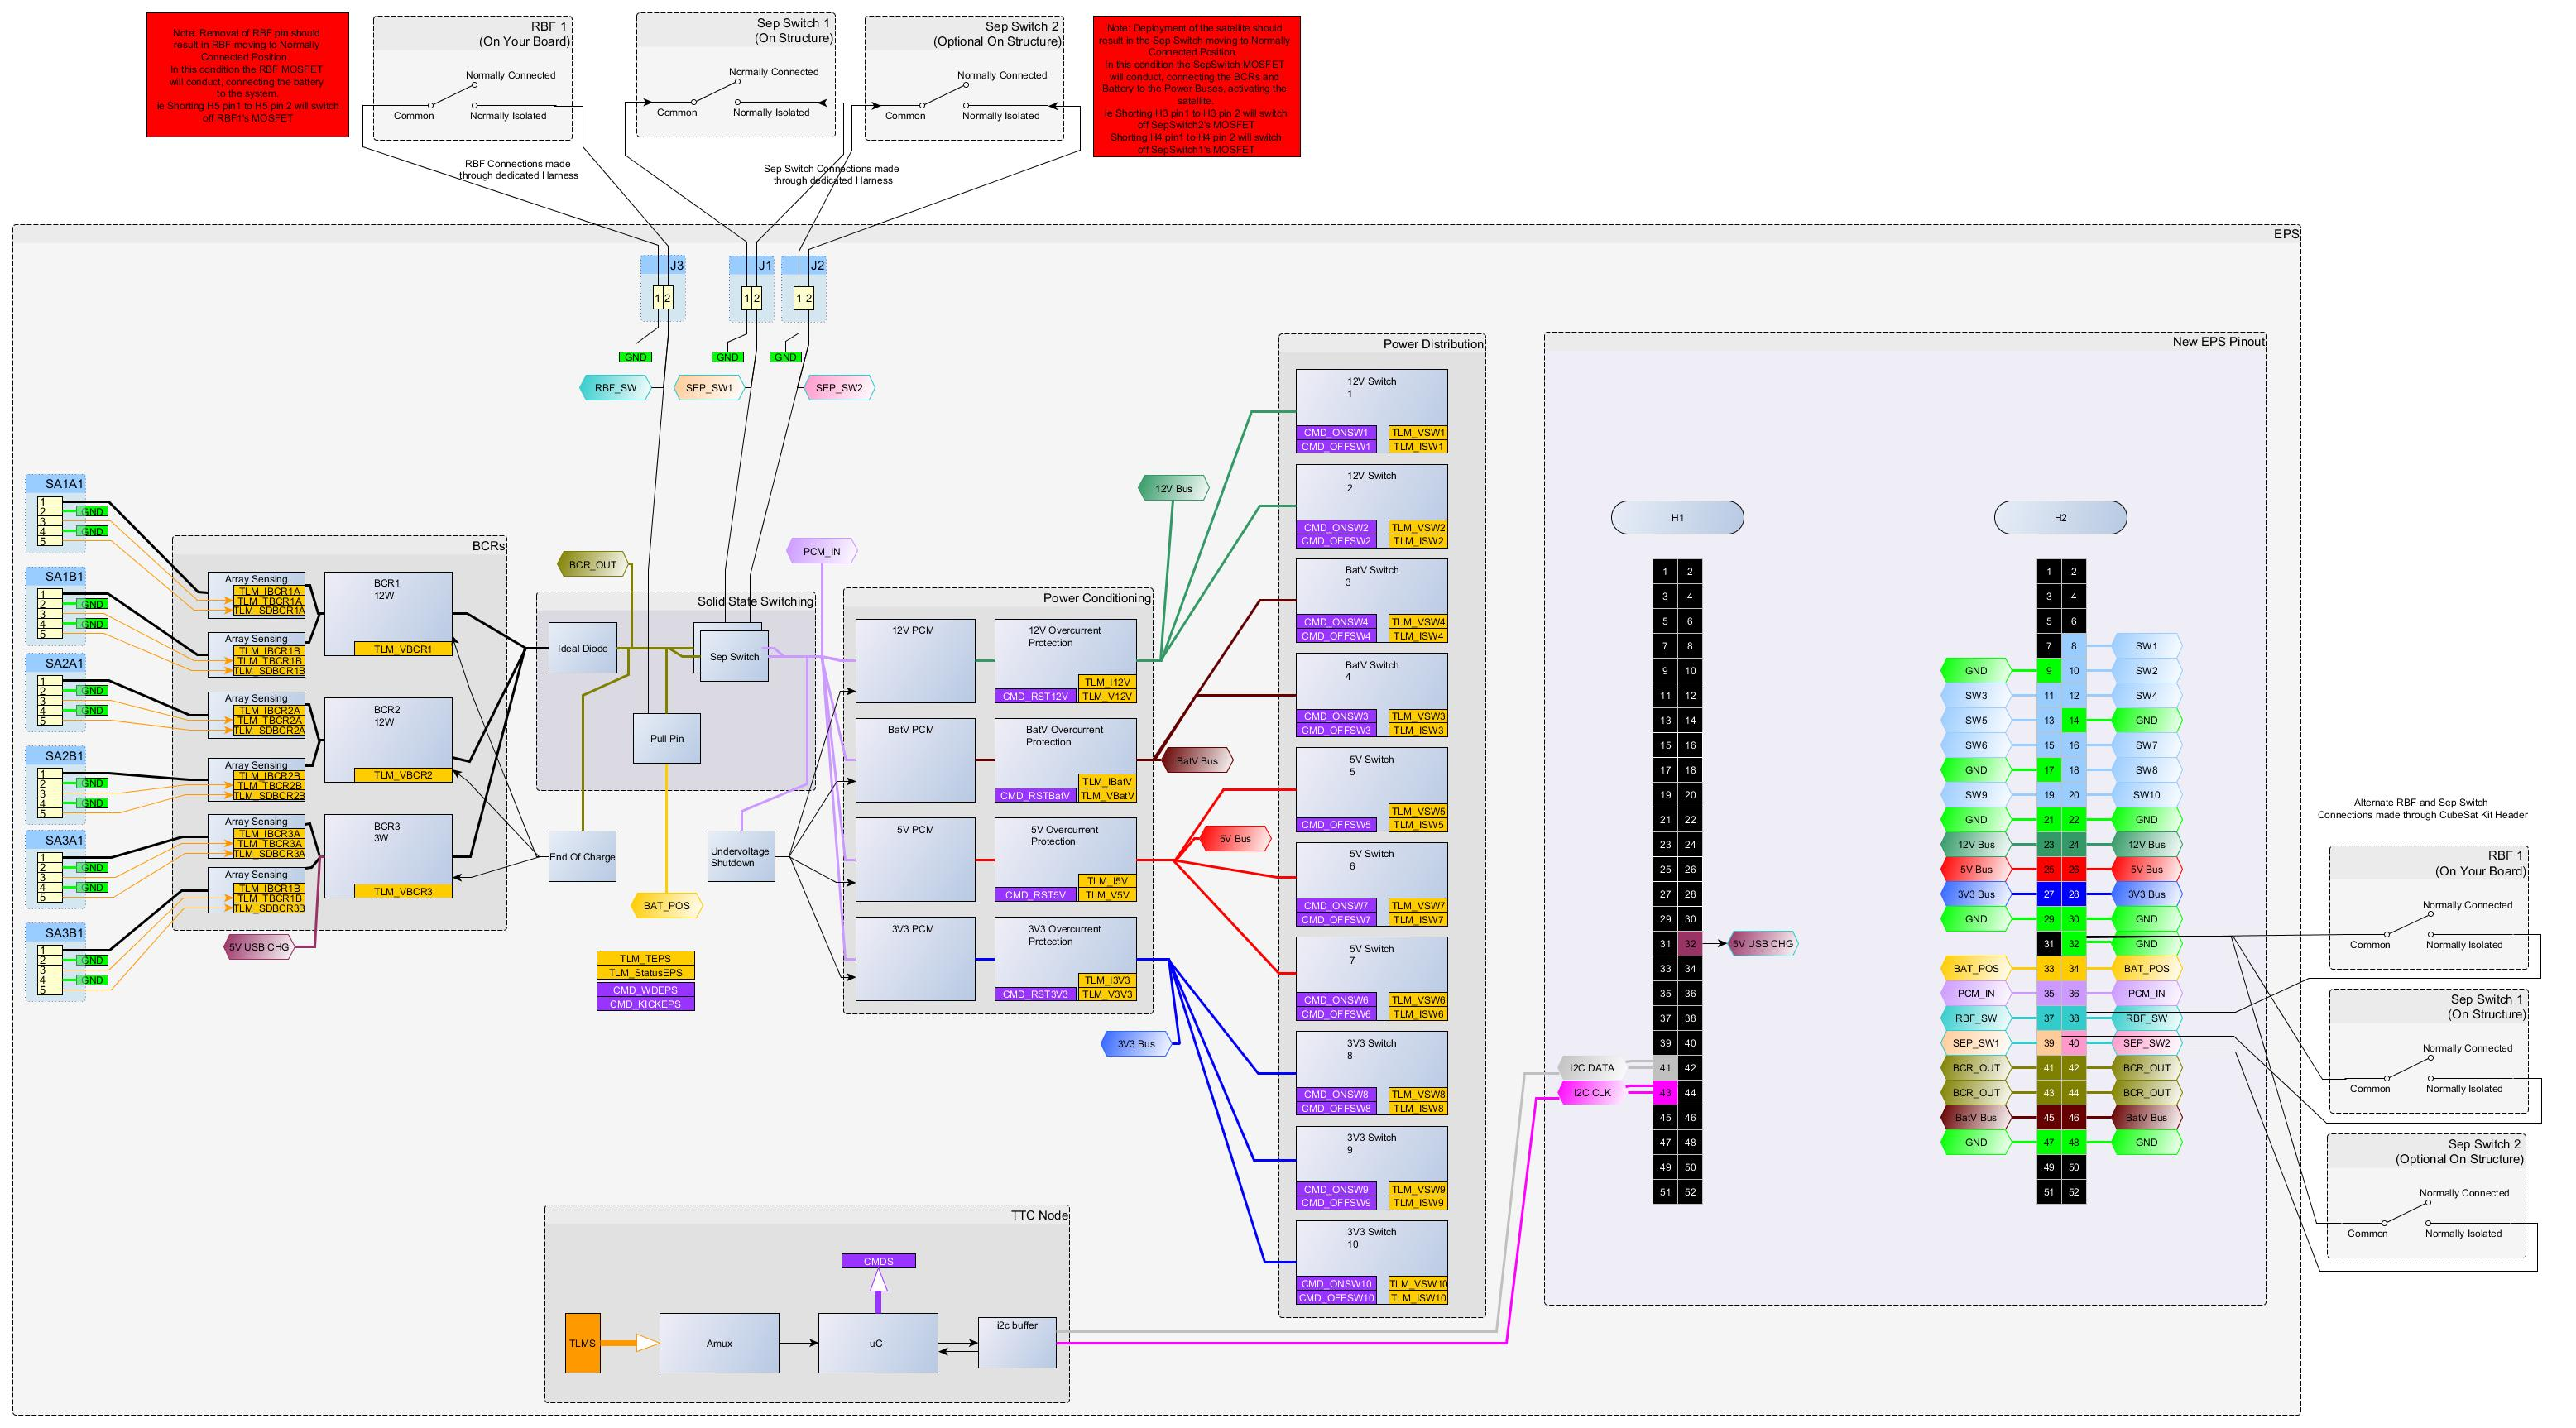
\includegraphics[width=0.9\linewidth]{./03/fig/eps_bd.jpg}
	\caption{Functional Diagram of EPS \cite{eps_um}}
	\label{fig3-1_eps_bd}
\end{figure}
\end{landscape}
\subsection{ミッション部電源系}
ミッション部電源系はOBCが送信したUART信号によりRaspberry PiがスイッチのON/OFFを切り替えることで操作される.詳細は\verb|\ref{text}|で述べる.
\subsection{電源系コメント}

\subsubsection{SAP}
\paragraph{SAP製作}
\begin{itemize}
	\item SAP製作及びSAP試験は作業量的には1人いれば十分可能だが,精神衛生上2人以上での作業を勧める.特にSAP出力特性試験では連日3号館101室を真っ暗にして何時間も1人での作業が続き,思っていた以上に負担が大きかった.
	\item SAP製作は非常に時間がかかる上に少しのミスで大きな手戻りが発生する作業である.購入するセル枚数,製作時間には大きくマージンをとっておくことを推奨する.OrigamiSat-1では最終的にFM機体用のセルの予備がなくなり,一部表面にひびが入っているセルを使用することになった.なお,OrigamiSat-1の試験においては,多少表面にひびが入っていても太陽電池の出力に変化はみられなかった.しかし軌道上での耐久性等に影響が出ることも考えられる.製作時間に関しては,アレイ化の作業時間に加えて,接着剤の乾燥時間も必要であるため,1回手戻りが発生すると2週間弱追加でかかった.
	\item 土台への接着後,アレイのうち1つでもセルが破損した場合,基本的にはアレイ全て取り換える必要がある.なお,一部のみの取り換えは不可能ではない.実際OrigamiSat-1では予備のセルがなかったこともあり,開発過程で4直のアレイのうち1枚だけを取り除いて他のセルを再利用したこともある.しかし取り換え作業は非常に困難な上,正常な他のセルも傷つける可能性が高い.
	\item OrigamiSat-1では太陽電池セルの総枚数が18枚であったためSAP製作が可能であったが,今後の衛星開発でもし太陽電池の枚数を増やすことがあれば,予算との兼ね合いもあるが,SAP製作の外注も検討するべきだと思う.SAPの設計次第ではあるが,太陽電池のセル単位の購入ではなくアレイ化までしてもらった状態での購入も選択肢として存在する.BBMからFMまでで合計何枚の太陽電池セルを発注するか,SAPの製作精度,開発時間等を含めSAP製作のどこを自分達で行うか今後の衛星開発では検討することを勧める.
	\item 内之浦でのOrigamiSat-1のE-SSODへの挿入時,IAの点検担当の方から感光基板の端のわずかな浮きを指摘された.この浮きは接着作業が完璧でなかったことが原因で生じたものであり,衛星引き渡し時は,振動等によってこれ以上浮きが進展しないことを説明し理解が得られた.このような浮きが生じないようにするためには,接着作業だけでなく乾燥期間の重し等の状態にも注意が必要である.
\end{itemize}
\paragraph{SAP試験}
\begin{itemize}
	\item 出力特性試験では,あらかじめ大きなブレッドボード上に試験に使う抵抗を一式用意しておき,ハーネスの接続先を変えるだけの状態で試験をした方がよかった.FM用SAP試験では,残り作業量がわずかだと思っていたため毎回抵抗を付け替えて行っていたが,1回の試験での付け替えには時間がかかる上に,最終的には何かと追加試験をやる機会が増えたため,改善しておけばよかった.
	\item 太陽シミュレーター及びサーモパイル(太陽シミュレーター用放射強度計)は非常に高価な機器であるため,取り扱いには特に注意する.また,サーモパイルの管理には注意をすること.一時期サーモパイルが行方不明になっていたようであるが,サーモパイルがなければ正しく放射強度の設定を行うことができず試験にならないため要注意.また,松永研所有の機器であるため,使用許可を必ずとること.使用報告の徹底が行き届いておらず,松永先生に注意されたことがあった.
\end{itemize}
\section{通信系 (衛星) (大本)}

本衛星に搭載する通信機としては,以下の3つがある.
\begin{itemize}
	\item {1} 地上局からのアップリンクを受信するVHF系
	\item {2} 地上局へCW信号,FM信号をダウンリンクするUHF系
	\item {3} 地上局へ大容量データをダウンリンクする5.8GHz系
\end{itemize}

衛星と地上局の通信の概略図を図\ref{fig4-2-1}に示す.
本衛星の回線設計は本衛星の軌道情報,東工大松永研究室地上局設備の性能を加味し,図\ref{fig4-2-2}のようになされた.
それぞれに要求される性能を記述する.
\begin{figure}[H]
	\centering
	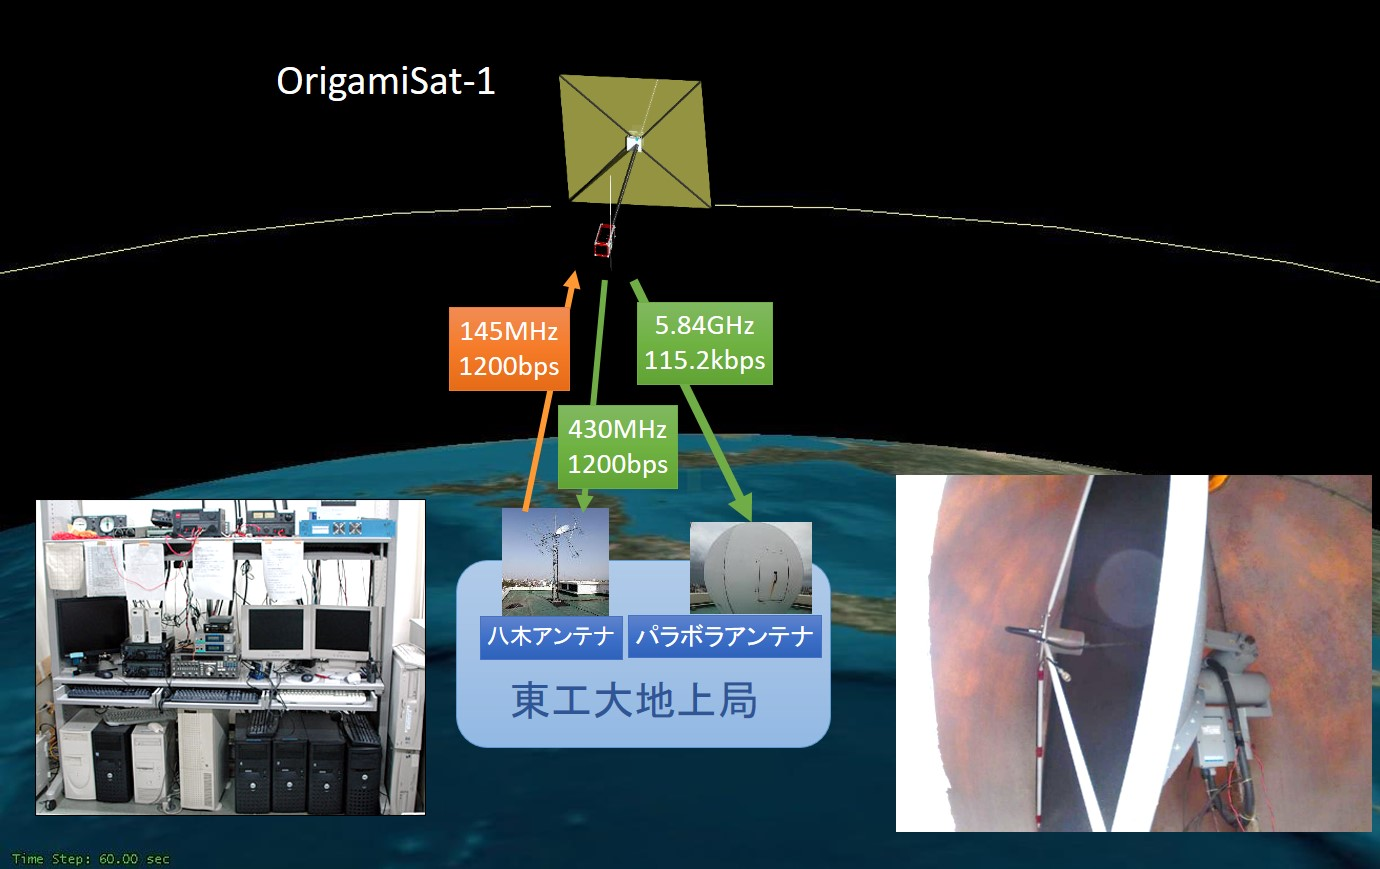
\includegraphics[scale=0.5]{03/fig/4-2-1.jpg}
	\caption{通信系概略図}
	\label{fig4-2-1}
\end{figure}
\begin{figure}[H]
	\centering
	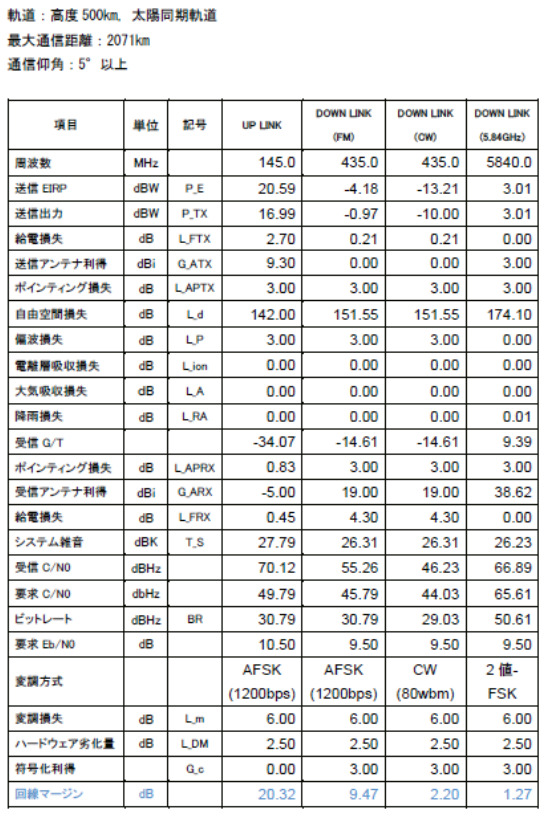
\includegraphics[scale=0.4]{03/fig/4-2-2.jpg}
	\caption{回線設計}
	\label{fig4-2-2}
\end{figure}

\subsection{VHF系}
VHF帯(Very High Frequency)の通信機では地上局からのアップリンクを受信するために用いる.通信機は西無線研究所の301A型を用いた.
アンテナにはコンベックス加工を行ったリン青銅製のモノポールアンテナ(幅5mm, 厚さ0.1mm)のものを用い,長さはインピーダンスマッチング試験を通じて決定した.
以下に設計スペックおよび系統図(\ref{fig4-2-3})を示す.
\begin{itemize}
	\item 周波数:145.980MHz
	\item 送信出力:100mW(CW),800mW(CW)
	\item 寸法:60x50x10.5mm
	\item 重量:38g
	\item アンテナ利得:0dBi
	\item 周波数帯域幅:500Hz(CW),20kHz(FM)
\end{itemize}
\begin{figure}[H]
	\centering
	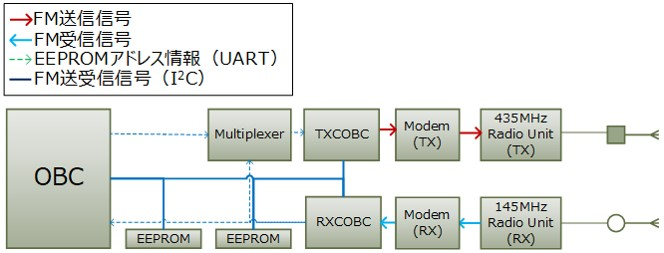
\includegraphics[scale=0.6]{03/fig/4-2-3.jpg}
	\caption{UHF/VHF系通信系統図}
	\label{fig4-2-3}
\end{figure}

\subsection{UHF系}
UHF帯(Ultra High Frequency)の通信機では地上局へCW信号,FM信号をダウンリンクするために用いる.通信機は西無線研究所の301A型を用いた.
アンテナにはコンベックス加工を行ったリン青銅のモノポールアンテナ(幅5mm, 厚さ0.1mm)のものを用い,長さはインピーダンスマッチング試験を通じて決定した.
以下に設計スペックおよび系統図(\ref{fig4-2-3})を示す.
\begin{itemize}
	\item 周波数:437.505MHz
	\item 寸法:100x60x10.5mm
	\item 重量:60g
	\item アンテナ利得:0dBi
\end{itemize}

\subsection{5.8GHz系}
5.8GHz系の通信機では画像などの大容量データをダウンリンクするために用いる.通信機はロジカルプロダクト社製 LPTX5840-1を用いた.
アンテナには円偏波パッチアンテナ(30x30x1.6mm)を用いた.
以下に設計スペックおよび系統図(\ref{fig4-2-4})を示す.
\begin{itemize}
	\item 周波数:5840MHz
	\item 送信出力:2W
	\item 寸法:76x70x16mm
	\item 重量:220g
	\item アンテナ利得:3dBi
	\item 周波数帯域幅:210kHz
\end{itemize}
\begin{figure}[H]
	\centering
	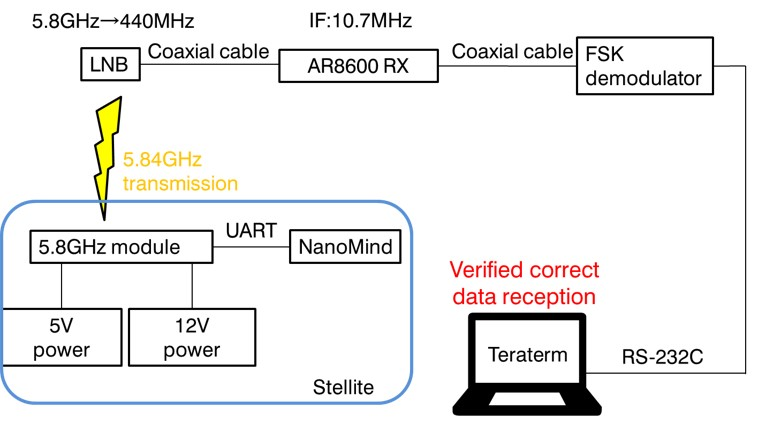
\includegraphics[scale=0.6]{03/fig/4-2-4.jpg}
	\caption{5.84GHz系通信系統図}
	\label{fig4-2-4}
\end{figure}

\section{地上局(加藤・飯島)}
\section{C\&DH系(OBC 岩崎・小出・林・井手, COBC 黒崎・中塚・大本, Rpi 飯島)}
%ソフトウェア設計思想
%HKデータ
%コマンド予約・実行
%機能確認
%文責:中塚・黒崎

\subsection{CIB}
\subsubsection{基本設計思想}
CIB(Communication and Inhibit Board)は,イプシロンロケット搭載のためのシステム安全要求(電源のインヒビット機能)を満たすこと,および消費電力の高い5.8GHz送信機の電源系統を別とすることを目的として新規開発を行った基板であり,バッテリとEPSの間に挿入されている.また,VHF/UHFの受信機(RX)/送信機(TX)(西無線301A型)のためのマイコンであるRXPIC(PIC 16F877A),TXPIC(PIC 16F886)およびモデム回路もCIB上に搭載されている.RXPICはメインOBCより上位にあるものと考え,メインOBCを監視する.RXPIC及びTXPICはWDT(Watch Dog Timer)を用いて異常時には自身へリセットをかける.

\subsubsection{プログラム概要}
\paragraph{RXPIC役割}\label{par:RXPIC役割}
RXPICの持つ主要機能は大きく分けて以下のものがある.RXPICの各機能詳細は\ref{subsubsec:RXPIC詳細}参照.
\begin{itemize}
	\item 初期運用
	\item EPSリセット
	\item 無線機の周波数設定
	\item バッテリ電圧測定及び衛星モード切替
	\item アップリンクコマンド処理
\end{itemize}

\paragraph{TXPIC役割}\label{par:TXPIC役割}
TXPICの持つ主要機能は大きく分けて以下のものがある.TXPICの各機能詳細は\ref{subsubsec:TXPIC詳細}参照.
\begin{itemize}
	\item 初期運用
	\item ADCの値を取得
	\item レシーブコマンドダウンリンク
	\item CWダウンリンク(HKデータ/指定データ)
	\item FMダウンリンク(HKデータ/指定データ)
	\item スイッチ操作
\end{itemize}

\subsubsection{RXPIC詳細}\label{subsubsec:RXPIC詳細}
RXPICのフローチャートを図\ref{fig:3-4-2-1}に示す.
\begin{figure}[H]
	\centering
	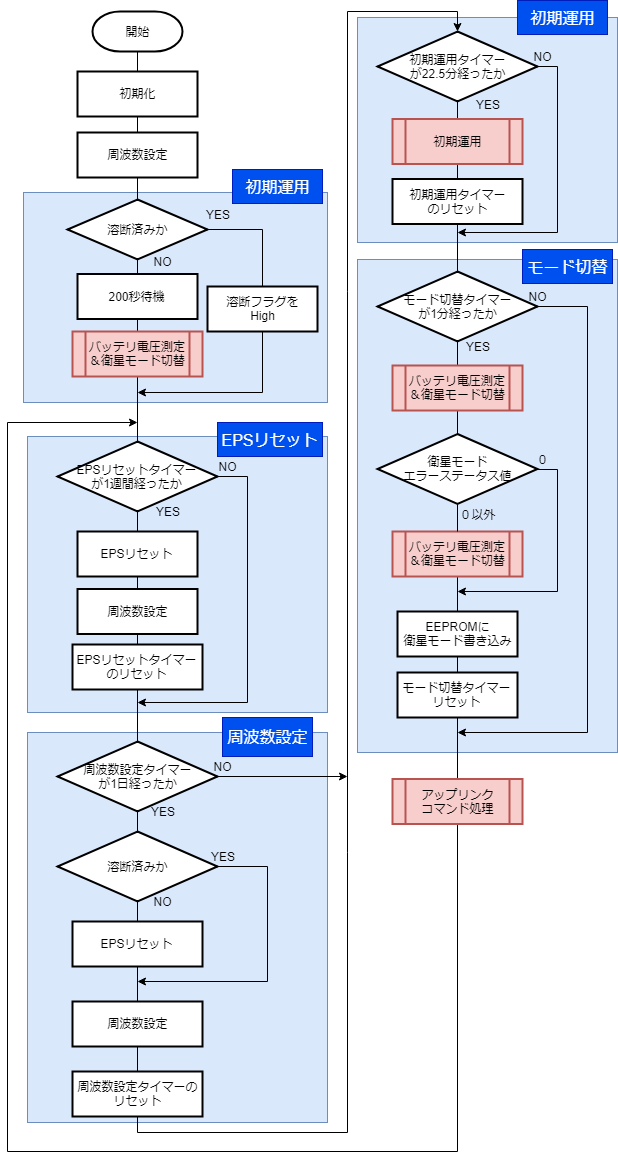
\includegraphics[scale=0.5]{03/fig/3-4-2-1.png}
	\caption{RXPIC全体フローチャート}
	\label{fig:3-4-2-1}
\end{figure}
以下でRXPICの各機能について説明する.
\paragraph{初期運用}
詳細については初期運用項(統合時ラベル付けして参照)を参照.

\paragraph{EPSリセット}
RXPICでは1週間毎にEPSリセットのタイマー割込みが発生する.これはRXPIC及びTXPIC以外の,EPSから電源供給されているコンポーネントの不具合が生じ,実装しているエラー処理で対応しきれないケースに備え,1週間毎にリセットをかけることを目的として実装した機能である.なお初期運用中は,これに加えて1日毎のEPSリセットも行われる.

\paragraph{無線機の周波数設定}
RXPICでは1日毎に無線機の周波数設定のタイマー割込みが発生する.無線機の周波数設定でエラーが生じ通信できなくなるケースに備え,通常の無線機の電源ON/OFFに伴う周波数設定とは別に実装した機能である.

\paragraph{バッテリ電圧測定及び衛星モード切替}
RXPICでは1分毎にバッテリ電圧測定及び衛星モード切替のためのタイマー割込みが発生する.バッテリ電圧に応じて衛星モードはNominal,Saving,Survivalに切り替わり,モードに応じてアクティブなコンポーネントが変化する.モード切替の概念を図\ref{fig:3-4-2-2}に示す.モード切替の閾値電圧の初期値はそれぞれ図\ref{fig:3-4-2-2}に示す値であり,これらの閾値はコマンドにより変更することができる.電圧降下時と上昇時の初期閾値電圧に差があるのは,電圧上昇によるモード切替に伴いアクティブなコンポーネントが増えることで一時的に電圧が降下し,直後に再びモード切替が起こることを防ぐためである.
\begin{figure}[H]
	\centering
	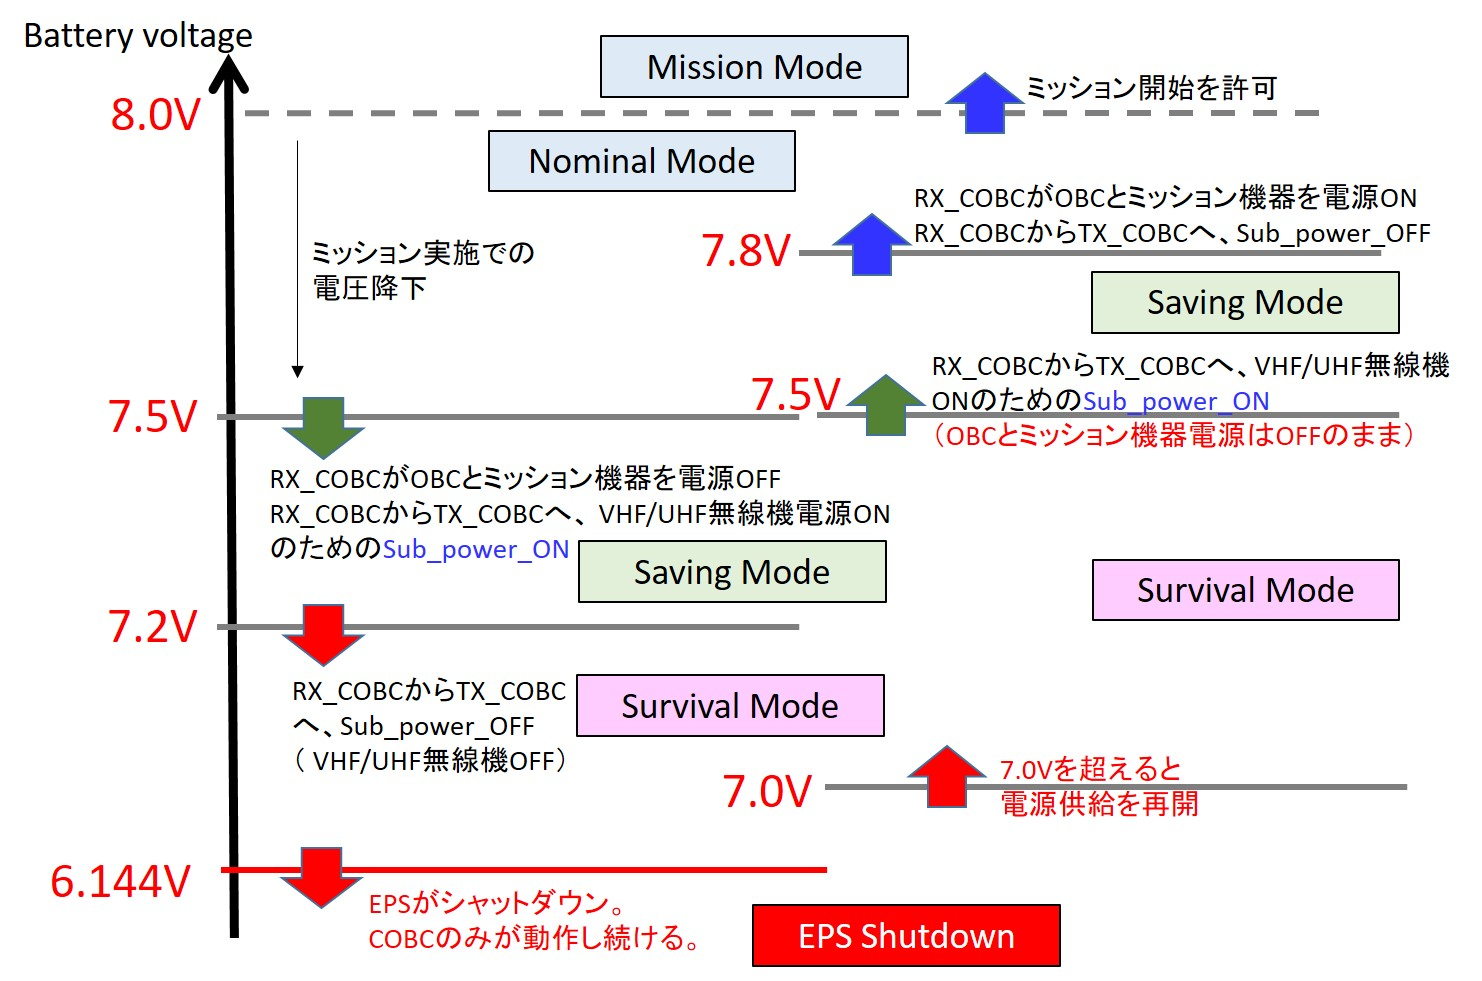
\includegraphics[scale=0.6]{03/fig/3-4-2-2.jpg}
	\caption{モード切替の概念図}
	\label{fig:3-4-2-2}
\end{figure}
バッテリ電圧測定及び衛星モード切替のフローチャートを図\ref{fig:3-4-2-3}に示す.
衛星モード切替では,バッテリー電圧,閾値電圧,及び前の衛星モードを取得し,それを元に切替処理を行っている.閾値電圧はメイン/サブEEPROMを,前の衛星モードはメイン/サブEEPROM及びグローバル変数を利用して,取得できないリスクを低減させている.また衛星モード切替中にエラーが生じ,正常に処理が完了できない場合には基本的にSavingモードに切り替える.
バッテリ電圧測定及び衛星モード切替処理では返り値として1byteのエラーステータスを用意しており,異なる2bitずつを異なるエラーに割り当てることで,同時に生じる複数のエラーを検知できるように実装している.1bitずつの割り当てでないのは,放射線等によるbit反転の影響を小さくするためである.エラー値の詳細についてはOP-S1-0109「CW通信フォーマット」の衛星モードエラーステータスを参照.また衛星モード切替の詳細については,OP-S1-0104「OrigamiSat-1 モード切替について」を参照.
\begin{figure}[H]
	\centering
	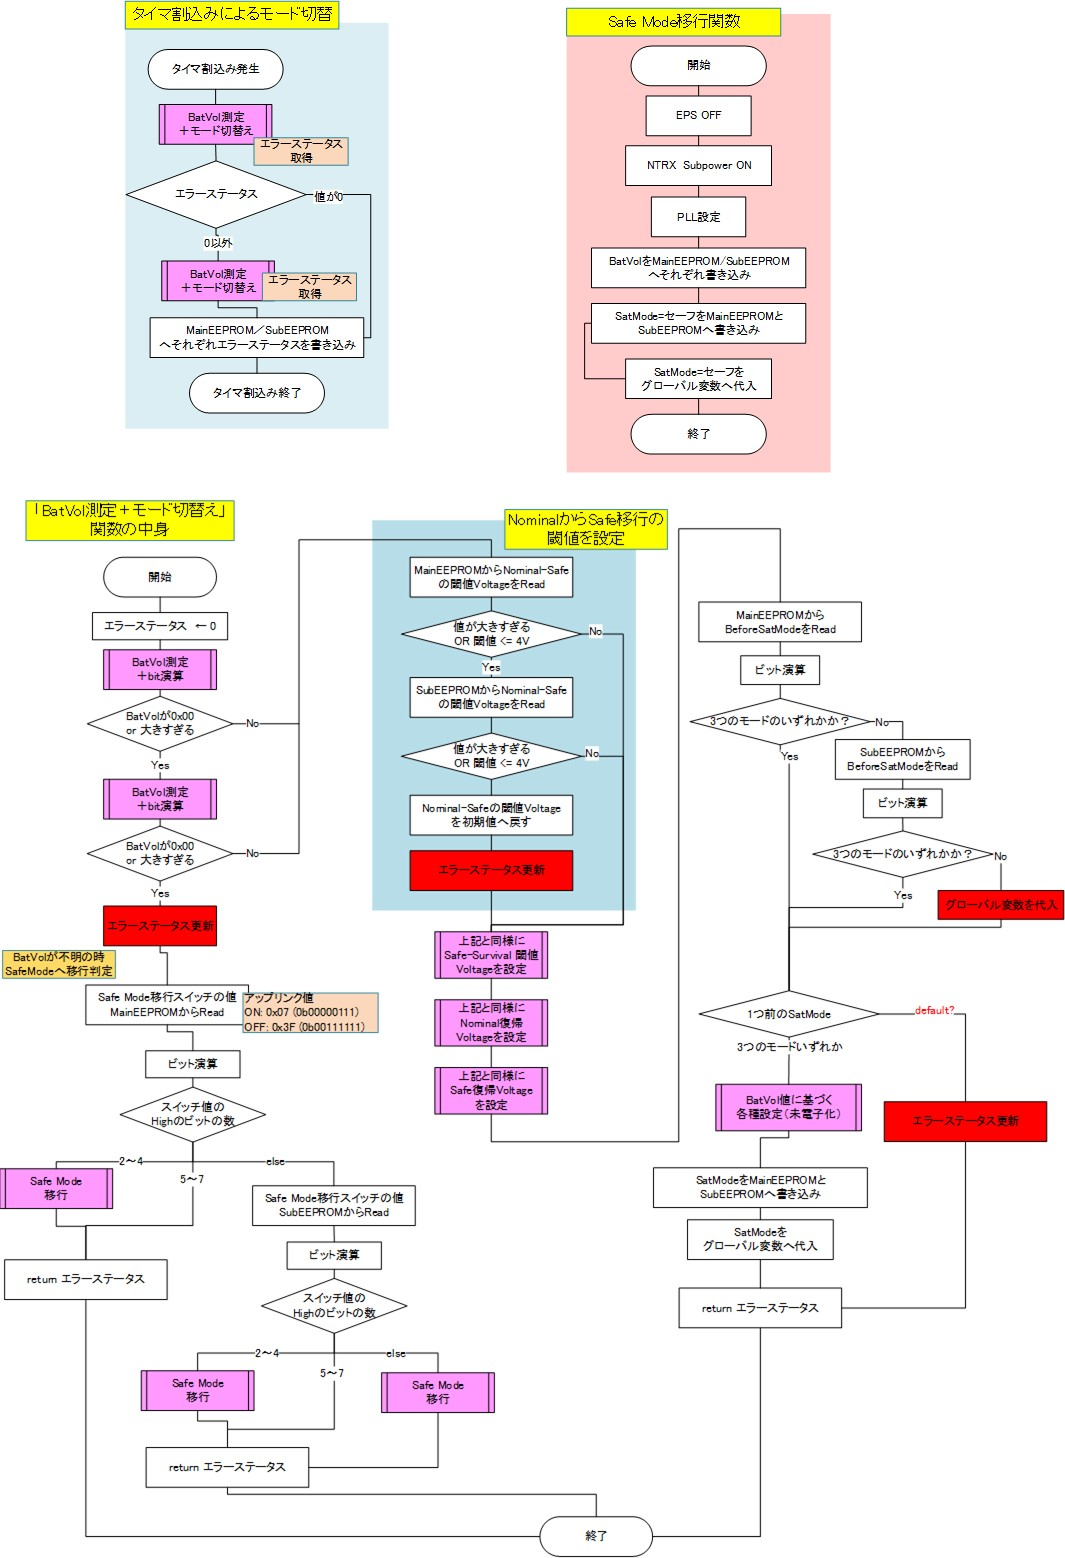
\includegraphics[scale=0.9]{03/fig/3-4-2-3.jpg}
	\caption{モード切替フローチャート}
	\label{fig:3-4-2-3}
\end{figure}

\paragraph{アップリンクコマンド処理}
RXPICのアップリンクコマンド処理時のフローチャートを図\ref{fig:3-4-2-4}に示す.地上局からのアップリンクコマンドを受信後コマンドIDの確認を行い,最終実行コマンドIDと同じであればコマンドの実行は行わない.これは地上局から誤って同じコマンドを2回送った時,衛星がそれを実行しないようにするためである.コマンドIDのチェックが終わった後はEEPROMにコマンドを書き込み,コマンドターゲットに応じて処理を行う.コマンドターゲットがRXPICであった場合のコマンド実行関数内では,コマンドタイプに応じてswitch文で分岐し,それぞれの処理を行っている.
\begin{figure}[H]
	\centering
	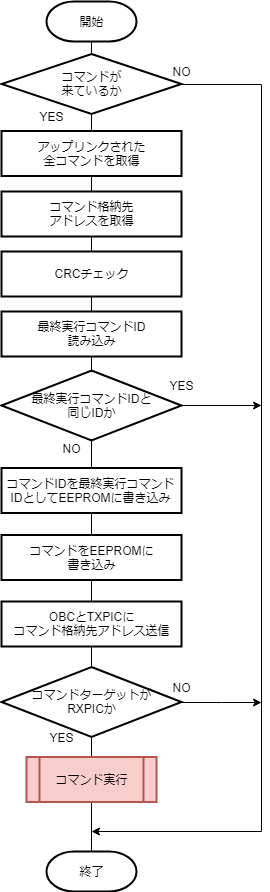
\includegraphics[scale=0.6]{03/fig/3-4-2-4.png}
	\caption{アップリンクコマンド処理フローチャート}
	\label{fig:3-4-2-4}
\end{figure}

\subsubsection{TXPIC詳細}\label{subsubsec:TXPIC詳細}
TXPICのフローチャートを図\ref{fig:3-4-2-5}に示す.図\ref{fig:3-4-2-5}のフローチャートとは別に割込み関数として,コマンドが来た際に
\ref{par:TXPIC役割}の主要機能のうち,レシーブコマンドダウンリンク,CWダウンリンク(データ),FMダウンリンク(HK/データ),スイッチ切替は,図\ref{fig:3-4-2-5}中のコマンド実行関数内で行われる.
\begin{figure}[H]
	\centering
	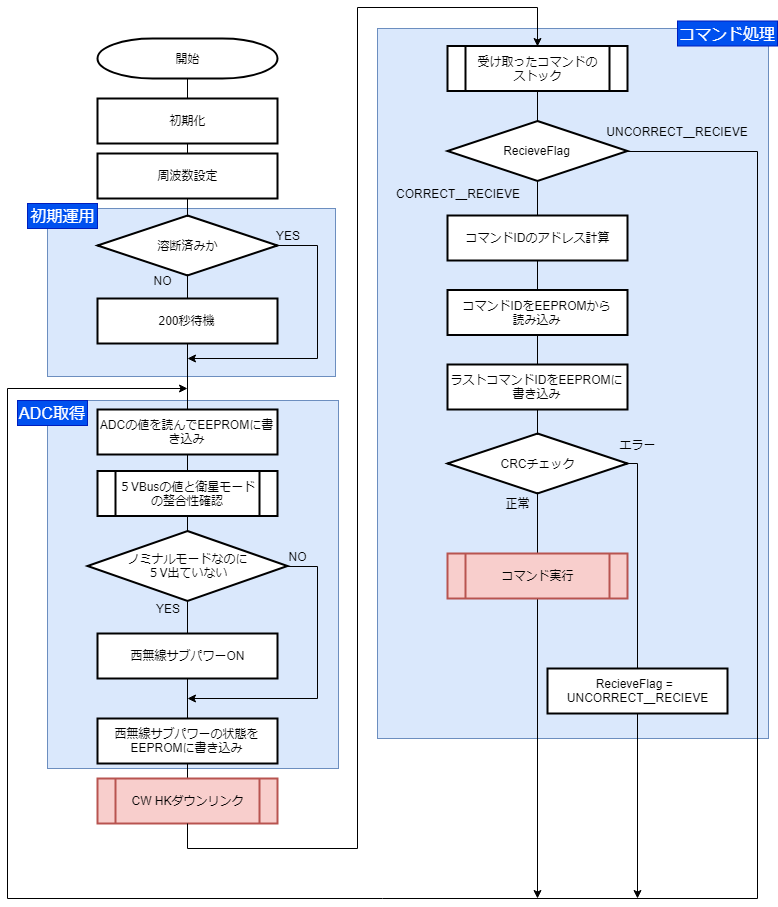
\includegraphics[scale=0.6]{03/fig/3-4-2-5.png}
	\caption{TXPIC全体フローチャート}
	\label{fig:3-4-2-5}
\end{figure}
以下でTXPICの各機能について説明する.

\paragraph{初期運用}
詳細については初期運用項(統合時ラベル付けして参照)を参照.

\paragraph{ADCの値を取得}
ADCのCH1-4の値を取得し,EEPROMに保存する.なお,CH1-4はそれぞれバッテリ温度,EPS5Vライン電圧,EPS3.3Vライン電圧,5Vライン電圧電圧の値を示す.ADCの値を取得後,EEPROMから衛星モードの読み込みを行い整合性を確認する.整合性がとれない,すなわちノミナルモードにもかかわらずEPS5Vラインの電圧が低かった場合,西無線のサブパワーをONにする.これは,ノミナル時にエラー等により西無線の電源が遮断され,地上局との通信ができなくなるリスクの低減のために実装を行った.

\paragraph{レシーブコマンドダウンリンク}
地上局からアップリンクされたコマンドを受信した後,RXPICからの指示を受けてTXPICはアップリンクされたコマンドを地上局に返す.
これはコマンドアップリンク時,衛星側がコマンドを受け取ったかどうか判断するために実装を行った.

\paragraph{CW ダウンリンク}
CWダウンリンクは,HKダウンリンクとコマンドによる指定データのダウンリンクの2種類がある.
CWHKダウンリンクフォーマットの詳細については,OP-S1-0109「CW通信フォーマット」を参照.
コマンドによる指定データのダウンリンクでは,コマンドによって指定されたEEPROMアドレスのデータを指定回数ダウンリンクする.CWによるデータダウンリンク機能は,FM及び5.8GHzデータ送信機能が共に失われた場合に備え実装を行った.

\paragraph{FMダウンリンク}
FMダウンリンクは,HKダウンリンクとコマンドによる指定データのダウンリンクの2種類がある.
FMダウンリンクフォーマットの詳細については,OP-S1-0108「FMダウンリンクフォーマット」を参照.

\paragraph{スイッチ切替}
コマンドに応じてヒーター,送受信機,5.8GHz送信機予備電源,溶断回路,WDT,FMPTT,CWKEYのON/OFFを切り替える.コマンドで時間を指定することにより,指定時間ON/OFFを切り替えた後,元の状態に戻す機能が実装されている.

\subsubsection{コメントや次回への改善点}
\begin{itemize}
	\item システム設計を早い時期にしっかり行い,優先順位の高いものからプログラムを作っていくべきだった.複数個所で使う重要な機能の開発が後半に残っていたことがあった.また,機能を実装したものの結局使わないものや,ほぼ同じ機能を持つ関数が複数存在する事態が開発途中で発生した.またOrigamiSat-1のCIBでは開発の遅れからエラー処理を実装しきれないところが多かった.システム設計を早期にしっかり行い,エラーについても体系的に処理を行いHKデータ等でダウンリンクすることで,エラー箇所の切り分けを行うことができれば故障解析もしやすくなったのではないかと思う.
	\item EPSリセットの1週間という頻度には根拠がないため,次回の衛星開発においてはリセット頻度を検討する必要がある.また,OrigamiSat-1ではRX/TXPICは自身で定期的にリセットをすることはなかったが,これらについても定期的なリセット機能をつけた方がよかった可能性もある.
	\item CW HKデータに衛星モード切替のエラーステータスを含めたのは良かった.当初の予定では含まれておらず,衛星引き渡し直前にCW HKデータのうちTX/RXコマンドエラーステータス機能にバグを発見しFM機への実装を断念したことを受け,CIB開発メンバーで相談し急遽HKデータに入れたものであるが,結果的に衛星の状況を確認し故障解析に必要なデータとして役立った.
	\item CW HKダウンリンクでは,データ1つずつEEPROMを読みにいく処理を行っていたが,結果的にEEPROMを読みにいく頻度が高くなり,I2Cエラーの一因となっていた可能性がある.複数データをまとめて読みにいく処理に変えるという案も開発途中出ていたが,開発期が間に合わなかった.また,他のコンポーネントがEEPROMを読んでいる時は待機するような機能を実装した方がよかった.
	\item 複数の同一基板を用意しておいた方がよかった.FM機搭載基板と全く同じ基板が試験用に存在しなかったため,環境が異なっていたことにより,打ち上げ前に発見できなかったバグが存在した.特に周波数設定に関しては,EMでは西無線のテストボードを使用していたためFM機体の試験環境とは大きく異なっていた.
	
\end{itemize}

%文責:小出,林,岩崎,井手

\subsection{OBC}
\subsubsection{概要および設計思想(林)}
\begin{itemize}
	\item ここにOBCの概要を書く
\end{itemize}
\subsubsection{OBCの内部処理}
\textbf{OBC内部処理の全体像(林)}\par
\begin{itemize}
	\item OBCの内部処理に関して具体的にかく
	\item コマンド受信とHK受信などの詳細は書かずに全体像のみをここではじめに書く
\end{itemize}
\textbf{初期運用(小出)}\par
\textbf{HK生成(小出)}\par
\textbf{コマンド受信(林)}\par
\subsubsection{開発中における不具合およびトラブル(小出・林)}
\subsubsection{次回への改善点(小出・林)}

%文責:黒崎・小出
%***各項目の執筆担当者名は最後に消してください

\subsection{初期運用}
%画像のファイル名は「3-4-Ini-1.jpg」「3-4-Ini-2.jpg」...
%ラベル名は「fig3-4-Ini-1」「fig3-4-Ini-2」...

\subsubsection{初期運用概要(黒崎)}
初期運用では,放出直後に地上との通信を行うため,アンテナの展開を試みるフェーズである.アンテナを収納する際に巻かれたテグスを溶断することでアンテナの展開を行う.以下に初期運用の簡単な流れを示す.

\begin{itemize}
	\item[1] OBCまたはCOBCが溶断する
	\item[2] 溶断が完了しアンテナが展開し,CW HKダウンリンクが開始する
	\item[3] CW HKダウンリンクが地上局で確認されたら,溶断停止コマンドを東工大地上局からアップリンクを行う
	\item[4] 衛星が溶断停止コマンドを受信したら,溶断を停止し,初期運用モードから定常運用モードに移行する
	\item[5] CW HKダウンリンクの溶断ステータスが溶断前から溶断済みに更新されていることを確認することで,衛星が定常運用モードに移行したことを地上局が認識する
\end{itemize}

\subsubsection{基本設計思想(黒崎・小出)}
\begin{itemize}
	\item \textbf{OBCがメインで溶断を行う.OBCが溶断に失敗している場合にCIBが溶断を行う.}本来であれば,SavingモードでOBCの電源が切られてしまうため,CIBがメインで溶断を行う方がシンプルな設計に出来た.しかし,CIBは初期運用以外の開発がかなり遅れていたため,初期運用のデバックに割ける時間が限られていること,またCIBに機能の集中を避けること,溶断の電源の供給の1つがOBCしか出来ないことなどを考慮し,OBCをメインにしたという背景がある.
	\item \textbf{溶断頻度は22.5分間隔.}これは地球1周を90分かけるOrigamiSat-1の軌道において,地球1周の間に4回溶断をトライする設計になっている.地球1周分を基準に考えているのは,日向,日陰条件で宇宙環境温度が異なり,溶断の成功確率に影響が出ることを考慮している.
	\item \textbf{1日の間で8回(地球2周分)溶断をトライした後は,溶断を行わず待機.}これはバッテリーを温存するためである.
\end{itemize}

\newpage
\subsubsection{開発の流れ(黒崎)}
開発の流れは以下の通りである.
\begin{itemize}
	\item[3-A] 不具合想定表作成
	\item[3-B] ソフトフローチャート作成
	\item[3-C] ソフト作成
	\item[3-D] デバック
	\item[3-E] フローチャートとソフトが対応しているか確認
	\item[3-F] OBC/CIB統合
	\item[3-G] 恒温槽試験で溶断時間の確認
	\item[3-H] FM最終確認
\end{itemize}

各工程の詳細を以下に示す.
\begin{itemize}
	\item[3-A] \textbf{不具合想定表作成}:不具合想定表は,「A)不具合原因表」と「B) 不具合対応表」からなる.
	
	A)不具合原因表は,電源系,通信系,その他の3種類に分けて作成した.実際に作成した表を表\ref{table3-4-Ini-0-a},表\ref{table3-4-Ini-0-b},表\ref{table3-4-Ini-0-c}に示す.表\ref{table3-4-Ini-0-a}に関しては,機器のトラブルによる再起動/電源オフだけでなく,モード切替による意図的な再起動/電源オフも想定している.
	
	B)不具合対応表は,各シークエンスにおいて,表\ref{table3-4-Ini-0-a},表\ref{table3-4-Ini-0-b},表\ref{table3-4-Ini-0-c}で想定された不具合が発生した場合の,1.対処法(どのように冗長系を組むか),2.デバックの際の検証方法を示している.OBC,RXPIC,TXPICそれぞれにおいて対応表を作成した.実際に作成した表を表\ref{table3-4-Ini-1},表\ref{table3-4-Ini-2},表\ref{table3-4-Ini-3}に示す.
	
	\newpage
	\begin{table}[H]
		\centering
		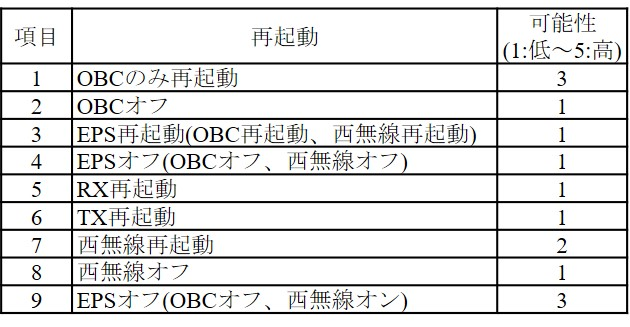
\includegraphics[scale=1]{03/fig/t3-4-Ini-0-a.jpg}
		\caption{不具合原因表(電源系)}
		\label{table3-4-Ini-0-a}
	\end{table}
	\begin{table}[H]
	\centering
	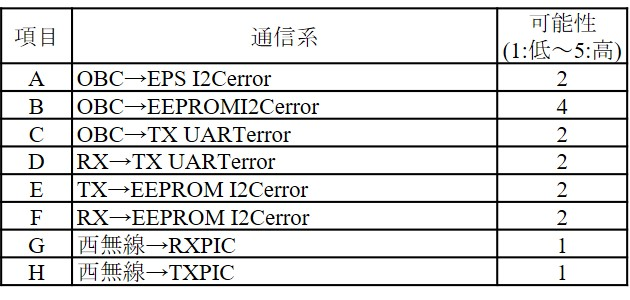
\includegraphics[scale=1]{03/fig/t3-4-Ini-0-b.jpg}
	\caption{不具合原因表(通信系)}
	\label{table3-4-Ini-0-b}
	\end{table}
	\begin{table}[H]
	\centering
	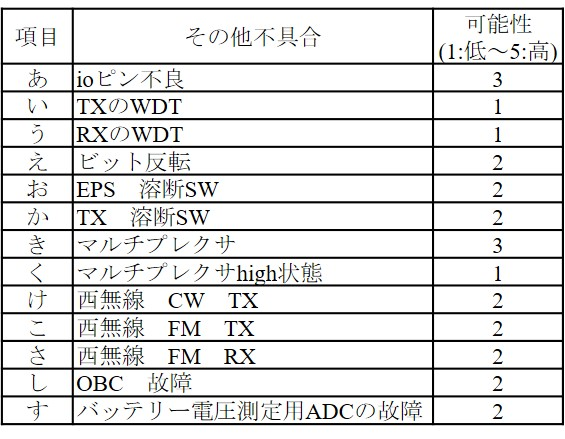
\includegraphics[scale=1]{03/fig/t3-4-Ini-0-c.jpg}
	\caption{不具合原因表(その他)}
	\label{table3-4-Ini-0-c}
	\end{table}
	\newpage
	
	\begin{table}[H]
		\centering
		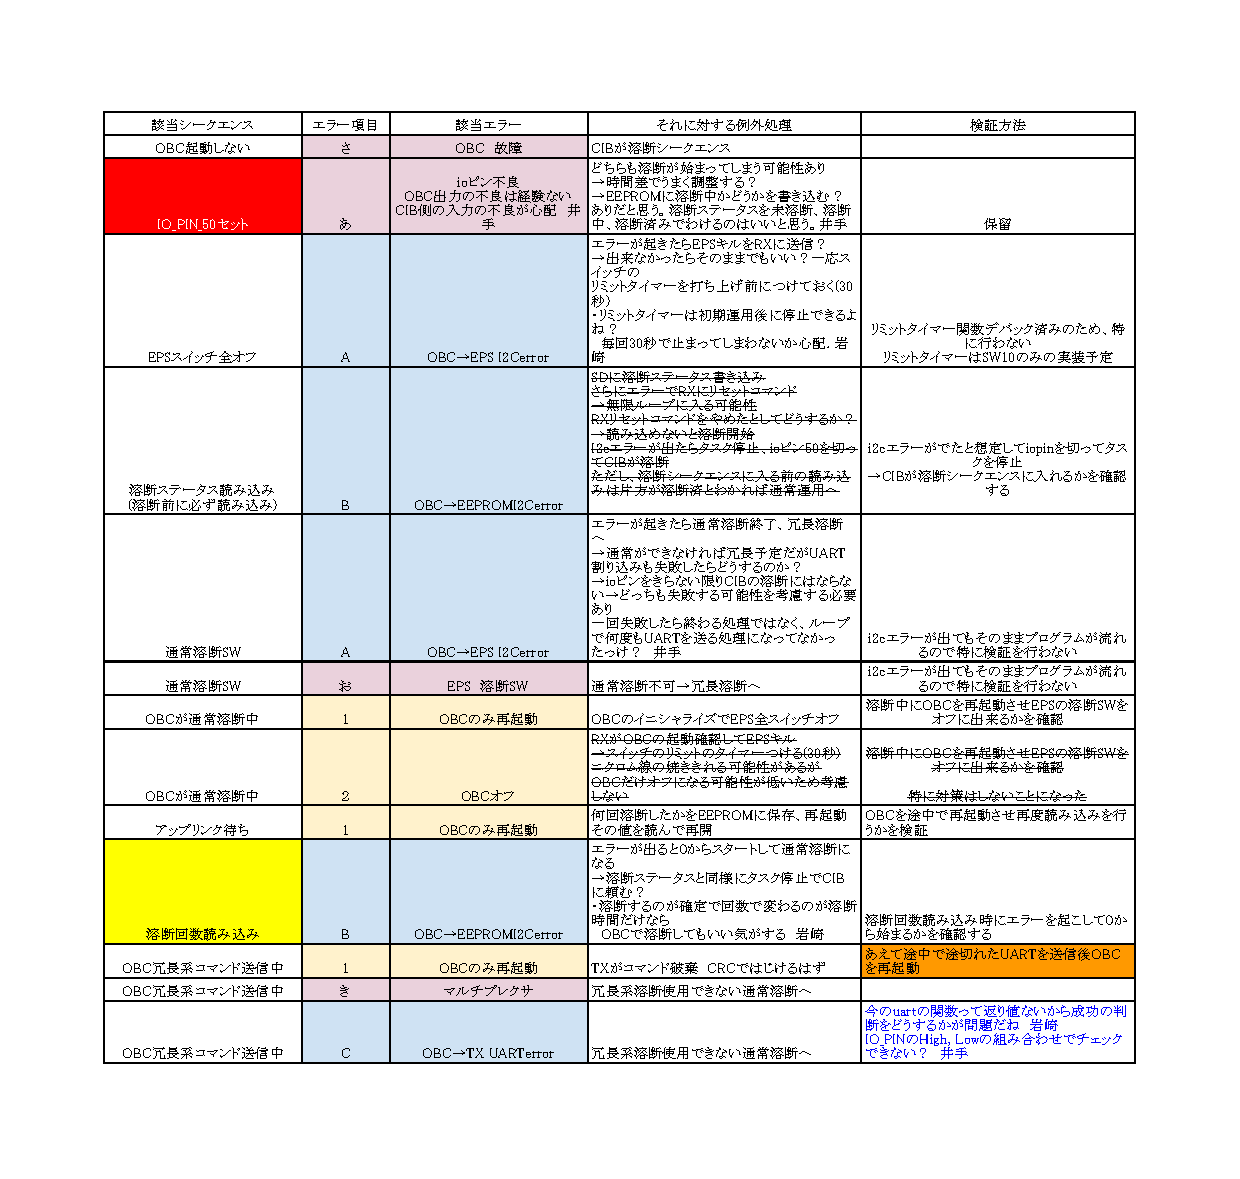
\includegraphics[scale=0.7]{03/fig/t3-4-Ini-1.pdf}
		\caption{不具合対応表(OBC)}
		\label{table3-4-Ini-1}
	\end{table}
	\begin{table}[H]
	\centering
	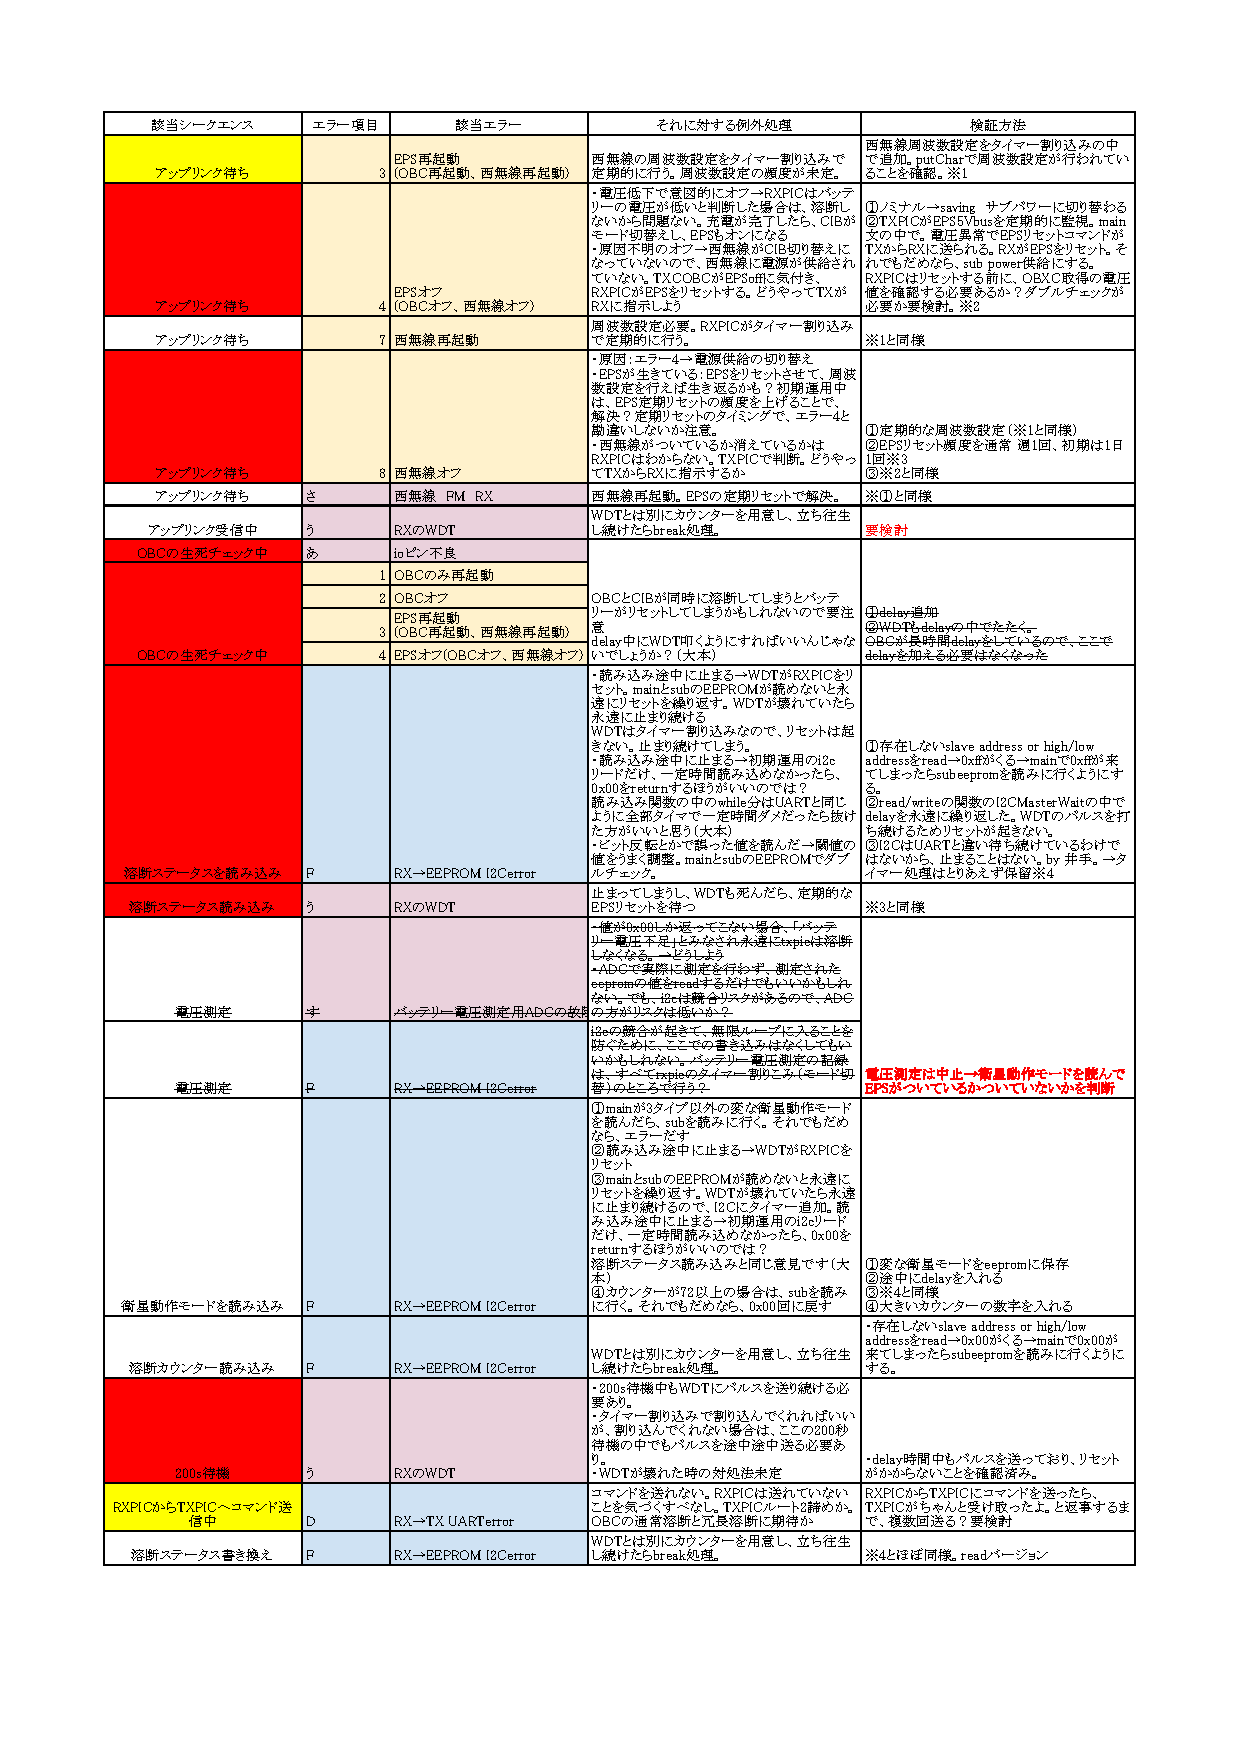
\includegraphics[scale=0.7]{03/fig/t3-4-Ini-2.pdf}
	\caption{不具合対応表(RXPIC)}
	\label{table3-4-Ini-2}
	\end{table}
	\begin{table}[H]
	\centering
	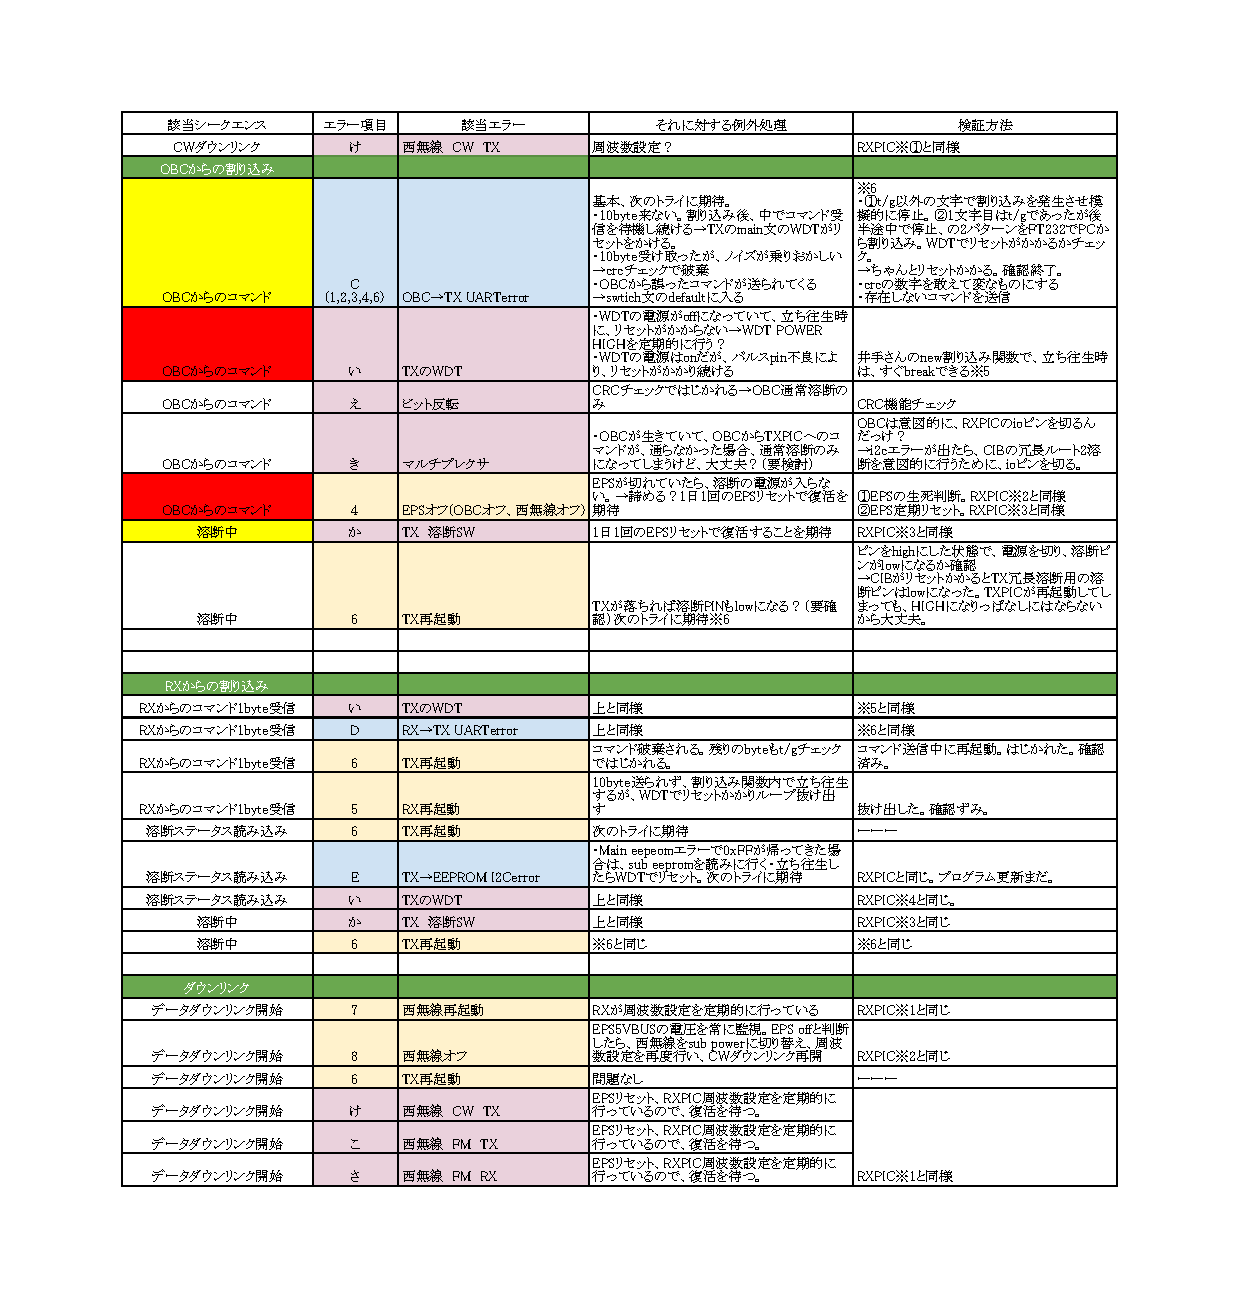
\includegraphics[scale=0.7]{03/fig/t3-4-Ini-3.pdf}
	\caption{不具合対応表(TXPIC)}
	\label{table3-4-Ini-3}
	\end{table}	

	%%%%%%%%%%%%%%%%%%%%%%%%%%
	\item[3-B] \textbf{ソフトフローチャート作成}:3-Aで作成した不具合想定表を元に,初期運用時のOBC,TXPIC,RXPICのフローチャートを作成した.作成したフローチャートは,他のコンポーネント担当者等とも検討した.
	
	\item[3-C] \textbf{ソフト作成}:3-Bで作成されたフローチャートを元に,ソフトを書いた.
	
	\item[3-D] \textbf{デバック}:3-Cと同時並行で書いたソフトをその都度デバックする.いつ,どの部分をデバックし,結果はどうであったかを必ず記録する.後に確認した際にどの部分までデバックしたか分からなくなってしまうため.
	
	\item[3-E] \textbf{フローチャートとソフトが対応しているか確認}
	\item[3-F] \textbf{OBC/CIB統合}.初期運用はOBCとCIBが連携して行うため,統合作業が必要である.冗長系を含むフローチャートの全てのルートにおいてバグが無いかを,単体では3-Dで確認済みだが,OBCとCIBのプログラムを同時に動かして確認した.
	\item[3-G] \textbf{恒温槽試験で溶断時間の確認}:恒温槽において,宇宙環境の想定最大温度50℃と想定最低温度-30℃を再現し,それぞれの温度環境下で溶断することができるか,溶断時間は適切であるか検証した.
	\item[3-H] \textbf{FM最終確認}:FM本体をJAXAに引き渡す直前,最終プログラム書き込み後,eeprom初期パラメータ書き込み前に,初期運用プログラムで溶断できるか確認を行った.FM本体を溶断することはできないので,ダミーの糸を溶断した.
	
\end{itemize}	

\subsubsection{OBC正常時初期運用モードソフト詳細(小出)}
OBC正常時のフローチャートを以下に示す.
\begin{figure}[H]
	\centering
	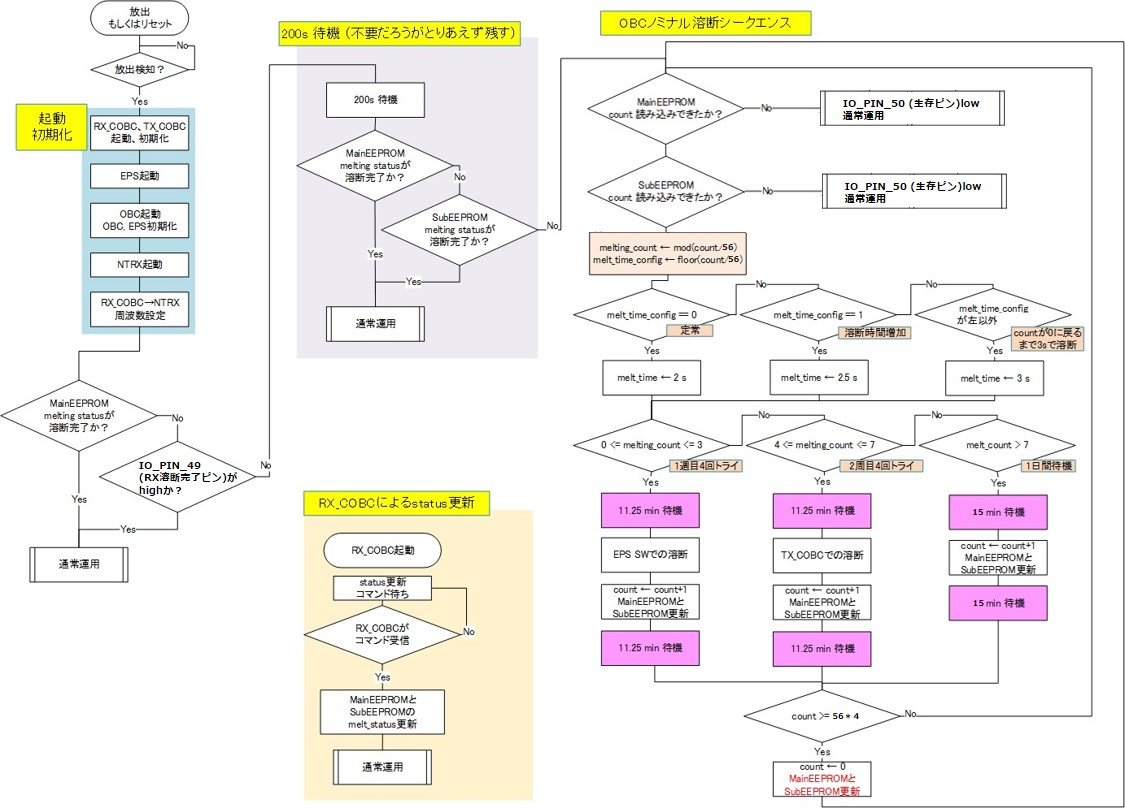
\includegraphics[scale=0.7]{03/fig/3-4-Ini-1.pdf}
	\caption{OBC正常時のフローチャート}
	\label{fig3-4-Ini-1}
\end{figure}	
\begin{itemize}
	\item OBCはRTOSを使い複数のタスクを持っているが起動時に動くのは初期運用のタスクのみである.
	OBCは起動後必ずOBC生存ピンである50番のIOピンをhighにする.
	\item EEPROMに書き込まれた溶断ステータスの計算式については1byteを1bitずつ加算その値が4以上だと溶断判断.これは放射線などの影響でbit反転の可能性を防ぐためである.
	\item countで溶断回数又は待機を判断しているが,これは待機途中にOBCの電源を落ちることを考慮し,定期的にEEPROMに書き込みを行う.
	\item OBCはEPSのWDTを管理しているので,初期運用時では初期運用のタスク内のループで叩きに行く構造(通常はOBCのコマンド確認で行っている詳細はOBCの章)
\end{itemize}
\subsubsection{OBC異常時初期運用モードソフト詳細(黒崎)}
OBC異常時のフローチャートを図\ref{fig3-4-Ini-2}に示す.
\begin{figure}[H]
	\centering
	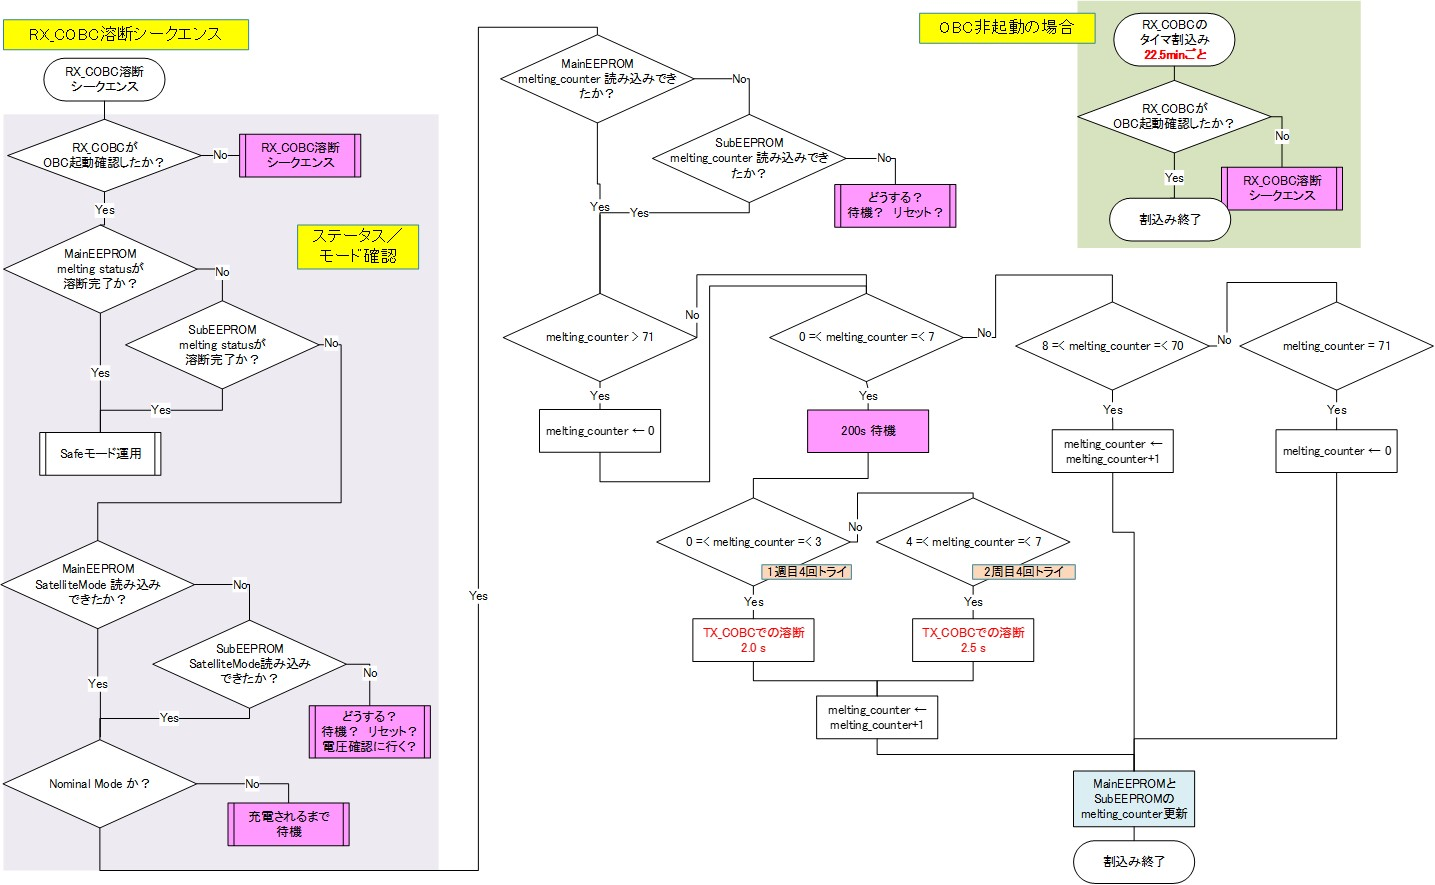
\includegraphics[scale=0.6]{03/fig/3-4-Ini-2.jpg}
	\caption{OBC異常時のフローチャート}
	\label{fig3-4-Ini-2}
\end{figure}	
\begin{itemize}
	\item RXPICで22.5分毎に行われるタイマー割込み処理内で,OBCの起動が確認できない場合,RXPICでの溶断シーケンスに入る.
	\item 溶断ステータス及び衛星モードを確認し,未溶断かつNominalモードの時に溶断処理に入る.
	\item EEPROMの溶断カウンターの値を読み込み,値に応じて溶断を行った後,溶断カウンターを更新する.
\end{itemize}

\subsubsection{初期運用 運用結果(黒崎)}
%以下のアクションの日付を書き足したいな...
アマチュア無線家からのCW HKデータ受信報告を受け,東工大地上局にて溶断停止コマンドをアップリンク.CW HKデータで溶断ステータスが溶断前から溶断済みに書き換わっていることを確認した.

\subsubsection{コメントや次回の改善点}
\hspace{2ex}
\textbf{OBC / CIB共通(黒崎・小出)}
\begin{itemize}
	\item 溶断済みフラグをCW HKデータのフリースペースの1byteに入れたのは神采配だったと思う.OrigamiSat-1の場合,アップリンクでEEPROMの指定アドレスを読んでダウンリンクする機能が使えなくなってしまっていたため,CW HKデータ以外に溶断済みを確認する術が無かった.
	\item OBCとCIBが同時に溶断を行ってしまった場合,バッテリーがどの程度減少するかの検証をできていなかった.
	\item OBCとCIBのどちらが,何回目の溶断で溶断を成功し,ダウンリンクを開始したかを分かるようにした方がいいのかもしれない.
	\item 「(3)開発の流れ」3-FにおけるOBC/CIBの統合は,初期運用のプログラムしか動かしていなかったので,モード切替やダウンリンクなども動かし,本番の運用を想定したデバックが必要であった.
	\item 溶断系統としてEPSのSWでの溶断,冗長系としてTXPICによる溶断があったが,EPSのSWにおける溶断はOBCのみしか使用できぬ仕組みになっていた.どちらでも溶断できるように
\end{itemize}

\hspace{2ex}
\textbf{OBC(小出)}
\begin{itemize}
	\item 初期運用を必ず成功させるために複雑なシークエンスにしてしまったが,もう少し簡潔なシークエンスのほうがよかったと思う.溶断時間の変化をなくして,プログラムを優しくする方法も考えられる.
\end{itemize}

\hspace{2ex}
\textbf{CIB(黒崎)}
\begin{itemize}
	\item FMに書き込んだプログラムでは,溶断ステータスは毎回,eepromを読み込んで判断としていたが,一度,溶断停止コマンドがアップリンクされて溶断ステータスが書き換わったら,PIC内のグローバル変数も書き換わるようなプログラムの方が良かったかもしれない.
	
	というのも,RXPICがeepromの読み込みができず,溶断ステータスを判断できない場合は全て「未溶断」判定にしていた.実際,OrigamiSat-1はeepromを読み込めないとい事象が起きてしまい,RXPICは毎回,初期運用モードに入り,200秒待機や溶断などをしてしまっていたと思われるため.
\end{itemize} %初期運用

\section{姿勢制御系}

\subsection{制御方式}
OrigamiSat-1 搭載の 5.8GHz 通信用パッチアンテナは指向性を持つため,同アン
テナ取付面を地上に向ける姿勢制御が必要となる.本衛星では,永久磁石と地
磁気の干渉を利用した受動的姿勢制御を採用した.飛行と姿勢のイメージを図
\ref{image_attitude_ctrl}に示す.衛星内部に搭載された棒磁石により姿勢
は地磁場の磁力線に沿う様に回転する.この過程で,日本の緯度付近を通過す
る際,パッチアンテナの面が地上を向く.但し,軌道上では運動を減衰させる
要素が乏しく,実際には磁力線を中心に揺動運動することとなる.このため,
本衛星では,PCパーマロイ製のヒステリシスダンパを搭載している.本ダンパ
は,磁力線の相対運動に伴い電磁誘導を生じ,内部抵抗による電力消費によっ
て,運動を熱に変換する.本方式は,同じく5.8GHzパッチアンテナを搭載して
いた,FITSAT-1(にわか)に採用され,実績があることから採用した.

\begin{figure}[htbp]
	\centering
	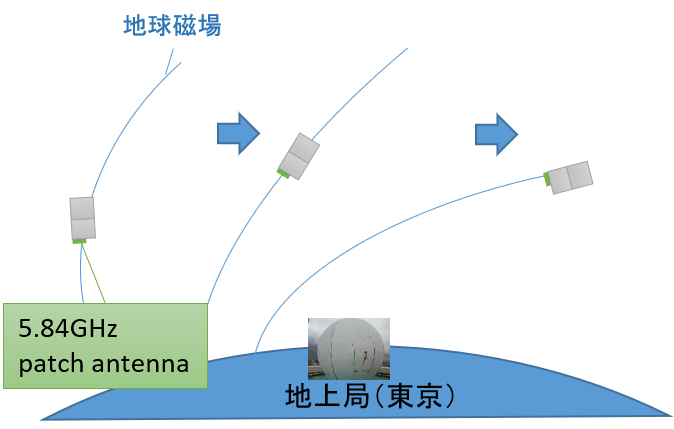
\includegraphics[width=10cm]{03/fig/image_attitude_ctrl.png}
	\caption{飛行と姿勢のイメージ}
	\label{image_attitude_ctrl}
\end{figure}

\subsection{主要諸元}
本衛星の姿勢制御用永久磁石およびヒステリシスダンパの搭載イメージを図
\ref{image_mag_HD}に示す.また,それぞれの諸元を表
\ref{spec_magnet}, 表\ref{spec_HD}に示す.

\begin{figure}[htbp]
	\centering
	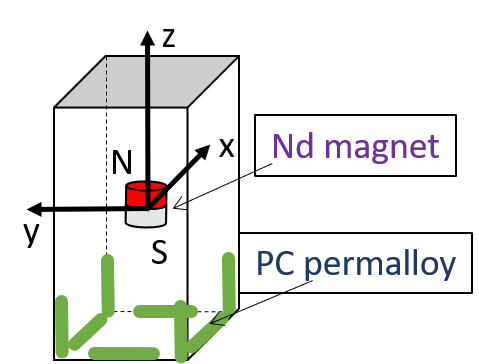
\includegraphics[width=5cm]{03/fig/image_mag_HD.png}
	\caption{永久磁石とヒステリシスダンパ搭載イメージ}
	\label{image_mag_HD}
\end{figure}

\begin{table}[htb]
    \centering
    \caption{OrigamiSat-1搭載磁石諸元}
    \begin{tabular}{cc} \hline
      項目 & 諸元 \\ \hline\hline
      材質 & Nd \\
        体積 & $2.73 \times 10^{-6} [\rm{m^3}]$\\ 
        磁束密度 & 0.468 [T] \\ 
        発生トルクオーダー & $10^{-5}$ [Nm] \\ \hline   
    \end{tabular}
    \label{requirment_op}
\end{table}

\begin{table}[htb]
    \centering
    \caption{OrigamiSat-1 搭載ヒステリシスダンパ諸元}
    \begin{tabular}{cc} \hline
      項目 & 諸元 \\ \hline\hline
        材質 & PC パーマロイ \\
        体積(X-axis) & 1.603 $\times 10^{-7} [\rm{m^3}]$ \\
        体積(Y-axis) & 1.320 $\times 10^{-7} [\rm{m^3}]$ \\
        体積(Z-axis) & 5.055 $\times 10^{-8} [\rm{m^3}]$ \\ 
        発生トルクオーダー & $10^{-6}$ [Nm] \\ \hline    
    \end{tabular}
    \label{requirment_op}
\end{table}




\section{構体系(奥山・大野) 重量管理も含む}

\if0
奥山
・工場の人と仲良くして納期短縮
・放出検知ピン(二硫化モリブデン,PEEK)
・基板保持ねじれ
・EMの不具合
・基板保持の治具
・精度出しの方法どうやって決めたか
・組立手順どう決めたか
・発注
・サーミスタ
・配線

ひらくさん
・組み立て精度が出せない(組み立てが異常に複雑)
・レールの長さが足りなかった →形状計測
・レールの粗さ計測を実施していなかった →形状計測
・ハードアノダイズ処理の2度手間が生じた(納期長い)
・FMでのディプロメントスイッチ不具合
・FM振動試験時、配線を噛んでしまっていた
  
  ----------------------------------------
  CAD作成
  ・干渉チェック
  ピッタリは危険(展開アンテナはまったやつ)
  ・EMの不具合:FM発注リスト参照
  ・CAD非反映物(ハーネス、コネクタ等)の考慮
  ・ハーネスの通り道にR
  ・ディプロイメントスイッチななめる
  ・工具が入るか パッチ土台とか
  
  図面作成
  ・加工時見やすいように
  ・公差の指定
  ・加工順序考える
  ・早めに工場と相談
  
  発注
  ・業者と工場の違い
  ・納期注意
  ・誰が見ても誤解しない図面
  ・アルマイト時間かかる マスキングとか
  
  
  加工
  ・ハードアノダイズ処理の2度手間が生じた(納期長い)
  ・基板保持ねじれ 組み立て?
  
  組み立て
  ・基板保持の治具
  ・基板入ったりはいらなかったり、、
  ・サーミスタ
  ・FM振動試験時、配線を噛んでしまっていた
  ・配線
  ・精度出しの方法どうやって決めたか
  ・組立手順どう決めたか
  ・組み立て精度が出せない(組み立てが異常に複雑)
  ・FMでのディプロメントスイッチ不具合
  ・手順書 誰でも組み立てられるように
  とくにバスはソフトの人もできるようにしておくべき
  全工程ソフトの人と確認
  ・工具は毎回しまう
  
\fi

本稿では,私が携わったEMの設計の修正からFMの組立までについて,各開発フェーズごとに記載する.
なお,詳細な不具合は「OP-S1-0065\_OrigamiSat-1不具合・A/I管理表\_20190124」に記載している.また,設計についてEMからFMで修正する際の修正項目(EMでの不具合項目)は「FM発注リスト.xlsx」に記載している.


\subsection{3DCAD設計}
3DCAD設計でミスが起こると開発が進んだときの出戻りが大きいので気をつける.
\subsubsection{干渉の確認}
構体の部品同士の干渉を確認する必要がある.ここで注意したいことが,加工公差である.CAD上では公差は指定していないため,公差を含めて干渉がないかを考慮する必要がある.EMでは,展開アンテナとそれを通す溝の幅が同じであったため,CAD上では干渉はないが,実際にはアンテナがはまって展開できなかった.(追加工で対応)
\subsubsection{ハーネス・コネクタ等の電子部品の考慮}
CADでハーネス,コネクタを入れることをお勧めする.ハーネスがどこを通るか,通る場所には通れるだけの隙間があるか,コネクタは干渉しないかを確認する必要がある.また,ハーネスは曲率の限界があるので注意する.
\subsubsection{ハーネスの通り道に突起物を置かない}
特に注意するのが,構造部品の角である.振動等でハーネスの皮膜が破れる恐れがあるため,Rをつける.また,さらに補強としてハーネスにガラスクロステープを巻いた.
\subsubsection{組立を考慮した設計}
組み立てについては,工具の大きさと,組み立てのしやすさを考慮する必要がある.工具の大きさについては,組み立て時に工具と部品に干渉なく組み立てられるかを注意する.底面パネルに対するパッチアンテナ土台の取り付けは,取り付けるねじに対して工具を同軸で取り付けるべきであるが,底面パネルと工具が干渉するので,工具を斜めにして取り付けていた.組み立てのしやすさについては,D-subの取り付け等無理な体勢での組み立てがあったので,良くない.何度かワッシャを構体内に落としたこともあったので注意して欲しい.
\subsubsection{ばか穴による組み立てのズレの考慮}
ばか穴にしている箇所は,ねじの径との差の範囲で部品間が相対的にずれる.0.1mmオーダーの差があり,レール精度は±0.1mmであるので,十分影響がある.要求精度以外にも,ディプロイメントスイッチの接触不良があった.スイッチの位置によってディプロイメントピンとの相対的位置関係が変わり,スイッチ起動の要求,インターフェイスを満たせない場合があった.今回はスイッチ取り付け後のピンを取り付ける際に位置を調整することで対処した.


\subsection{図面作成}
図面作成は寸法を全て書き込めば良いだけでなく,加工する際に必要な寸法を書くことが重要である.自ら加工することも少なくなかったので,そのような経験があるとよりうまく書けると思う.
%%\subsubsection{加工者への考慮}

%%\subsubsection{公差の指定}
\subsubsection{加工順序の考慮}
自分で加工するとき,前日までに加工順序を確認しておくことをお勧めする.当日朝から工場に行ってから工程を考えると進捗が得られない.
\subsubsection{加工者との早めの相談}
公差等わからないことがあったら専門家に聞くほうが良い.考えるより細かい部分は話しながら決めたほうが早く進む.


\subsection{発注}
発注は相手に誤解されないように伝えることが重要である.
\subsubsection{業者と工場の違い}
基本的には工場の発注が良い.工場のメリットは大学内に併設しているので直接コンタクトがとりやすい.外部業者であるとメールのみのやり取りで伝えきれないことがあったりする.外部業者は,工場が立て込んでいて納期が遅かったり,休業のときに利用する.工場は大学内の様々な案件を行っているので,時期によっては納期がだいぶ先になる.また,外部業者で工場が海外であると日本と休日が異なるため,助かることがある.(特にGW)
%%\subsubsection{納期の考慮}


\subsection{組み立て}

\subsubsection{手順の決め方}
基本的には底面パネルから膜展開部に向かって組み立てる.それに加え,左記の流れであると組めない部分は順序を適宜変えた.また,レール精度が求められている部品(底面パネル,側面パネル×4,膜展開部)に関してはトルクはかけずに仮締めを行い,その後精度出しを行った.最終的な手順は「組み立て手順書」に記載する.
\subsubsection{手順書の作り方}
誰でも組み立てができることを目標とした.組み立て時に考えることはないようにする.また,ソフトを書く人にはバス系の組立ができるようにしてもらうことを薦める.ソフトを書き込むために分解が必要なときもあるので,そのたびに構体系の担当がいないと開発が進まない事態になったことが何度もあった.
\subsubsection{精度出しの方法}
精度出しの方法は「組み立て手順書」に記載している.
\subsubsection{基板保持の冶具}
基板保持とCIBの取り付け誤差により,基板がずれて側面パネルが固定できないことが何度かあった.それにより,基板保持とCIBの相対位置を固定する冶具を作成した.
\subsubsection{基板の組み立て誤差}
上記の対応で精度は良くなったが,その先の基板を取り付けた際に再現性がなく,側面パネルと干渉することがあった.これの原因はわかっていない.
\subsubsection{サーミスタの貼付方法}
サーミスタを貼り付ける際は貼り付ける部品にカプトンテープを貼り,その上にサーミスタを置き,上からカプトンテープを貼る.このとき,どちらのカプトンテープも多数の穴を開けた.これは,真空中でカプトンと部品との間の気泡が膨張し,カプトンがはがれることを防ぐためである.
\subsubsection{配線}
ハーネスの経路は,構体部品との干渉を避けることとハーネスの可動域を考慮してどのように動いても 部品間でハーネスをはさまないよう取り回すことを考慮する.後者についてはFMの1回目の振動試験でハーネスを構体部品ではさんでしまっていたので,はさんでしまったハーネスを別のハーネスをくぐらせて動いたとしても挟まれないようにした.
\subsubsection{ディプロイメントスイッチの不具合}
ディプロイメントピンの公差の指定を誤り,底面パネルにピンが固着してしまった.対策としては,底面パネルの穴を削り,微調整した.また,ピンには二硫化モリブデン処理を施し,摩擦係数を減らした.
\subsubsection{工具の管理}
工具は作業が終わっていなくてもその日中には片付けることを徹底する.放置したり,他の人が使ったりした後,翌日に探すことが多々あった.構体系のみならず開発者全員の認識が必要である.



\section{熱系(中村・坂本)}

\subsection{熱設計の方針}
熱系については,下記の考え方のもと設計・検証を実施した.この考え方は主に,戸谷剛・北海道大学准教授がふくい宇宙産業創出研究会WGで講演(2016年11月24日)された資料をご厚意で見せていただき,そこからの学びを元に構築した.
\begin{itemize}
	\item 温度が均一化できるところをなるべく増やし,複雑度を下げる方針とした.
	\item Thermal Desktop等解析ソフトを用いた詳細解析は行わず,解析については少数節点解析でのパラメータサーベイのみを行った.結果,当初設計の表面仕上げで良いとの見込みのもと開発を進めた.
	\item 受動的熱制御を主体とした.ただし,開発の最後のフェーズでバッテリにヒータを貼付し,能動的熱制御を取り入れる設計変更をした.
	\item 材料の熱光学パラメータは宇宙科学研究所小川研のご厚意で,TESA2000を使用させていただき計測した.
	\item 接触コンダクタンスの影響を少なくするため熱伝導シートを導入した.
	\item ウェルリサーチ社の熱真空槽を用い,熱平衡試験でパラメータ同定をしたのちに,熱真空試験で機器の動作確認をした.これらの試験については別章に記載する.
\end{itemize}

下図のように節点へ分割したモデルを作成した.Matlabを用いin-houseでプログラムを書いた.
\begin{figure}[H]
	\centering
	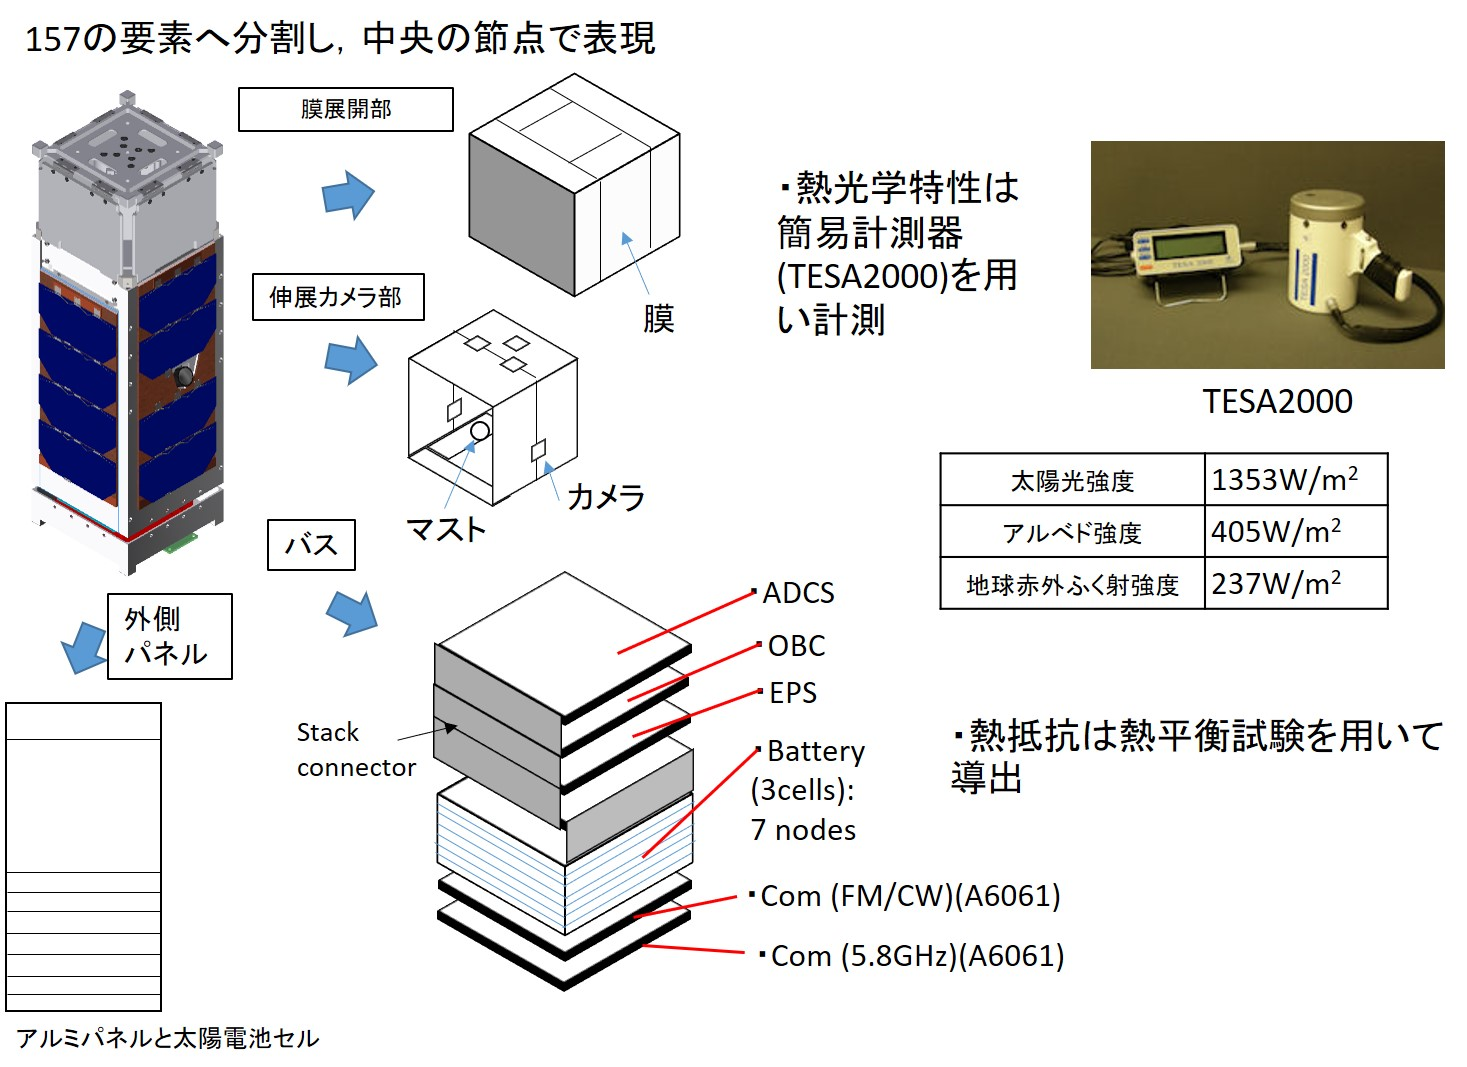
\includegraphics[width=0.8\textwidth]{03/fig/3-7-1.jpg}
	\caption{節点法による熱解析}
	\label{fig3-7-1}
\end{figure}

パラメータ同定のために熱平衡試験を実施した.試験については別章にて詳説する.概要を数に示す.
\begin{figure}[H]
	\centering
	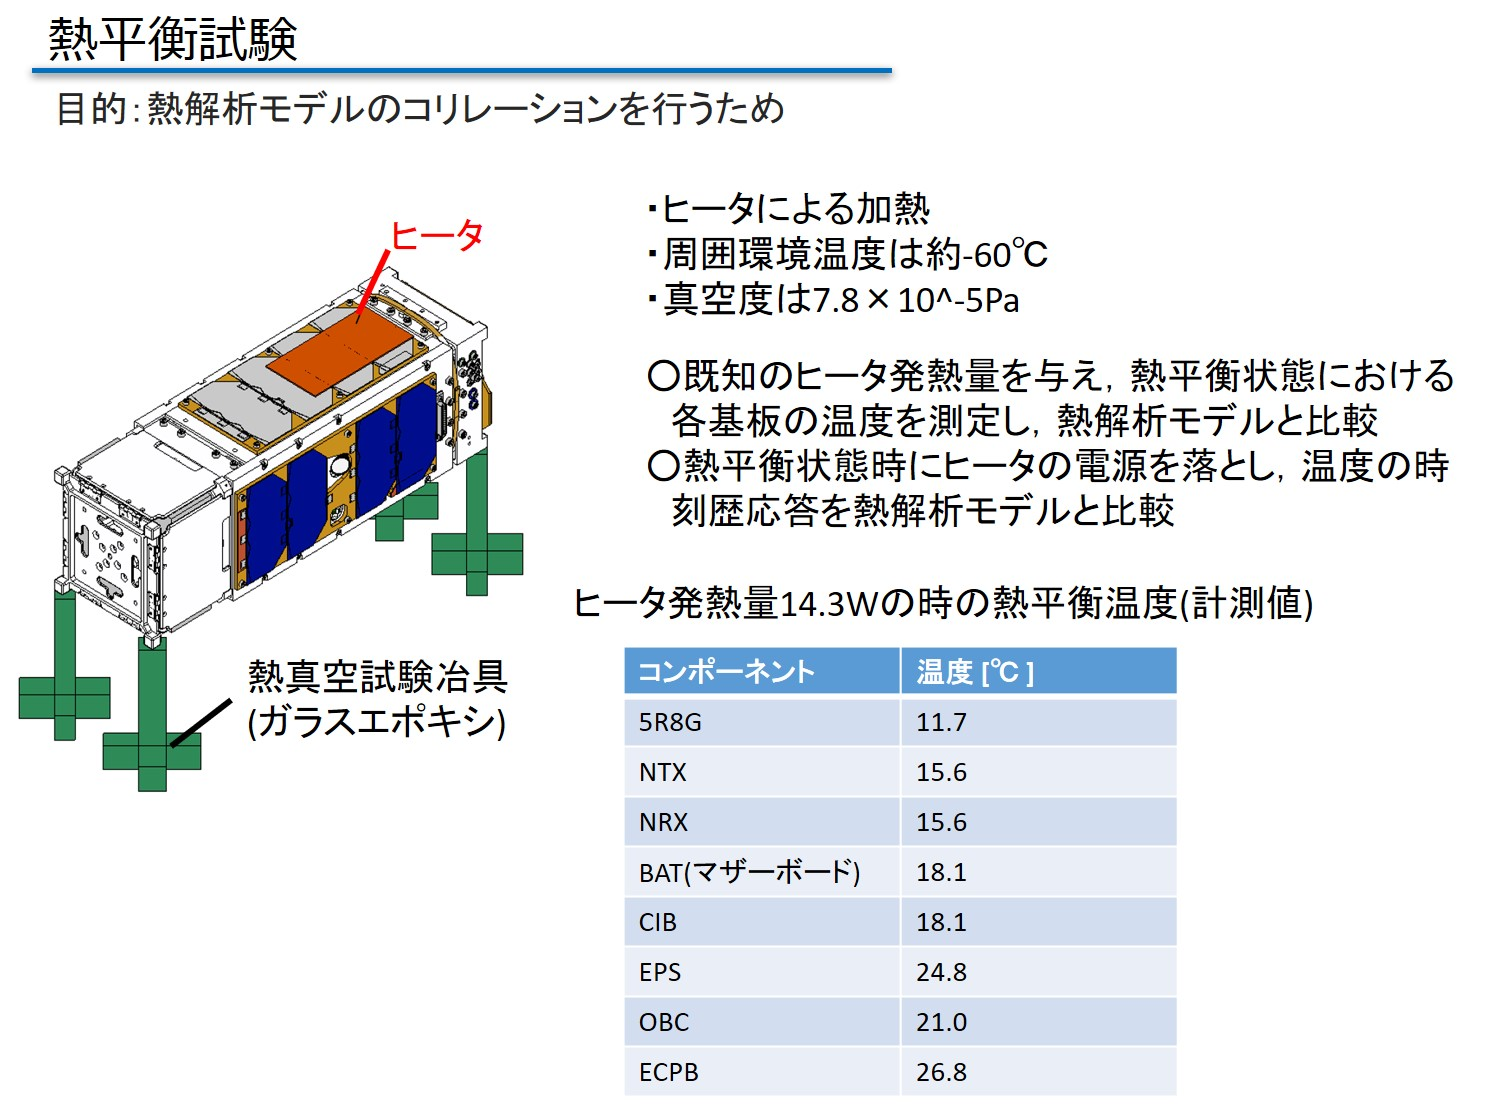
\includegraphics[width=0.8\textwidth]{03/fig/3-7-2.jpg}
	\caption{熱平衡試験による解析モデルコリレーション}
	\label{fig3-7-2}
\end{figure}
ここで得たパラメータを元に,節点解析モデルを用いて,軌道上での各節点の温度変化を予測した.

\subsection{熱解析結果:高温ケース}
高温ケースで以下の結果を得た.
\begin{figure}[H]
	\centering
	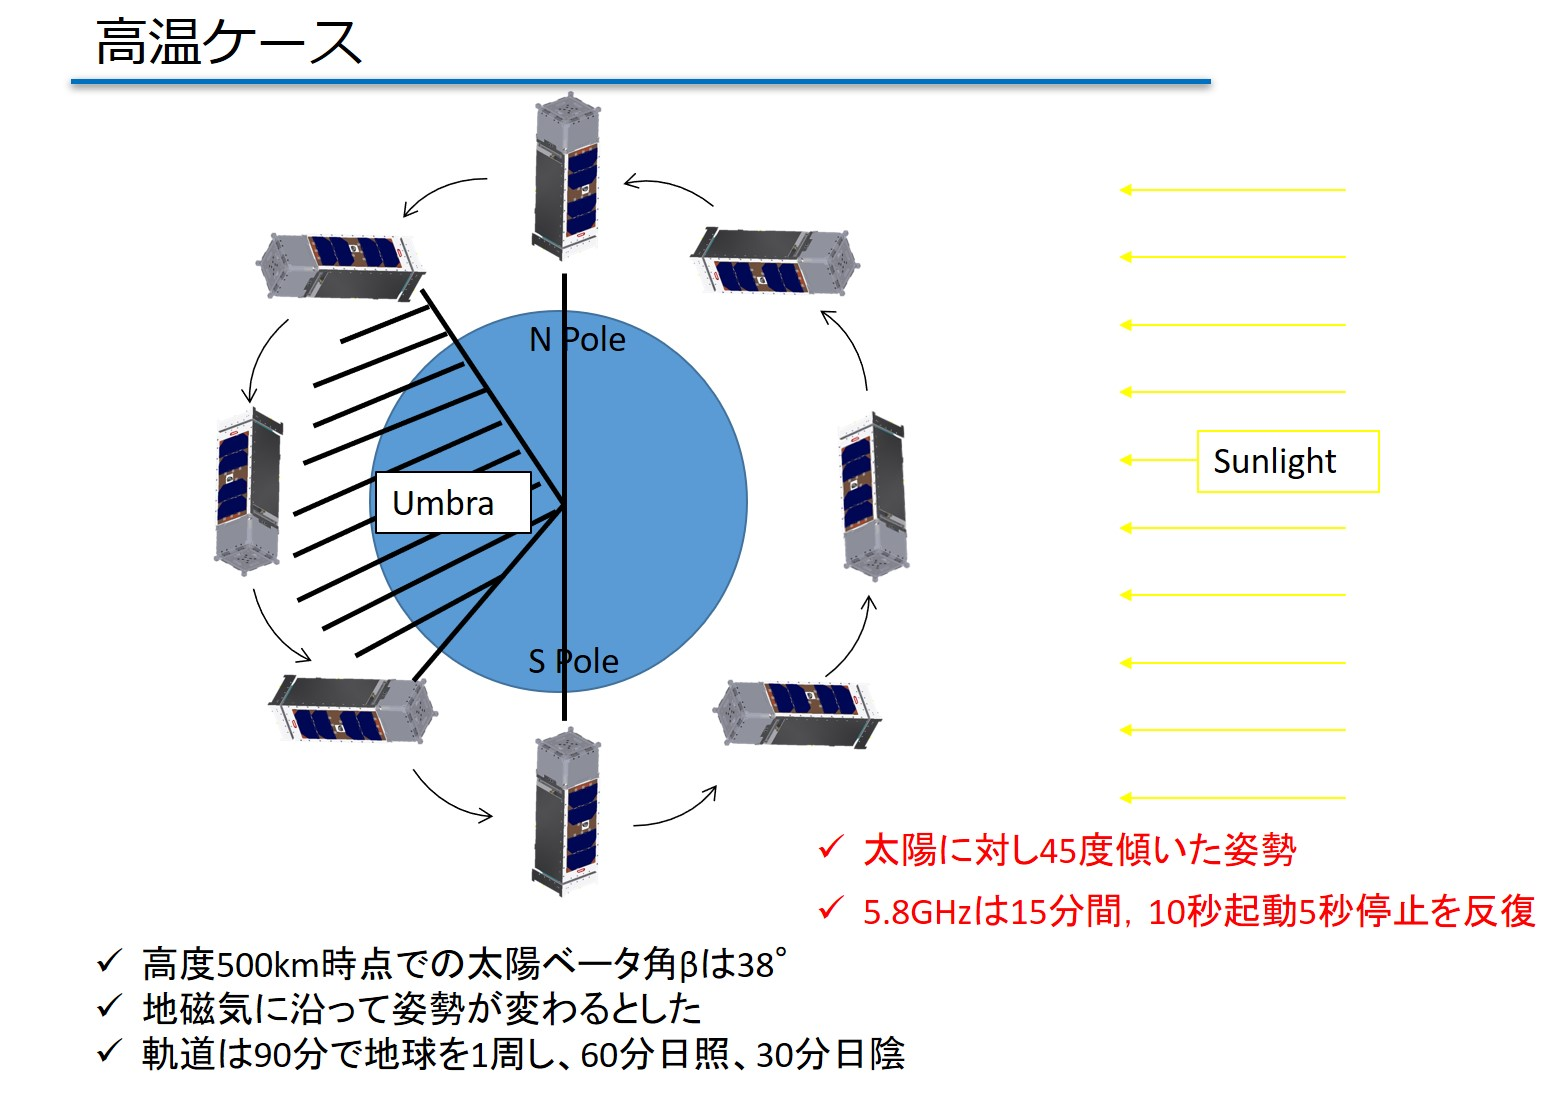
\includegraphics[width=0.5\textwidth]{03/fig/3-7-3.jpg}
		\includegraphics[width=0.5\textwidth]{03/fig/3-7-4.jpg}
				\includegraphics[width=0.5\textwidth]{03/fig/3-7-5.jpg}
	\caption{節点法熱解析結果:高温ケース}
	\label{fig3-7-3}
\end{figure}

\subsection{熱解析結果:低温ケース(Nominal)}
膜展開前の低温ケースで以下の結果を得た.
\begin{figure}[H]
	\centering
	\includegraphics[width=0.8\textwidth]{03/fig/3-7-6.jpg}
	\includegraphics[width=0.8\textwidth]{03/fig/3-7-7.jpg}
	\caption{節点法熱解析結果:低温ケース(Nominal)}
	\label{fig3-7-6}
\end{figure}

\subsection{熱解析結果:低温ケース(膜展開後)}
膜展開後の低温ケースで以下の結果を得た.
\begin{figure}[H]
	\centering
	\includegraphics[width=0.8\textwidth]{03/fig/3-7-8.jpg}
	\includegraphics[width=0.8\textwidth]{03/fig/3-7-9.jpg}
	\caption{節点法熱解析結果:低温ケース(膜展開後)}
	\label{fig3-7-8}
\end{figure}

\subsection{熱系の振り返り}
別章に掲載する軌道上温度のHKデータを見ると,解析結果よりも温度が高く,また温度変化の幅も小さい.したがって解析・実験による予測が適切でなかった可能性がある.
軌道上結果を見る限りでは,バッテリにヒータを追加する設計変更は不要だった可能性がある(ただし膜を展開していないので膜展開時についてはさらなる詳細解析を要する).

\section{VHF/UHF展開アンテナ(仁尾・坂本)}



\section{ミッション系}
\subsection{5.8GHz通信ミッション(井手)}
ここでは5.8GHz通信モジュール(以下5.8)について記述する
\subsection{伸展カメラ}
\subsubsection{システム開発(ウェル・坂本)}



\subsubsection{3次元計測(飯島・黒崎)}



\subsubsection{動画計測(飯島・坂本)}

ラズベリーパイのカメラを用いての膜展開の動画撮影を実現するため,以下のように実験を実施しながら設計の改良とその検証を行った.\\
\\

\noindent \textbf{2016/05/26 三脚上に設置した伸展カメラ部BBMによる膜展開撮影}
\begin{itemize}
	\item 古谷研にて実施.参加者:古谷,坂本,下田(ウェルリサーチ),仲鉢,天本,中村.
	\item 航空機実験用の膜(70cm×70cm)の展開を,三脚上に設置したラズパイカメラで撮影.
	\item 部屋の蛍光灯をOFFして撮影したが,窓を暗幕で覆っていないため照度が高かった(LED点灯なしでも130ルクス程度).
	\item 80fpsで320X240ピクセルで撮影.問題なく撮影できた.
	\item 課題: 撮影範囲が狭い.広角レンズの使用,および撮影スピードを半分に下げる検討.
\end{itemize}
\begin{figure}[H]
	\centering
	\includegraphics[width=.9\textwidth]{03/fig/3-9-2-3-1.jpg}
	\caption{三脚上に設置した伸展カメラ部BBMによる膜展開撮影の実験構成}
	\label{fig3-9-2-3-1}
\end{figure}
\begin{figure}[H]
	\centering
	\begin{tabular}{cc}
		\begin{minipage}{0.5\hsize}
			\begin{center}
				\includegraphics[width=1\textwidth]{03/fig/3-9-2-3-2.jpg}
			\end{center}
		\end{minipage}&
		\begin{minipage}{0.5\hsize}
			\begin{center}
				\includegraphics[width=1\textwidth]{03/fig/3-9-2-3-3.jpg}
			\end{center}
		\end{minipage}\\
		\begin{minipage}{0.5\hsize}
			\begin{center}
				\includegraphics[width=1\textwidth]{03/fig/3-9-2-3-4.jpg}
			\end{center}
		\end{minipage}&
		\begin{minipage}{0.5\hsize}
			\begin{center}
				\includegraphics[width=1\textwidth]{03/fig/3-9-2-3-5.jpg}
			\end{center}
		\end{minipage}
	\end{tabular}
	\caption{三脚上に設置した伸展カメラ部BBMによる膜展開撮影結果}
	\label{fig3-9-2-3-2}
\end{figure}

\noindent \textbf{2017/04/18 伸展マスト付き織物膜(EM1)展開撮影実験}
\begin{itemize}
	\item 古谷研にて実施.参加者:東工大古谷研、坂本研、首都大鳥阪、西井、ISAS名取、奥泉、佐藤(敬称略).実験の詳細は膜展開部の項で述べる.
	\item 膜上のデバイスもダミーを設置した(ただしハーネスはなし).1mブームの上部に伸展カメラ部BBMを天井から吊り下げて設置した.伸展カメラ部に伸びるハーネスもダミーを取り付けた.広角レンズを使用.
	\item 部屋の蛍光灯をONした状態で展開.40fpsに落として,撮影画角を広くしたところ,全体の展開動画が撮影できた.
	\item 課題: 照明条件と反射マーカーを模擬した上で,暗闇の中での撮影可能性を検証する必要がある.→この実験後,SDDL暗室内でLED+マーカーを動画撮影し,撮影できる見込みを得てEM製作を実施した.
\end{itemize}
\begin{figure}[H]
	\centering
	\includegraphics[width=.8\textwidth]{03/fig/3-9-2-3-6.jpg}
	\caption{伸展マスト付き織物膜(EM1)展開撮影結果}
	\label{fig3-9-2-3-6}
\end{figure}

\noindent \textbf{2018/04/23 暗室での織物膜(EM2)動画撮影試験}
\begin{itemize}
	\item 古谷研にて実施.窓を暗幕でふさぎ,照明をOFFして暗闇の中で実験した.床からの照り返しを避けるため,床にも暗幕を敷いた.
	\item FMとほぼ同じ仕様でマーカーを貼り付けたEM2膜の展開時,および展張後に,膜から高さ1mに吊り下げた伸展カメラ部BBMからのLEDの照明のみで動画撮影を行った.
	\item 綺麗に展開の動画が撮影できた.ただ照明がやや強すぎる(マーカーが光りすぎている)と考え,開いた後の膜を手で揺らしながら,LEDの明るさを徐々に暗くして適切な明るさへ調整した.
\end{itemize}
\begin{figure}[H]
	\centering
	\includegraphics[width=.8\textwidth]{03/fig/3-9-2-3-7.jpg}
	\caption{伸展カメラ部LED照明織物膜(EM2)展開撮影結果}
	\label{fig3-9-2-3-7}
\end{figure}
\subsection{膜展開部}
\subsubsection{展開膜開発(古谷・坂本)}





\subsubsection{MDC(大本)}

\begin{itemize}
	\item 基本設計思想\par
	MDC(Membrane Device Contoroller)は膜上に取り付けられたSMAアンテナの利得計測,ひずみ値計測,薄膜太陽電池のIV特性計測,膜の温度計測,伸展マスト先端のIMU情報の計測,膜展開を行うテグス溶断の冗長系を担うことを目的として新規開発を行った基板であり,伸展マスト先端の膜上デバイス制御部に取り付けられている.
	
	
	\item プログラム概要\par
	プログラムの機能としては以下の3つがある.
	\begin{enumerate}
		\item OBCからのコマンドに従い,各データを取得し,EEPROMに保存
		\item OBCからのコマンドに従い,指定されたEEPROMのアドレスから指定されたデータ数をOBCに送信
		\item OBCからのコマンドに従い,膜展開を行うテグスを溶断
	\end{enumerate}
	この中で,SMAアンテナの利得,ひずみ値計測は開発の遅れから断念した.
	
	\item コメントや次回への改善点\par
	MDC開発はバス部開発の遅れからあまり力を入れることができず,SMAアンテナミッションを諦めたり,その他の機能についても最低限の機能しか搭載することができなかった.
	
\end{itemize}



\subsubsection{薄膜太陽電池ミッション(大野)}






\subsubsection{SMAアンテナミッション(鳥阪・坂本)}

東京都立大学の鳥阪がこのアドバンストミッションを主導した.宇宙科学研究所の川崎研究室にご支援をいただいた.(このつながりもあって,5.8GHz通信ミッションの検証の目的で川崎研究室の電波暗室を使用させていただいた.)

膜上において,SMAアンテナによるOrigamiSat-1のCW受信と,ひずみゲージを用いた形状計測を目指した.しかし最初にミッションを遂行できる基板がシステム側にもたらされたのがFM膜の最後の収納時であったため,バス部との電気統合を行わないままに膜上に貼付した.膜収納後,FMのMDC基板との電気統合を試みた.しかし,膜上のSMAアンテナ基板と,バス部のMDC基板間で通信ができなかった.この不具合対応をしている時間はなかったため,SMAアンテナからのハーネスを,MDC基板へ結合しなかった.目指したSMAアンテナミッションについて,鳥阪が筆頭著者となり下記ジャーナル論文を出版した.

\noindent A.~Torisaka, et al., ``Development of shape monitoring system using SMA dipole antenna on a deployable membrane structure,'' Acta Astronautica, Vol.~160, July 2019, pp.~147--154.

少なくとも,膜上にSMAアンテナと剛なアンテナ基板を搭載した状態で,膜面の収納・展開を確認できた.この達成により,革新3号機HELIOSの膜上アンテナミッションおよび干渉計ミッションの提案につながった.




\subsubsection{球状太陽電池ミッション(サカセ・坂本)}

サカセアドテック社の主導により,スフェラーパワー社(京都府)が開発した球状太陽電池「スフェラー」と三軸織物を組み合わせた球状太陽電池デバイスを開発し,膜上に搭載した.
球状太陽電池の発電により,三軸織物上に搭載されたLEDが光る.このLED光を,伸展カメラ部の写真撮影により確認することを目指した.
伸展カメラ部の写真撮影は,地球の影で実施するため,暗闇でも球状太陽電池が発電するように,膜上デバイス制御部の側面に2つの赤外線LEDを取り付け,この赤外線LEDを光で球状太陽電池が発電し膜上でLEDが光る,という設計とした.
球状太陽電池について詳細には,膜展開部と同じく,文部科学省に提出した報告書に詳しく記載している.

表,裏のどちらの面から光が照射しても発電が可能な宇宙用デバイスの提案を目指し,フライトモデルへの実装を達成した.デバイスを貼付した膜がコンパクトに収納できること,そして地上試験で展開もできることを確認できた.







	% 3章 サブシステム開発の経緯(設計・試験)
% 4章
\chapter{統合試験}
\label{chap:test}

%********************************
%図の追加
%\begin{figure}[H]
%	\centering
%	\includegraphics[scale=1]{04/fig/4-2-1.jpg}
%	\caption{図の説明文}
%	\label{fig4-2-1}
%\end{figure}
%
%%表の追加
%\begin{table}[H]
%	\centering
%	\includegraphics[scale=1]{04/fig/t4-2-1.jpg}
%	\caption{表の説明}
%	\label{table4-2-1}
%\end{table}
%********************************

\section{放射線試験(寺田(報告書)・池谷・黒崎)}
\subsection*{関連文書}
\begin{itemize}
	\item OP-S1-0126 球状太陽電池放射線試験結果
\end{itemize}
\subsection{試験概要}
\subsubsection{目的}
本試験では,多量の放射線が入射することに起因する電離効果のうち,トータルイオンドーズ効果が機器に与える恒久的損傷を調べた.これにより,新規開発基盤である通信\&インヒビット基板(CIB)および膜上デバイス制御(MDC)基板に関して,ミッション期間中に受ける損傷具合を試験した.

シングルイベント(Single Event Effects=SEE)試験はプロジェクトの進行状況および人員を考慮し行われなかったものの,本来は実施されるべきである.


表\ref{table_4_date}に全5回の試験日時,$\gamma$線照射時間をまとめた.
\begin{table}[htbp]
	\centering
	\caption{放射線試験 試験日時一覧}
	\label{table_4_date}
	\begin{tabular}{ccccc}
		\hline\hline
		回& 日付 & 開始 & 終了 & 最大照射時間[h]  \\ \hline
		1&2017/2/6 &11:00  &17:30&6.0  \\
		2&2017/7/13  &14:00  &18:00&3.0  \\
		3&2017/7/26  &11:00  &17:30&3.0  \\
		4&2018/2/9  &11:00  &16:30&3.0 \\
		5&2018/5/28  &14:00  &18:00&3.0 \\\hline\hline
	\end{tabular}
\end{table}

最初の放射線試験はBBM開発段階において,CIBやMDCの開発も進んでいない中,膜面搭載の球状太陽電池および膜面制御部に設置される赤外線LEDに関して,ミッション期間中に受ける損傷具合を試験した.続く第二回以降の試験ではCIB,MDC搭載のICを中心に試験が行われ,照射中にデータロガーを用いた電圧,電流,温度の計測が行われた.第三回以降ではさらにPCと通信させることにより,データ伝送が正常に行われるか確認した.第四回試験ではEM開発中に増えたIC並びに,照射量が不十分であったICの試験を行った.第四回で通信用のマイコンに不具合発生が確認されたた,最後に追試験(第五回)を行い搭載するマイコンを変更した.

\vspace{3ex} 
\textbf{コメント}
\begin{itemize}
\item 実験室を予約する場合は,照射時間だけでなく,前後の準備撤収時間を考慮し最低1時間は余分に予約する.
\item 第5回試験では1名のみで当日,準備から実験まで行ったが,照射室とPC等を置く場所は離れているので,2名いた方が準備しやすいと思う.
\item 上記コメントに追記:照射中は最大二人,セットアップと撤収には最低二人必要であると考える.
\end{itemize}
	
\subsubsection{試験場所}
東京工業大学 大岡山キャンパス 大岡山北実験棟1 コバルト60照射室

\vspace{3ex} 
\textbf{コメント}
\begin{itemize}
	\item 予約はメールでやり取りを行う.
\end{itemize}


\subsection{試験供試体および照射条件}

供試体一覧を表\ref{tab:tidic}に示す.


\begin{landscape}
\begin{table}[htbp]
	\centering
	\caption{放射線試験 試験供試体,照射量,試験条件,および確認項目}
	\label{tab:tidic}
	
	%\scalebox{0.9}{
	\scriptsize
	\begin{tabular}{c|c|c|c|c|c|c|c|l|l}
		\hline\hline
		回                   &                      & 型番                   & 搭載箇所                 & 線量       & 照射時間         & 距離           & データロガー計測項目           & その他確認項目                 & 備考                    \\
		                   &                      &                  &                 & {[}Gy{]}        &  {[}h{]}         & {[}cm{]}          &           &                &                  \\ \hline
		1   & 球状太陽電池               &                      & 膜                    & 14883                & 6                    & 10                   &                      & 点灯確認                 &                       \\
		& 赤外線LED               & OSI5LA5113A          & 膜展開部                 & 14883                & 6                    & 10                   &                      & 点灯確認                 &                       \\\hline
		2   & DCDCコンバータ            & TPS55330             & CIB                  & 39                   & 0.5                  & 60                   & 出力電圧,入力電流,温度         &         &                       \\
		& リニアレギュレータ            & TA78033AF         & CIB                  & 39                   & 0.5                  & 60                   & 出力電圧,入力電流,温度         &         &                       \\
		& ダイオード                & B540-13-F            & CIB                  & 39                   & 0.5                  & 60                   &                      & 逆電流が流れないか            &                       \\
		& オペアンプ                & AD8657ARM            & MDC                  & 39                   & 0.5                  & 60                   & 温度                   & 照射前後の機能確認         &                       \\\hline
		3  & マイコン                 & PIC16F887            & CIB                  & 231                  & 3                    & 60                   & 入力電流                 &                      &                       \\
		& マイコン                 & PIC18F25K80          & MDC                  & 231                  & 3                    & 60                   & 入力電流                 &                      &                       \\
		& CANトランシーバ            & MAX3051ESA+          & MDC                  & 231                  & 3                    & 60                   & 入力電流                 & mbedにより信号確認          & 80分(103 Gy分)後動作不良 \\
		& シャントレギュレータ           & TL431                & MDC                  & 231                  & 3                    & 60                   & 出力電圧,入力電流,温度         & 出力電圧,入力電流,温度         &                       \\
		& 加速度センサ               & ADXL345              & CIB                  & 231                  & 3                    & 60                   & 入力電流                 &                      &                       \\
		& ジャイロセンサ              & ITG-3200             & CIB                  & 231                  & 3                    & 60                   & 入力電流                 &                      &                       \\
		& 対数検出器                & ADL5513ACPZ          & 膜上アンテナ               & 16830                & 3                    & 0                    & 出力電圧,入力電流            &                      &                       \\\hline
		4  & マイコン                 & PIC16F887            & CIB                  & 213                  & 3                    & 60                   &                      & mbedにより信号確認          & 60分(71 Gy分)後動作不良  \\
		& マイコン                 & PIC16F886            & CIB                  & 213                  & 3                    & 60                   &                      & mbedにより信号確認          &                       \\
		& DCDCコンバータ            & TPS55330             & CIB                  & 213                  & 3                    & 60                   & 出力電圧                 &                      &                       \\
		& モデム                  & FX614                & CIB                  & 213                  & 3                    & 60                   &                      & mbedにより信号確認          &                       \\
		& ADコンバータ              & MAX11605             & CIB                  & 213                  & 3                    & 60                   &                      & mbedにより信号確認          &                       \\
		& ダイオード                & B540-13-F            & CIB                  & 213                  & 3                    & 60                   &                      & mbedにより電圧確認          &                       \\
		& レギュレータ               & TA78033AF            & CIB                  & 213                  & 3                    & 60                   &                      & mbedにより電圧確認          &                       \\
		& MOSFET               & SK8603140L           &                      & 213                  & 3                    & 60                   & 出力電圧                 &                      & 搭載されず                 \\
		& ダイオード                & RB080L-30            & CIB                  & 213                  & 3                    & 60                   &                      & mbedにより電圧確認          &                       \\
		& PhotoMOS             & AQY211G2S            & CIB                  & 213                  & 3                    & 60                   & 出力電圧                 &                      &                       \\
		& PhotoMOS             & AQV252G3S            & CIB, MDC             & 213                  & 3                    & 60                   & 出力電圧                 &                      &                       \\
		& タイマー                 & SA555                &                      & 213                  & 3                    & 60                   & 出力電圧                 &                      &                       \\
		& マルチプレクサ              & ADG821BRMZ           &                      & 213                  & 3                    & 60                   & 出力電圧                 &                      &                       \\
		& レギュレータ               & TA7805AF             &                      & 213                  & 3                    & 60                   &                      & mbedにより電圧確認          & 搭載されず                 \\
		& MOSFET               & MTM232230LBF         &                      & 213                  & 3                    & 60                   & 出力電圧                 &                      &                       \\
		& マイコン                 & PIC18F25K80          & MDC                  & 71                   & 1                    & 60                   &                      & 照射前後の機能確認            &                       \\
		& CANトランシーバ            & MAX3051ESA+          & MDC                  & 71                   & 1                    & 60                   &                      & mbedにより信号確認          &                       \\
		& 加速度センサ               & ADXL345              & MDC                  & 71                   & 1                    & 60                   &                      & 照射前後の機能確認             &                       \\\hline
		5   & マイコン                 & PIC16F887            & CIB                  & 80                   & 3                    & 100                  &                      & mbedにより信号確認          &                       \\
		& マイコン                 & PIC16F886            & CIB                  & 80                   & 3                    & 100                  &                      & mbedにより信号確認          &                       \\
		& マイコン                 & PIC16F887            & CIB                  & 80                   & 3                    & 100                  &                      & mbedにより信号確認          &                       \\
		& WDT                  & SA555                & CIB                  & 80                   & 3                    & 100                  & 出力電圧                 &                      &  \\ \hline\hline
	\end{tabular}
\end{table}
\end{landscape}

図\ref{fig4-1-2}並びに,図\ref{fig4-1-4}はそれぞれ第四回,五回の供試体である.

\begin{figure}[htbp]
	\centering
	\includegraphics[scale=0.9]{04/fig/4-1-2.jpg}
	\caption{第四回試験供試体拡大図}
	\label{fig4-1-2}
\end{figure}

\begin{figure}[htbp]
	\centering
	\includegraphics[width=70mm]{04/fig/4-1-4.jpg}
	\caption{第五回試験供試体拡大図}
	\label{fig4-1-4}
\end{figure}


\vspace{2ex} 
\textbf{コメント}
\begin{itemize}
	\item 第五回試験を第四回と異なる試験条件(線源までの距離,照射時間)で試験を行ったが,第四回と試験条件を揃えるべきだったかもしれない.
\end{itemize}



\subsection{照射量}
OrigamiSat-1のCIB周り,およびMDC基板周りのアルミニウム構体板厚は2 mmである.NASA SSP 30512 Revision C によると高度500km,軌道系射角 $51.6 ^{\circ}$の環境において厚さ2.032 mmのアルミニウムに囲まれている場合の1年あたりトータルドーズ量 1.012E+03 rad(10.12 Gy)である.使用期間をCI基板は1年,MDC基板は4か月とした場合の被ばく量はそれぞれ約10.12 Gy,3.73 Gyとなる.第四回試験においては,両基板ともに両面にICが搭載されているため0.5 hごとに基板の表裏をひっくり返した.線源に対して裏面にあるICの被ばく量は表面にあるICの被ばく量に対して微小であると仮定した.

参考としてコバルト60照射室の線量率と線源からの距離の関係を表\ref{tab:tidrate}にまとめた.
さらに線源から60 cm,100 cmの距離に置かれた実験の様子を図\ref{fig4-1-1},図\ref{fig4-1-3}に示す.

\begin{table}[htbp]
	\centering
	\caption{コバルト60照射室 線量率}
	\label{tab:tidrate}
	
	\begin{tabular}{c|cccc}
		\hline\hline
		距離(cm)   & 0        & 10       & 60       & 100      \\
		単位(Gy/h) & $\times10^3$     & $\times10^3$     & $\times10^2$        & $\times10$      \\ \hline
		2017.2   & 5.926781 & 2.590717 & 0.814838 & 3.147849 \\
		2017.7        & 5.610307 & 2.45238  & 0.771328 & 2.979763 \\
		2018.2   & 5.195429 & 2.271029 & 0.714289 & 2.759412 \\
		2018.5        & 5.027153 & 2.197471 & 0.691154 & 2.670036 \\ \hline\hline
	\end{tabular}
\end{table}



\begin{figure}[htbp]
	\centering
	\includegraphics[scale=0.9]{04/fig/4-1-1.jpg}
	\caption{第四回配置の様子}
	\label{fig4-1-1}
\end{figure}


\begin{figure}[htbp]
	\centering
	\includegraphics[width=70mm]{04/fig/4-1-3.jpg}
	\caption{第五回配置の様子}
	\label{fig4-1-3}
\end{figure}

\subsection{検証方法}
図\ref{fig4-1-0}の通りに,デバイスを配置し,データロガー及びPCでデータをモニタリングした.
ターミナルブロックは試験室内外を結ぶDsub 50ピンのコネクタに接続された.
$\textrm{I}^2 \textrm{C}$通信やSPI通信は長距離通信に不向きであるため,試験室内にmbed NXP LPC1768を鉛で保護しつつ配置しmbedからUARTによって試験室内外で通信した.

\begin{figure}[H]
	\centering
	\includegraphics[width=150mm]{04/fig/4-1-0.png}
	\caption{試験セットアップ概要図.長方形内が放射線試験室を示している.}
	\label{fig4-1-0}
\end{figure}
\begin{figure}[H]
	\centering
	\includegraphics[width=70mm]{04/fig/4-1-5.jpg}
	\caption{照射室外の様子.データロガー,外部電源,PCなどがある.}
	\label{fig4-1-5}
\end{figure}

\vspace{2ex} 
\textbf{コメント}
\begin{itemize}
	\item 放射線照射室とPC等を置くう照射室外を繋ぐ図\ref{fig4-1-0}の緑ハーネス部分は,コバルト60照射室の設備としてDサブハーネスが既にある.ただ,Dサブハーネスと接続するケーブルは両側,事前に作成しておく必要がある.事前にコバルト60照射室を見学しておくと,どのようなハーネスを作成しなければならないかイメージがつきやすいと思う.
	\item ハーネス作成時には,グラウンドを全て共有することを忘れずに.
\end{itemize}

\subsection{試験手順}
\begin{itemize}
	\item[ 1. ] 各コンポーネントを接続する
	\item[ 2. ]  順番に電源を投入する
	\item[ 3. ]  照射前に各ICが適切に動作していることを確認する
	\item[ 4. ]  照射:照射中はログを取る
	\item[ 5. ]  撤収する
	\item[ 6. ]  データの解析を行う
\end{itemize}

\vspace{2ex} 
\textbf{コメント}
\begin{itemize}
	\item 試験前日までに,放射線を照射しない状態で予定試験時間分ICが動作することを確認しておく.
\end{itemize}

\subsection{試験結果}

試験の結果,CANトランシーバー  MAX3051ESA+,およびにマイコン PIC16F887 の動作不具合が検出された.どちらのICもPCのターミナルソフト上での出力が,本来出力すべき文字から大きく逸脱し文字化けを起こした.

\begin{itemize}
	\item CANトランシーバー MAX3051ESA+ の不具合
	\item[ 症状:] 第三回試験において MAX3051ESA+ が103 Gy照射後動作不良を引き起こした.
	\item[ 原因:] CAN通信に不具合が発生したことが原因と思われる.
	\item[ 対策:] ミッション機器であり,さらに安全率を考慮して,ICを変更せず設計を進めた.
\end{itemize}

\begin{itemize}
	\item マイコン PIC16F887 の不具合
	\item[ 症状:] 第四回試験において PIC16F887 が71 Gy照射後動作不良を引き起こした.
	\item[ 原因:] UART通信もしくは$\textrm{I}^2 \textrm{C}$通信に不具合が発生したことが原因と思われる.
	\item[ 対策:] 地上局との通信用の非常に重要なICのため,宇宙利用実績のある PIC 16LF877A へと変更された.
\end{itemize}

\section{形状計測試験(大野・奥山)}
\label{chap:shapemeasurement}

CubeSatはE-SSODと呼ばれるポッド内に収納された状態でロケットに搭載される.そのため,E-SSODに収まり,軌道上で問題なくE-SSODから放出されるために,CubeSatの形状には制約がある.本衛星の形状に関する要求は,インターフェース管理文書(以後ICDと記載)に定義されている.
ICDに記載されている形状に関する要求には以下のものがある.
\begin{enumerate}
	\item 外形寸法に関する要求
	\item レールに関する要求
	\item エンベロープに関する要求
	\item 質量特性に関する要求
	\item セパレーションスプリング/ディプロイメントスイッチ
	\item 強度要求
	\item アクセス窓
\end{enumerate}

これらの要求に関する試験結果についてはOrigamiSat-1検査成績書(OP-S1-0009)に記載されている.本章では,これらの要求の詳細と,要求を満たしているか確認するために行った試験について説明する.

\subsection{外形寸法に関する要求}

本衛星は3UのCubeSatであり,ICDにおいて寸法は以下のように規定されている

\begin{enumerate}
	\item 縦横ともに100$\pm$0.1 mmの幅とすること
	\item 高さは340.5 $\pm$0.3 mmとすること
\end{enumerate}

この要求が満たされているか確認するために,まず三次元測定機を用いた測定を行なった.

\subsubsection{三次元測定機を用いた測定}

東工大の工場内には図\ref{fig:3dmeasurementmachine}に示すような三次元測定機がある.三次元測定機とは,3次元で物体の各点の座標を測定することができる装置である.

\begin{figure}[h]
	\begin{center}
		
		\includegraphics[width=0.6\linewidth]{04/fig/3dmeasurementmashine.JPG}
		\caption{3次元測定機}
		\label{fig:3dmeasurementmachine}
		
	\end{center}
\end{figure}

三次元測定機は,工場特殊セルフ利用にあたり,通常の工場利用の際に受ける講習だけではなく,三次元測定機の利用講習を受ける必要がある.三次元測定機の利用講習は,業務依頼書に講習希望の旨を記入しメールで提出する.講習を受けたのち,工場に利用予約のメールをし,予約が空いていれば教員立ち会いのもと使用することができる.工場特殊セルフ利用は通常の工場利用よりも時間単価が高く,利用には注意が必要である.

本衛星の測定には,衛星のレールに沿って座標軸を設定し,そのレールに対し対面のレールが100$\pm$0.1 mmの幅で収まっているか確認するという方法を用いた.測定結果を入力すると,正しい位置からの誤差を拡大して表示し,ずれている方向をわかりやすく示すExcelシートを作成した.結果は以下の図\ref{fig:3dmeasurementresult}のように表示される.

\begin{figure}[h]
	\begin{center}
		
		\includegraphics[width=0.8\linewidth]{04/fig/3dmeasurementresult.png}
		\caption{3次元測定結果図示}
		\label{fig:3dmeasurementresult}
		
	\end{center}
\end{figure}

測定結果が要求を満たしていなかった場合には,一旦ネジを緩め再度精度出しを行った.精度出しをやり直す際には,Excelで図示した結果をもとにはみ出している箇所と治具のレール部の間にシムテープを挟み誤差の修正を行った.シムテープを挟み込むことで誤差を調整することはできるが,EM,FMともに完全に要求を満たすことはできなかった.

三次元測定はJAXAやIHI Aerospace(以後IAと記載)から指定された測定手法ではなく,外形寸法の要求を満たしているか確認するために,東工大側で選択した確認方法である.開発スケジュールに遅れが出ていたこともあり,要求を満たしているか確認する方法を変更することにした.

\subsubsection{フィットチェックとノギスによる確認}

フィットチェックとはE-SSODに衛星が収まるかどうかを,フィットチェック用PODに衛星を収納することで確認する作業である.E-SSODのレール幅は100.5$\pm$0.2 mmであるが,フィットチェック用PODのレール幅は100.2$\pm$0.1 mmとなっており,フィットチェック用PODに引っかかりなく収納されればE-SSODに問題なく収めることができる.フィットチェックの様子を以下の図\ref{fig:fitcheck}に示す.

\begin{figure}[h]
	\begin{center}
		
		\includegraphics[width=0.6\linewidth]{04/fig/fitcheck.JPG}
		\caption{フィットチェックの様子}
		\label{fig:fitcheck}
		
	\end{center}
\end{figure}

本衛星の外形寸法の要求確認は,フィットチェックでPODに問題なく収まることを確認したのちに,ノギスで各部のレール幅を測るという方法で行うこととした.フィットチェックは引っかかりなく収まることを確認するために,動画で記録している.

この検査方法では精度出しをやり直すことなく1回でフィットチェック用ポッドに収まり,ノギスでの測定でも問題は生じなかった.より詳細な検査結果は検査成績書を参照のこと.

\subsection{レールに関する要求}

レールはE-SSODと衛星が接する部分であり,打ち上げ時に衛星を支え,放出時にはガイドとなるため,とても重要度が高くICDでは8つの項目が規定されている.その中で本衛星にとって問題となった要求が以下の2つである.

\begin{enumerate}
	\item レールの表面はRa1.6 $\mu$m以下とすること
	\item 各レールの$\pm$Zを除く側面について,E-SSODのガイドレールと少なくとも75\%以上接触面を持つこと
\end{enumerate}

レール表面粗さについてはFM側面パネル発注時に,図面上で表面粗さの指定を間違えていたため要求が満たされておらず,別途表面粗さ計測試験を行った.詳細は第\ref{chap:surfaceroughness}章を参照のこと.またレール長さについては,設計上長さの規定を満たしていなかった.本衛星には膜展開部や,側面パネルと底面パネルの間などレールではない部分が多くある.この長さの分は設計時に考慮できていたが,側面パネル固定のためのネジ穴の座繰り分を計算に入れておらずレール長さが規定より短くなってしまった.そのため,規定より短い長さのレールでも問題なくE-SSODから放出できるか確かめるために放出試験を行った.詳細は第\ref{chap:ejectiontest}章を参照のこと.その他の要求についての検査は検査成績書に記載されている.

\subsection{エンベロープに関する要求}

エンベロープに関する要求とは,衛星のレール面より内部の突起物に関する要求である.突起物のレール面からの距離,突起部の長さが規定されている.また,展開構造についても誤展開した際の安全性に関して要求がなされている.

本衛星は突起物に関しては設計上問題はないが,展開構造に関しては展開アンテナの厚さが要求を満たしておらず,冗長系のテグスを巻くことで安全性を担保している.詳しい検査結果は検査成績書に記載されている

\subsection{質量特性に関する要求}

質量特性に対する要求は以下の2つであった.

\begin{enumerate}
	\item 質量が1Uあたり0.13kg以上,1.5kg以下であること
	\item 質量中心が4本のレールで構成される直方体の幾何中心を中心とする半径20mmの球体内に位置すること
\end{enumerate}

質量については,本衛星は3Uであるため質量が0.39kg以上,4.5kg以下であれば良い.実際の質量はCADで確認したのちに,組み立て前にコンポーネントごとに質量計測し,組み立て後に衛星全体の質量を測定した.

質量中心はCAD上で計算している.

\subsection{セパレーションスプリング/ディプロイメントスイッチに関する要求}

衛星がE-SSODから放出されたことを確認する衛星側のスイッチに関する要求である.本衛星は設計段階からこの要求を満たしている.放出検知スイッチの電気的な要求の確認方法については組立手順書を参照のこと.

\subsection{強度要求}
衛星が地上,試験,運搬,打ち上げ,運用の過程において破損や永久変形しないことを求める要求である.強度要求は衝撃試験,振動試験で確認を行った.

\subsection{アクセス窓}
アクセス窓はE-SSODに収納後に衛星にアクセスする必要がある際のアクセスポート設置位置に関する要求である.E-SSODは引き渡し時に蓋を閉めたのちに開けることはないため,ソフトの書き換え,フライトピンなど衛星にアクセスする必要に備えてアクセスポートを設置しておく.

本衛星はバス部のソフト書き換え用にD-subコネクタを備えており,E-SSODのアクセス窓からアクセスが可能である.また,このアクセスポートは振動試験の際にも以下の図\ref{fig:accessport}のように,衛星内部の機器と接続するために必要となる.振動試験の際に衛星の収納方向を入れ替えたが,入れ替えた後もD-subコネクタはアクセス窓からアクセス可能であった.なお,MDCボックスに設けられているmicroD-subのコネクタはMDCソフト書き込み用のものである.組立後にMDCにアクセスできなくなるため設けられたもので,アクセス窓に関する要求とは無関係のものである.

\begin{figure}[h]
	\begin{center}
		
		\includegraphics[width=0.6\linewidth]{04/fig/accessport.JPG}
		\caption{振動試験時のアクセスポート利用}
		\label{fig:accessport}
		
	\end{center}
\end{figure}
\section{振動試験(加藤・飯島)}
\if0
衝撃試験の意味 要求
羽田先生の装置
図
印加方式

%質問事項 多かった
% 3軸印加について
% 公差等気にしすぎた

予備試験(日大、熊大)

自分でやったこと:字具作成(設計・加工) 
最初の加工:面取り、穴あけ、ねじきり
追加工(ねじ穴ミス)

本試験

キャリーケース損傷

全体スケジュール
当初と現実
\fi

%%%%%%%%%%%%%%%%%%%%%%%%%%%%%%%%%%%%%%

\section{衝撃試験(大野)}
 衝撃試験は,ロケットのフェアリング分離の際に衛星本体に衝撃が加わるために環境試験として行うことをJAXAから決められている.詳細は「衝撃試験ハンドブック」を参照.\\
 試験で求められていることは,
\begin{itemize}
 \item ATレベル+3dBの衝撃を,「3軸各方向に2回ずつ」加える
\end{itemize}
 ことによってハザード確認項目を満たし,衛星本体が壊れないことである.ATレベルに関しては「インターフェイス管理文書」,ハザード確認項目は「ハザードレポート」に記載されている.また,どちらについても「OP-S1-0013 EM衝撃試験計画書」にまとめてある.
 なお,本試験はEMについてのみ行う.

\subsection{使用装置}
 本試験で使用した装置を図\ref{fig4-4-1}に示す.衝撃試験の手法は多数あるが,私たちは熊本大学の波多先生が開発した「簡易式衝撃試験装置」を使用した.この装置は1回の打撃子の衝突により,XYZの全3軸同時に衝撃を印加することができる.\\
 詳細は「衝撃応答スペクトルにおける材料特性の影響評価」,第59回宇宙科学技術連合講演会講演集, No. P49, 2015. を参照.
\begin{figure}[H]
	\centering
	%\includegraphics[scale=0.3]{04/fig/impact_device.jpg}
	\caption{熊本大の簡易式衝撃試験装置}
	\label{fig4-4-1}
\end{figure}
\subsection{準備(私がやったこと)}
この装置を用いて試験を行うにあたり,私が行ったことは
\begin{itemize}
 \item 試験計画書の作成
 \item ベース板の設計・加工
 \item 試験時の取りまとめ
 \item 報告書の作成
\end{itemize}
である.
\subsubsection{ベース板の設計・加工}
\begin{figure}[H]
	\centering
	%\includegraphics[scale=0.5]{04/fig/impact_base_board.jpg}
	\caption{衝撃試験で使用するベース板}
	\label{fig4-4-2}
\end{figure}
ベース板は,PODと接続される板であり,この板に衝撃印加装置と加速度計を取り付けて試験・測定を行う(図\ref{fig4-4-2}).測定物(今回では衛星)によってベース板のサイズ等が変わるため,自作する必要があった.必要な加工項目は
\begin{itemize}
 \item 板厚20mmの板を用意する
 \item 2箇所のC20の面取り(加速度計取り付け用)
 \item 足×4,加速度計×3,衝撃印加装置,PODをつけるための穴
\end{itemize}
であった.なお,当初の予定では面取りとPODの取り付け穴のみ加工をこちらで行い,他の加工はやっていただけることになっていたが,こちらの開発の遅れで波多先生側で時間が取れなくなり,全て加工することになった.\\
 加工自体はそれほど複雑ではなかった.また,構体系でも記載はあると思うが,工場の方が親身に手伝ってくれるので,不安があってもそれほど心配ない.ただし,人が多いときであると工場の方も手が回りきれないこともあるので,注意する必要がある.
また,加工は時間がかかるので,図面の作成を丁寧に行う(加工するときに寸法の計算をする必要のないように書く)ことと,前日までに加工順序をまとめておくことをお勧めする.\\
本加工でのミスは
\begin{itemize}
\item 発注時の面取りのし忘れ
\item 加速度計のねじ切りのピッチ
\end{itemize}
である.発注時の面取りは,ミスミであると無料でやってくれるのでやってもらう予定であった.これを忘れたことにより加工工程が増えてしまった.面取りは複雑な作業ではないが,面取りの大きさが大きかったので時間がかかった.
加速度計のねじきりのピッチは「細目」で指定されていたが,「並目」で加工してしまった.これにより,面取り部をさらに削るだけでなく,予備試験の際に気づいたので予備試験をもう1回やることになった.
些細なミスで開発の貴重な時間を失うので,当たり前ではあるが,必ずチェックしましょう.
\subsection{試験}
当初の予定では,
\begin{enumerate}
	\item ベース板の面取り加工を行う
	\item ベース板を熊大へ発送,追加工と衝撃印加方法の選定を行ってもらう
	\item 東工大にてEM衝撃試験を実施
\end{enumerate}
という流れであったが,開発の遅れと,加工のミスにより,下記行程に変更した.
\subsubsection{予備試験@日大}
\begin{figure}[H]
	\centering
	%\includegraphics[scale=0.5]{04/fig/report_test_impact@nihon_univ.png}
	\caption{衝撃試験@日大}
	\label{fig4-4-3}
\end{figure}
開発の遅れから,熊大での加工・試験をあきらめ,日大で行われる衝撃試験に行き,日大の試験終了後に事前試験をやらせてもらうことになった(図\ref{4-4-3}).事前試験は池谷,山崎が参加した.前述にあったとおり,加速度センサの取り付けねじのピッチに誤りがあったため,再度実施することとなった.
\subsubsection{予備試験@熊大}
日大での予備試験での不具合から,ベース板を追加工し,熊本大にベース板を送り,再度衝撃印加方法の選定を行ってもらった.無事試験ができることになった.
\subsubsection{本試験@東工大}
当日はほとんどを波多先生にやっていただいたので,問題は特になかった.
\subsection{キャリーケースの損傷}
衝撃試験装置を東工大まで持ってきていただいたが,装置を入れていたキャリーケースが輸送中に破損してしまった.大きさによって最大重量が会社ごと決まっているので環境試験で荷物をつめる際には気をつけて欲しい.
\subsection{付録:全体スケジュール}
\begin{figure}[H]
	\centering
	%\includegraphics[scale=0.4]{04/fig/report_test_impact.png}
	\caption{衝撃試験スケジュール}
	\label{fig4-4-4}
\end{figure}
最後に本試験までのスケジュールを図\ref{fig4-4-4}に示す.これは,波多先生とのメールのやり取りから日付をまとめたものである.この日程でマージンはないのでこの日程で行うことはお勧めしない.余裕を持って開発を進めてもらいたい.







\section{連続動作試験 EMver(?)}

\section{姿勢制御試験(恒光)}
\section{通信系 機能試験(大本)}

\section{熱真空試験(中村):ベーキングについても言及}
\section{表面あらさ計測(大野・奥山)}
\label{chap:surfaceroughness}

\subsection{計測の目的}

第\ref{chap:shapemeasurement}章で述べたように,衛星のレールはICDにより表面粗さをRa1.6 $\mu$m以下とするように規定されている.しかし,本衛星の側面パネルを発注した際に,誤って図面での表面粗さ指定をRa6.3 $\mu$mとしてしまった.そのため,要求を満たしているか確認するために表面粗さ計測試験を行った.

\subsection{計測機器}

表面粗さ計測には以下の図\ref{fig:surfaceroughness}のような東工大工場にある表面粗さ計測機を用いた.

\begin{figure}[h]
	\begin{center}
		
		\includegraphics[width=0.3\linewidth]{04/fig/surfaceroughness.jpg}
		\caption{表面粗さ計測機}
		\label{fig:surfaceroughness}
		
	\end{center}
\end{figure}

表面粗さ計測機も第\ref{chap:shapemeasurement}章で述べた三次元測定機と同様に,工場特殊セルフ利用に該当するため,講習を受けたのちに教員の立会いのもと用いることができる.

\subsection{1回目の計測}

図面では誤った表面粗さ指定をしてしまっていたが,実際の数値を確かめるためにレール各部の表面粗さ計測を行った.幕展開部については各面1点ずつ,側面パネルについては各面5点ずつ,底面パネルについては各面2点ずつ行った.その結果,図面での指定を間違えていたものの多くの点で要求を満たしていた.しかし,以下の図\ref{fig:scratch1}に示すように幕展開部,側面パネルのレールの一部に傷がついており,傷の部分で要求を満たしていなかった.詳しい試験結果は「表面粗さ測定結果」を参照のこと.

\begin{figure}[h]
	\begin{center}
		
		\includegraphics[width=0.6\linewidth]{04/fig/scratch1.jpg}
		\caption{幕展開部レールの傷}
		\label{fig:scratch1}
		
	\end{center}
\end{figure}

\begin{figure}[h]
	\begin{center}
		
		\includegraphics[width=0.6\linewidth]{04/fig/scratch2.jpg}
		\caption{側面パネルレールの傷}
		\label{fig:scratch2}
		
	\end{center}
\end{figure}

\subsection{レール傷の処理}

レールに傷がつくと表面粗さに影響するため,組み立て時に傷がつくことを防ぐ必要がある.そのため,組み立て時に用いた治具のレール部に精度出しを行う時以外にはカプトンテープを貼って保護する,幕展開部のレールにカプトンテープを貼って保護するという対策を行った.側面パネルX-については,表面粗さが規定を超えていた部分を削り表面を滑らかにした.しかし,以下の図\ref{fig:scrape}のようにハードアノダイズド処理された部分まで削ってしまった.そのため,再度ハードアノダイズド処理を行った.

\begin{figure}[h]
	\begin{center}
		
		\includegraphics[width=0.8\linewidth]{04/fig/scrape.png}
		\caption{側面パネルレールのハードアノダイズド処理の欠損}
		\label{fig:scrape}
		
	\end{center}
\end{figure}

\subsection{2回目の計測}

再ハードアノダイズド処理を施したX-側面パネルレールの表面粗さを計測すると,要求を満たしていた.詳しい試験結果は「表面粗さ測定結果(再ハードアノダイズド処理後)」を参照のこと.
\section{放出試験(大野・奥山)}
\label{chap:ejectiontest}	% 4章 統合試験
% 5章
\chapter{安全審査(中西・坂本)}
\label{chap:safety}

%********************************
%図の追加
%\begin{figure}[H]
%	\centering
%	\includegraphics[scale=1]{05/fig/5-2-1.jpg}
%	\caption{図の説明文}
%	\label{fig5-2-1}
%\end{figure}
%
%%表の追加
%\begin{table}[H]
%	\centering
%	\includegraphics[scale=1]{05/fig/t5-2-1.jpg}
%	\caption{表の説明}
%	\label{table5-2-1}
%\end{table}
%********************************

\section{Phase 0/1}

Phase 0/I では,主に,SDP の準備(システム安全計画書の作成,各ハザード
  の識別)の妥当性について検証された.本衛星では,スタンダードハザード
(OP-S1-0041 OrigaiSat-1 STD HR) 
以外のユニークハザードとして,以下を識別した.(括弧内はハザード文書名)
次節以降,各ハザード識別概要をまとめる.詳細については各文書を参照され
たい.

\begin{itemize}
 \item 打上振動による構造破壊 (OP-S1-0042 OrigamiSat-1 UHR-1)
 \item 放出前の誤展開 (OP-S1-0043 OrigamiSat-1 UHR-2)
 \item 電波放射 (OP-S1-0050 OrigamiSat-1 UHR-3)
  \item バッテリ短絡 (OP-S1-0053 OrigamiSat-1 UHR-4)
\end{itemize}

\subsection{打上振動による構造破壊(UHR-1)}
本 UHR では,ロケット搭載時に振動や衝撃により衛星構造が破損した場合に
ついて考慮した.上記の構造破壊が発生した場合,破片がロケット構造へダメー
ジを与えることが懸念される.また,放出機構 (E-SSOD) から衛星が正しく放
出されず,ロケット構造への衝突や運用への影響を与えること(カタストロ
  フィックハザード)が起こり得ると判断し
た.

ハザードの制御対応としては,振動・衝撃に対する構造解析・設計,打上時の内圧変化に対す
るベントホール解析,適切な材料の選定,累積疲労・組立の管理によって行う
こととした.

\subsection{展開機構の意図しない展開 (UHR-2)}
本衛星は,伸展カメラ機構,膜展開機構,展開アンテナの3つの展開機構を有している.
これらが正しいタイミング以外で展開した場合に起こり得るハザードを識別し
た(いずれもカタストロフィックハザード).伸展カメラ機構については,地上作業時に保持解放機構が誤動作により解放された場合,膜
展開部 (約 1kg) が落下し要員の足を負傷させる可能性があること,また,放出機構から
の適切な放出を阻害し,ロケットへダメージを与える可能性があることを識別した.膜展開
機構については,地上作業時に保持展開機構が誤動作により解放された場合に
展開ブームの先端が高速で要員に衝突し負傷させる可能性と,放出機構内で誤
動作により展開した場合に正常な放出が阻害され,ロケットにダメージを与え
る可能性について識別した.展開アンテナについても同様に,作業中の要員へ
の傷害,正常な放出の阻害について識別した.

主たる原因としては,各展開構造および保持解放機構,保持テグスの破壊,保持解放機構の
誤動作を識別し,強度設計,保持テグスの適切な選定・管理,および電源供給
の三重遮断 (3 インヒビット)によりハザード制御を行うこととした.特にテ
グスについては,切断・緩み・伸びと起こり得る不具合が多いため,シャープ
エッジの除去,十分に延ばしたテグスの使用,ボビンを用いた緩み除去が容易
なテグス基部等の対策を行った.

\section{意図しない電波放射 (UHR-3)}\label{5_1_UHR3}
本衛星は,UHFと5.8GHzの二種の送信アンテナを搭載している.これらが衛星
放出前に電波を放射すると,ロケットに誤動作・故障等の影響を与える可能性
がある (カタストロフィックハザードと識別).また,ポッド収納作業時において,作業要員が電波放射時の安全距離
(JMR-002B に基づき,UHF: 30cm, 5.8GHz: 35cm と計算)以内に入る為,意
図せぬ電波放射時に負傷する可能性がある(クリティカルハザードと識別).

発生は意図せぬ通電が原因となるため,ハザード制御方法として,ポッド格納
時は放出検知スイッチ(メカニカルスイッチ)による電源3インヒビット,ポッ
ド収納作業時においては,フライトピンを用いた電源3インヒビットを用意し
た.フライトピンは,放出検知スイッチを物理固定するピン2つと,EPSに搭載
されているジャンパピンによるもの1つを用いた.

\subsection{バッテリの破裂・発火(UHR-4)}
衛星引渡しから,衛星放出までの期間にバッテリが破裂・発火し,ロケットや
要員へダメージを与える可能性についてカタストロフィックハザードとして識
別した.

ハザードの要因としては,バッテリ過充電,バッテリ内部短絡,バッテリ外部
短絡,バッテリセルの密閉不良を識別し,それぞれ以下の対策を実施すること
としした.

バッテリ過充電については,本衛星は引き渡し後の充電は行わない為,太陽電
池からの充電遮断が対策となり,第\ref{5_1_UHR3}節と同様に放出検知スイッ
チ及びフライトピンによる3インヒビットとした.また,内部短絡については
UN適合バッテリの使用,及び環境試験前後の充放電特性確認により対策するこ
ととした.外部短絡については,使用バッテリに内蔵されているPTCヒューズ
と回路の絶縁処理による対策,又は,バッテリセルからインヒビッ
  トまでの回路を二重絶縁とする対策を取ることとした.(後にバッテリユニット内の回
  路について絶縁距離が確保できない事が判明し,前者を採用)購入バッテリユニット内部の絶
縁処理については,メーカーの証明書により確認することとした.バッテリセ
ルの密閉不良については,フライト実績のあるバッテリの使用と,バッテリセ
ルへ機械的ストレスを与えない構造および引き渡し後放出までバッテリ保管温度範囲を逸脱しない
設計とすることを対策とした.

\subsection{審査結果}
上記のハザード識別および対処・検証方法は適切であるとの判定を受けた.本
審査において,ハザードの被害対象に「主衛星」を含まないこととなった(本ミッションは
  ピギーバックミッションではないという扱いとなったため).また,UHR-1
について搭載ポッドへの引っかかりについて,構造破壊以外の要因(質量・重
  心位置・搭載磁石の影響)についても検討を要すると指摘を受けた.これら
は,ロケットインターフェース記載の寸法・重量特性を順守すれば問題無いこ
とをロケット側と確認した.尚,電波放射については,CSA-109013「JMR-002B
5.7(3)電波放射系の人体に対する防護」の基準に沿って,ハザードレベルを緩
和できる可能性があること(Phase II で対応),および,本審査会以後に制定予定の CS-108024
「民生用バッテリの安全設計ガイドライン」に基づき,UL1642認定があれば,
UHR-4の短絡保護機能の検証結果提出に代えられる予定である旨(Phase III
  で対応)の助言を受け
た.

\section{Phase II}

安全審査 Phase II では,EM検証試験結果までのシステム安全検証の妥当性に
ついて評価を受けた.プロジェクトメンバーからは,坂本,中西,池谷が会場
で参加し,他のメンバーについては Polycom 遠隔会議システムにより東工大
より参加した.

\subsection{Phase 0/Iからの変更点}

本フェーズでは,開発の進展および設計の見直しにより,Phase 0/I から,
以下のいくつかの変更を行った.

\begin{description}
  \item[全般] 電源インヒビットに用いる放出検知スイッチをメカニカルスイッチ
  による直接遮断からメカニカルスイッチによる
  Photo MOS リレー制御へ変更.電流遮断は Photo MOS で行う.(メカニ
    カルスイッチへの電流負荷が過大となった為)
  \item[JMR-003C要求適合マトリクス] 膜展開機構において,溶断後にワイヤ
    片が放出されることを避けるため,FMでは溶断方法をニクロム線2本によ
    る同時加熱から,一本ずつの加熱へ変更した.
  \item[JMR-003C要求適合マトリクス] 膜展開部を衛星から分離するに当たり,
    分離物が軌道上に残存し,衛星に再衝突する恐れが無い事,および,JAXA
    殿より提示された条件 <1. ISSより高い軌道で膜を分離する場合,ISSの軌
    道を横切るタイミングでISSと200m/s以上の相対速度があること.2. ISS
    の起動範囲に入る4日前からISSのPerigeeを抜けるまでの間は分離や膜展
    開等物体数やBN (Ballistic Number) が大きく変わるようなアクションを
    実施しないこと>を順守する運用を行う事を追加した.    
  \item[STD-HR, HR-9] テグス溶断線過熱による要員負傷防止を,物理カバーによる遮断から
    電源インヒビットによる過熱防止へ変更.(機体寸法上の制約から)
  \item[UHR-2] 展開機構の意図せぬ展開において,要員へのダメージが全て
    マージナルハザードとなった.(膜展開部落下による足の負傷,及び展開
      部が目に当たることによる負傷は,作業時の一般的な服装,靴,保護眼
      鏡で十分避けられるため.)
  \item[UHR-3] 電波放射による要員負傷のハザードをクリティカルハザード
    からマージナルハザードへ変更.(要員負傷の条件について JMR-002B に基づ
      く安全距離からではなく,CSA-109013 に基づくハザード識別基準に変
      更したことによる)
\item[UHR-4] バッテリが放出まで保管温度環境内にあることの担保を熱真空
  試験によるものからメーカ仕様書確認へ変更.(ICDより環境温度が常にバッテ
    リ許容温度範囲内となった為)

\end{description}

\section{審査結果}
各システム安全文書について以下の指摘A/I処置を持って,対処・検証結果は適切であ
るとの判定を受けた.

\begin{itemize}
  \item OrigamiSat-1は射場作業(引渡し時の確認作業を除く)が無いことが
    確認された為,射場作業に関するハザード識別を削除.
  \item リチウムポリマー電池については,電解液のリークが起きうるため,
    これによる受傷をハザードとして UHR-4 に追加し,タイトルも「バッテ
      リの破裂・発火・電解液リーク」に変更.
    \item バッテリ内部短絡(UHR-4)の制御方法として 「UL1642 認証品を用
      いる」旨が認められたため,これに変更する.
\end{itemize}


\section{Phase 3}


	% 5章 安全審査
% 6章
\chapter{引き渡し}
\label{chap:delivery}

%********************************
%図の追加
%\begin{figure}[H]
%	\centering
%	\includegraphics[scale=1]{06/fig/6-2-1.jpg}
%	\caption{図の説明文}
%	\label{fig6-2-1}
%\end{figure}
%
%%表の追加
%\begin{table}[H]
%	\centering
%	\includegraphics[scale=1]{06/fig/t6-2-1.jpg}
%	\caption{表の説明}
%	\label{table6-2-1}
%\end{table}
%********************************

\section{コンプライアンスマトリクス(大野・中西)}

\section{内之浦での引渡し(中西・坂本)}    % 6章 引渡し
% 7章
\chapter{運用と不具合解析(加藤?)}
\label{chap:operation}

%********************************
%図の追加
%\begin{figure}[H]
%	\centering
%	\includegraphics[scale=1]{fig/7/7-2-1.jpg}
%	\caption{図の説明文}
%	\label{fig7-2-1}
%\end{figure}
%
%%表の追加
%\begin{table}[H]
%	\centering
%	\includegraphics[scale=1]{fig/7/t7-2-1.jpg}
%	\caption{表の説明}
%	\label{table7-2-1}
%\end{table}
%********************************

%%%%%%%%%%%%%%%%%%%%%%%%%%%%%%%
\section{運用(坂本・加藤・井手)}

%%%%%%%%%%%%%%%%%%%%%%%%%%%%%%%
\section{軌道上データ(坂本・井手・岩崎)}

%%%%%%%%%%%%%%%%%%%%%%%%%%%%%%%
\section{不具合解析(岩崎・大本)}    % 7章 運用と不具合解析
% 8章
\chapter{革新的衛星技術実証プログラムへの参加(坂本)}
\label{chap:innovation}

%********************************
%図の追加
%\begin{figure}[H]
%	\centering
%	\includegraphics[scale=1]{fig/8/8-2-1.jpg}
%	\caption{図の説明文}
%	\label{fig8-2-1}
%\end{figure}
%
%%表の追加
%\begin{table}[H]
%	\centering
%	\includegraphics[scale=1]{fig/8/t8-2-1.jpg}
%	\caption{表の説明}
%	\label{table8-2-1}
%\end{table}
%********************************    % 8章 革新的衛星技術実証プログラムへの参加
% 9章
\chapter{国際周波数調整(中西)}
\label{chap:frequency}

%********************************
%図の追加
%\begin{figure}[H]
%	\centering
%	\includegraphics[scale=1]{fig/9/9-2-1.jpg}
%	\caption{図の説明文}
%	\label{fig9-2-1}
%\end{figure}
%
%%表の追加
%\begin{table}[H]
%	\centering
%	\includegraphics[scale=1]{fig/9/t9-2-1.jpg}
%	\caption{表の説明}
%	\label{table9-2-1}
%\end{table}
%********************************    % 9章 国際周波数調整
% 10章
\chapter{内閣府宇宙活動法(坂本)}
\label{chap:naikakufu}

%********************************
%図の追加
%\begin{figure}[H]
%	\centering
%	\includegraphics[scale=1]{10/fig/10-2-1.jpg}
%	\caption{図の説明文}
%	\label{fig10-2-1}
%\end{figure}
%
%%表の追加
%\begin{table}[H]
%	\centering
%	\includegraphics[scale=1]{10/fig/t10-2-1.jpg}
%	\caption{表の説明}
%	\label{table10-2-1}
%\end{table}
%********************************

本文    % 10章 内閣府宇宙活動法
% 11章
\chapter{物体登録(中西)}
\label{chap:registration}

%********************************
%図の追加
%\begin{figure}[H]
%	\centering
%	\includegraphics[scale=1]{fig/11/11-1.jpg}
%	\caption{図の説明文}
%	\label{fig11-1}
%\end{figure}
%
%%表の追加
%\begin{table}[H]
%	\centering
%	\includegraphics[scale=1]{fig/11/t11-1.jpg}
%	\caption{表の説明}
%	\label{table11-1}
%\end{table}
%********************************    % 11章 物体登録
% 12章
\chapter{プロジェクトマネジメント(池谷・岩崎・大野)}
\label{chap:management}

%********************************
%図の追加
%\begin{figure}[H]
%	\centering
%	\includegraphics[scale=1]{fig/12/12-2-1.jpg}
%	\caption{図の説明文}
%	\label{fig12-2-1}
%\end{figure}
%
%%表の追加
%\begin{table}[H]
%	\centering
%	\includegraphics[scale=1]{fig/12/t12-2-1.jpg}
%	\caption{表の説明}
%	\label{table12-2-1}
%\end{table}
%********************************

%%%%%%%%%%%%%%%%%%%%%%%%%%%%%%%
\section{開発日程}

%%%%%%%%%%%%%%%%%%%%%%%%%%%%%%%
\section{人員配置・引継ぎ}    % 12章 プロジェクトマネジメント
% 13章
\chapter{付録}
\label{chap:appendix}

%********************************
%図の追加
%\begin{figure}[H]
%	\centering
%	\includegraphics[scale=1]{fig/13/13-2-1.jpg}
%	\caption{図の説明文}
%	\label{fig13-2-1}
%\end{figure}
%
%%表の追加
%\begin{table}[H]
%	\centering
%	\includegraphics[scale=1]{fig/13/t13-2-1.jpg}
%	\caption{表の説明}
%	\label{table13-2-1}
%\end{table}
%********************************

%%%%%%%%%%%%%%%%%%%%%%%%%%%%%%%
\section{システム設計}
%・冗長系としての側面カメラの搭載可否をきちんと議論すべきだった
%・EM機能試験がEnd-to-endからは程遠く、FMで不具合が続出した

%%%%%%%%%%%%%%%%%%%%%%%%%%%%%%%
\section{5.8}
%・動作確認時、受信機の音のみで確認していた
%・パッチアンテナの偽物を掴まされた
%・パラボラアンテナとLNB給電部を繋ぐケーブル長さ不足
%・ロジプロの保守対応無し

%%%%%%%%%%%%%%%%%%%%%%%%%%%%%%%
\section{構体系}
%・組み立て精度が出せない(組み立てが異常に複雑)
%・レールの長さが足りなかった
%・レールの粗さ計測を実施していなかった
%・ハードアノダイズ処理の2度手間が生じた(納期長い)
%・FMでのディプロメントスイッチ不具合
%・FM振動試験時、配線を噛んでしまっていた

%%%%%%%%%%%%%%%%%%%%%%%%%%%%%%%
\section{VHF/UHF展開アンテナ}
%・アンテナが塑性変形する→コンベックス化

%%%%%%%%%%%%%%%%%%%%%%%%%%%%%%%
\section{通信系}
%・インピーダンスマッチングができない(ゲインが低い)

%%%%%%%%%%%%%%%%%%%%%%%%%%%%%%%
\section{C\&DH系}
%・NanoMind電源ピン仕様を誤って発注
%・I2Cの不具合多発
%・COBCへの書込みが不能になり開発が停止
%・衛星のモード切替の実装が後回し
%・HKデータ生成の実装が後回し

%%%%%%%%%%%%%%%%%%%%%%%%%%%%%%%
\section{電源系}
%・CDRにて野田先生の指摘により大幅に仕様変更。CDR後の設計変更はリスクが高かった。
%・ソーラーシミュレータ結果の評価の仕方がわからない
%・松永研ソーラーシミュレータを無断で使用
%・EPS故障時のClyde Space対応の遅さ
%・太陽電池側のインヒビットの要不要がわからない
%・粗サンセンサー機能の開発・実装
%・インヒビットをMOSFETに変更するまでの経緯

%%%%%%%%%%%%%%%%%%%%%%%%%%%%%%%
\section{振動試験}
%・EM振動試験にてアクセス窓方向の不備発見
%・FM振動試験のやり直しの発生(インヒビットスイッチが動作せず)
%・ポッド挿入方向の逆転(振動試験用PODへ入れてみると受け側のレールがなかった)
%・FM再振動試験にて、チャタリング検知回路が故障
%・振動試験用PODのファスナー類を紛失

%%%%%%%%%%%%%%%%%%%%%%%%%%%%%%%
\section{熱真空試験}
%・ベーキングをやらずにEM熱真空試験を実施してしまった

%%%%%%%%%%%%%%%%%%%%%%%%%%%%%%%
\section{連続動作試験}
%・松永研恒温槽の不適切な使用
%・恒温槽試験が意味のある試験だったか?

%%%%%%%%%%%%%%%%%%%%%%%%%%%%%%%
\section{引渡し}
%・リターン側の電圧が安全審査書類の基準値を超過

%%%%%%%%%%%%%%%%%%%%%%%%%%%%%%%
\section{プロジェクトマネジメント}
%・ソフトウェア開発への人員配置が為されていなかった
%・CIB開発の難航
%・スケジュール管理が池谷君が担当するまであまり機能していなかった

%%%%%%%%%%%%%%%%%%%%%%%%%%%%%%%
\section{展開膜}
%・SMAアンテナが統合時不具合
%・薄膜太陽電池の接合部での破断

%%%%%%%%%%%%%%%%%%%%%%%%%%%%%%%
\section{MDC}
%・展開実験などでIMU機能を未試験

%%%%%%%%%%%%%%%%%%%%%%%%%%%%%%%
\section{伸展カメラ部}
%・切り離し機構が後付けで開発された

%%%%%%%%%%%%%%%%%%%%%%%%%%%%%%%
\section{運用}
%・受信報告フォーム/データ仕様の作成・告知の遅れ
%・運用計画書がなく、行き当たりばったりの運用
%・運用メンバーの参加し忘れ(Slackでリマインダ)
    % 13章 付録
% ページ調整--------
% \newpage
% \thispagestyle{empty}
%  \\
% \newpage
% ------------------


%-------------------------------
% \addcontentsline{toc}{chapter}{参考文献}
% \bibliographystyle{junsrt}    % スタイル(bstファイル名)を記述する.jplain,plainはpLaTeXに標準で付いている.
% %\nocite{*}                 % 本文中で参照していない文献をリストに載せたい場合に用いる.*を指定すると全て載せる.通常使わないのでコメントアウトしている.
% \bibliography{Bibliography}    % bibファイル名を指定する.拡張子は除く.
%-------------------------------
\pagestyle{plain}
\def\newblock{\hskip .11em plus .33em minus .07em}
\begin{bib}[100]

% \bibitem{参照用名称}
%   著者名,
%   \newblock 文献名,
%   \newblock 書誌情報,出版年.

%%%%%%%%%%%%%%%%%%%%%%%%%%%%%%%%%%%%
% 例
% \bibitem{jwst}
%   NASA HP,
%   \newblock ``James webb space telescope'',
%   \newblock \url{https://jwst.nasa.gov}, NASA.
%   
%\bibitem{ikaros_report}
%	H. Sawada, O. Mori, N. Okuizumi, Y. Shirasawa, Y. Miyazaki, M. Natori, S. Matunaga, H. Furuya, H. Sakamoto, 
%	\newblock ``Mission Report on The Solar Power Sail Deployment Demonstration of IKAROS'', 
%	\newblock 52nd AIAA/ASME/ASCE/AHS/ASC Structures, Structural Dynamics, and Materials Conference, 2011.
%	
%\bibitem{origami}
%	坂本啓,中西洋喜, 
%	\newblock 「多機能展開膜実証3UキューブサットOrigamiSat-1の開発」, 
%	\newblock 第61回宇宙科学技術連合講演会講演集, 2017.	
%%%%%%%%%%%%%%%%%%%%%%%%%%%%%%%%%%%%

\end{bib}

	% 参考文献。要独自コマンド、include先参照のこと

%\pagestyle{fancy}
%\rhead{\leftmark}
%\lhead{\rightmark}

\appendix
\include{92_appendix}		% 付録
\begin{acknowledgment}
謝辞 本文

\begin{flushright}
2019年5月\\
名前
\end{flushright}
\end{acknowledgment}	% 謝辞

\end{document}
